\documentclass{report}

\usepackage{packages}
\usepackage{lipsum}
\usepackage{mwe}
\usepackage{amsmath,amsfonts}
\usepackage{listings}
%\usepackage[usenames,dvipsnames,svgnames,table]{xcolor}
\usepackage[linesnumbered,ruled,vlined]{algorithm2e}

%\usepackage[margin=2cm]{geometry} % Adjust margins as needed
\usepackage{tikz}
\usepackage{graphicx}
\usepackage{lipsum} % For dummy text, you can remove this in your actual document


% Define the background image properties
\def\backgroundimage{caratula/FIUBA.png} % Replace 'example-image' with the name of your background image file
\def\backgroundopacity{0.9} % Adjust the opacity of the background image (0 to 1)

\addbibresource{references/main.bib}
\setcounter{secnumdepth}{4} % para que ponga 1.1.1.1 en subsubsecciones
\setcounter{tocdepth}{4} % para que ponga subsubsecciones en el indice
\begin{document}
\pagenumbering{Roman}
%\LRCornerWallPaper{1}{caratula/FIUBA.png}

%\vspace{100cm}

%\begin{titlepage}



\begin{titlepage}
    \begin{tikzpicture}[remember picture,overlay]
        % Background image
        \node[anchor=center, opacity=\backgroundopacity] at (current page.center) {\includegraphics[width=\paperwidth,height=\paperheight]{\backgroundimage}};
        % Text bottom and right centered
        \node[align=right, text width=1.2\textwidth] at (7,-12.5) {\fontsize{30}{30}\fontseries{b}\selectfont Modelado e implementación\\de sistemas críticos de\\enclavamiento ferroviario\\basados en arreglos de FPGAs};
        \node[align=right, text width=1\textwidth] at (8.5,-15.5) {\fontsize{20}{18}\selectfont Mg. Ing. Martín Nicolás Menéndez};
        \node[align=right, text width=1\textwidth] at (8.5,-17.15) {\fontsize{15}{13}\selectfont Tesis doctoral};
        \node[align=right, text width=1\textwidth] at (8.35,-19.75) {\fontsize{11}{9}\selectfont Director:};
        \node[align=right, text width=1\textwidth] at (8.35,-20.25) {\fontsize{11}{9}\selectfont Dr. Ing. Ariel Lutenberg (FIUBA)};
        \node[align=right, text width=1\textwidth] at (8.35,-21.5) {\fontsize{11}{9}\selectfont Jurados:};
        \node[align=right, text width=1\textwidth] at (8.35,-22) {\fontsize{11}{9}\selectfont JURADO NUMERO1 (FILIACION)};
        \node[align=right, text width=1\textwidth] at (8.35,-22.5) {\fontsize{11}{9}\selectfont JURADO NUMERO2 (FILIACION)};
        \node[align=right, text width=1\textwidth] at (8.35,-23) {\fontsize{11}{9}\selectfont JURADO NUMERO3 (FILIACION)};
        \node[align=right, text width=1\textwidth] at (8.5,-25.15) {\fontsize{10}{8}\selectfont \textit{Este trabajo fue realizado en la Ciudad Autónoma de Buenos Aires, en Marzo de 2024}};
    \end{tikzpicture}
\end{titlepage}

%\end{titlepage}

%\thispagestyle{empty}

%\vspace{50cm}

%\begin{center}
%\vspace{50cm}
%\huge{\textsc{Trabajo Profesional de Ingeniería Electrónica}} \\
%\vspace{20pt}
%\huge{\textsc{\textbf{Equipo de monitorización de la condición de sistemas de carga por %vacío}}} \\
%\end{center}

%\vspace{30pt}

%Puse el mismo formato que el de Tirapegui
%\begin{center}
%Autores:\\
%Santiago Ruiz \\
%Emanuel Damián Túrtula \\
%\end{center}%

% \vspace{5pt}
% \begin{center}
%  Directores:\\
%Dr. Ing. Ariel Lutenberg  \\
%Mg. Ing. Martín Nicolás Menéndez \\
% \end{center}

 
%\end{titlepage}

\newpage

%Blank page
\thispagestyle{empty}
\
\newpage

\setcounter{page}{1}
\thispagestyle{plain}

\centerline{\begin{minipage}{10cm}

\vspace{70pt}
\begin{center}
    {\huge\textit{Resumen}}
    
    \vspace{30pt}
    
    Un sistema de enclavamientos permite que un tren se desplace de forma segura evitando colisiones y descarrilamientos mediante el señalamiento. El señalamiento incluye los semáforos (o señales) que otorgan autoridad a los maquinistas para transitar por las vías, en función del estado de la infraestructura ferroviaria implicada, como pasos a nivel, desvíos, etc. El diseño del señalamiento es un proceso complejo que involucra el análisis de la red ferroviaria, la detección de zonas riesgosas y la correcta ubicación de las señales. La generación automática de señalización es valiosa y útil cuando se desarrolla una nueva red ferroviaria o cuando se reactiva una red ferroviaria abandonada.

    \vspace{5pt}
    
    En este contexto, diseñamos un set de herramientas que, a partir del trazado ferroviario, realizan de forma automática el diseño e implementación del señalamiento utilizando un lenguaje de descripción de hardware. La etapa encargada del diseño del señalamiento ferroviario es el Analizador de Redes Ferroviarias (RNA, por sus siglas en inglés). En tanto que de la implementación en VHDL se encarga el Generador Automático de Código (ACG, por sus siglas en inglés). Ambas herramientas se comunican entre sí, y con el exterior, mediante el abierto estándar de intercambio de datos de infraestructura ferroviaria railML.

    \vspace{5pt}
    
    El señalamiento generado incluye el número de señales necesarias, su posición y orientación, además de la tabla de enclavamiento. La tabla de enclavamientos, el cumplimiento de los principios de diseño ferroviario y la sintáxis del archivo railML generado son validados por el mismo RNA. El archivo railML generado junto con el modelo de comportamiento dinámico, definido en redes de Petri, es utilizado por el ACG para implementar el sistema de enclavamiento. %En este artículo presentamos un caso real de aplicación del RNA a la estación belgrano C de la línea Mitre, comparando el señalamiento original y el generada por el RNA.
    
\end{center}
\end{minipage}}
\newpage
\thispagestyle{plain}

\centerline{\begin{minipage}{10cm}

\vspace{70pt}
\begin{center}
    {\huge\textit{Abstract}}
    
    \vspace{30pt}
    
    Railway interlocking systems controls signaling to guarantee that trains operate safely, avoiding collisions and derailments. Signaling includes the traffic lights (or signals) that authorize train drivers to transit over the next railway tracks, based on the state of the associated railway infrastructure, such as level crossings, switches, etc. Signaling design is a complex process that involves railway network analysis, detection of zones where collisions or derailments are likely, and accurately positioning the signals. The automatic generation of signalling is particularly valuable and beneficial when developing a new railway network or reactivating an abandoned railway network.
    
    \vspace{5pt}
    
    In this context, a set of tools was designed to automatically perform the design and implementation of railway signaling using a hardware description language, based on the railway layout. The stage responsible for the design of railway signaling is the Railway Network Analyzer (RNA). The implementation in VHDL (Very High Speed Integrated Circuit Hardware Description Language) is handled by the Automatic Code Generator (ACG). Both tools exchange information with each other and with users through the open standard for railway infrastructure data exchange, railML. Finally, the Automatic Graphical User Interface Generator (AGG) constructs an interactive interface for the operator, allowing real-time visualization and control of the interlocking status.
    
    \vspace{5pt}
    
    The generated signaling includes the number of necessary signals, their position and orientation, as well as the interlocking table. The interlocking table, compliance with railway design principles, and the syntax of the generated railML file are validated by the RNA itself. The generated railML file, along with the dynamic behavior model defined in Petri nets, is used by the ACG to implement the interlocking system. The graphical interface custom-generated for each system by the AGG allows interaction with the implemented system.
\end{center}
\end{minipage}}
\newpage

%Blank page
\thispagestyle{empty}
\
\newpage

\thispagestyle{plain}

\centerline{\begin{minipage}{10cm}
\
\vspace{70pt}
\begin{center}

{\huge\textit{Agradecimientos}}

\vspace{30pt}

A lo largo de mi vida he conocido muchas personas que me apoyaron, guiaron, influenciaron e inspiraron. No me alcanzan las palabras para agradecerles a todos ellos, pero trataré de, por medio de esta dedicatoria, darles su merecido reconocimiento.

\vspace{5pt}

A mis padres, Roberto y Silvina, por su infinito amor, su apoyo y su confianza en mi. A mis hermanos, Agustín y Sofía, por su cariño, por su amistad y por ser los mejores hermanos. A mis sobrinas, Valentina y Belén, por sus sonrisas, que deseo que siempre tengan. A mis abuelos, por motivarme a leer, aprender, construir, romper, inventar. A mi gata Mishu, por acompañarme desde el primer circuito.

\vspace{5pt}

A mi director y mentor, Ariel Lutenberg, el mejor docente que tuve la suerte de encontrar en la FIUBA, por todas las oportunidades brindadas, por ayudarme a cumplir este sueño. A mis pasados directores y profesores que me acompañaron a lo largo de este proyecto: Pablo Gómez, Facundo Larosa y Nicolás Álvarez. A mi compañero de laboratorio, Santiago Germino, que siempre me aconseja cómo mejorar en cada artículo. A cada miembro de GICSAFe por todo el trabajo realizado a lo largo de los años. A cada maestro que tuve en la escuela desde el jardín de infantes hasta el secundario, cada uno contribuyó con su granito de arena a mi amor por las matemáticas, la ciencia, la investigación y por incentivar mi curiosidad. Especialmente a mis maestras de primaria Leticia y Zulma, y a mi profesora de matemáticas Marisa Taller.

\vspace{5pt}

Es mi deseo que esta investigación contribuya a la ingeniería, a la ciencia, y a que nuestra sociedad tenga un sistema ferroviario mas robusto y seguro.

\end{center}
\end{minipage}}
\newpage
%\setcounter{tocdepth}{2}
%\setlength{\cftfignumwidth}{3em}
\renewcommand{\listfigurename}{Índice de Figuras}
\renewcommand{\listtablename}{Índice de Tablas}

\tableofcontents
\pagebreak
\listoffigures
\pagebreak
\listoftables
\newpage
\pagenumbering{arabic}
\setcounter{page}{1}
\chapter{Introducción}

En este artículo presentamos una herramienta capaz de automatizar el diseño del señalamiento y la implementación del sistema de enclavamiento ferroviario para cualquier locación, dado únicamente el diseño de su traza ferroviaria. Se discutiran los detalles del diseño de la herramienta, su arquitectura, casos de uso y aplicaciones en locaciones teóricas y reales.




\section{Sistemas ferroviarios}

    Las redes ferroviarias modernas presentan dos elementos fundamentales en su infraestructura: una topología y elementos ferroviarios. La topología es el entramado de vías férreas conectadas de forma arbitraria, cuyo diseño busca cumplir una función particular, interconectando diversos elementos ferroviarios. Estos elementos pueden ser para determinar la ubicación del tren, para delimitar la circulación de vehículos en cruces ferroviarios, permitir el ascenso y descenso de pasajeros, o para modificar dinámicamente los caminos por los que los trenes circulan, entre otras funciones.

    Cualquiera sea el elemento involucrado, altera las funciones de la red y su inminente proximidad debe informarse cuanto antes al conductor del tren. Este podrá decidir, de estar permitido, modificar o no su accionar antes de alcanzar dicho elemento. Es tarea del señalamiento ferroviario alertar a los conductores ferroviarios de cualquier elemento que pueda representar un peligro, evitando así colisiones con otras formaciones o descarrilamientos en zonas críticas. El señalamiento ferroviario incluye un elemento fundamental: los semáforos.

    Los semáforos (de ahora en mas denominados "señales"), constituyen el medio de comunicación primario entre los conductores y su entorno, informándoles de la habilitación o denegación de uso de las vías posteriores mediante su color, denominado aspecto. Cada señal puede presentar un único aspecto por vez de un conjunto posible que varía según el país o la región. Los aspectos utilizados en Argentina son el verde (permitido avanzar), amarillo (atención) y rojo (detenerse). Algunas señales pueden no tener el aspecto verde (señales de maniobras de dos aspectos) o incorporar un aspecto extra entre el rojo y el amarillo (señales de cuatro aspectos que incluyen el doble amarillo).
    
    Dos señales consecutivas con la misma dirección y sentido constituyen una ruta ferroviaria. Los operarios ferroviarios solicitan al sistema de enclavamientos las rutas que necesitan en base a la logística deseada. El sistema de enclavamientos habilitará o denegará las rutas solicitadas en función del estado de los elementos ferroviarios cercanos y de las demás rutas activas. Esta función es vital para el sistema ferroviario y su fin último es permitir la circulación de trenes de la forma mas segura o, de no ser posible, no permitir circulación alguna.

    El diseño de los sistemas de señalamiento es un proceso complejo que involucra, principalmente, tres etapas: el análisis de la red ferroviaria, la detección de zonas de mayor probabilidad de descarrilamientos y colisiones, y la óptima localización de las señales correctas para cada función [REF]. La generación automática del señalamiento es de gran importancia y utilidad para el desarrollo de redes ferroviarias nuevas o para revitalizar redes ferroviarias abandonadas o en desuso. Es relevante incluso en redes ferroviarias que son alteradas debido a la adición, modificación o eliminación de elementos ferroviarios tales como pasos a nivel o plataformas, lo cual implica que el señalamiento debo actualizarse en consecuencia.

\section{Principios de señalamiento ferroviario}
    \label{sec:principios}
    
    El proceso de diseño del señalamiento requiere reglas claras y bien definidas sobre cuántas señales colocar, dónde colocar cada señal, bajo que condiciones, de qué tipo deben ser las señales, cómo deben orientarse, etc. Lamentablemente, el criterio utilizado a la hora de definir el señalamiento dista de ser uniforme en los distintos países. La obligatoriedad de ciertas señales, la protección de ciertos elementos, la granularidad de la red o incluso el tener las reglas por escrito son factores que cambian al atravesar las fronteras de cada país. Esto implica, claramente, una barrera enorme al tratar de integrar las redes ferroviarias transnacionales, como en el caso Europeo durante formación de la Unión Europea \cite{Paper_4,Paper_185}.
    
    Para la realización de este trabajo se optó por recurrir al Instituto de Ingenieros en Señalamiento Ferroviario (IRSE, por sus siglas en inglés) \cite{IRSE} y a la Junta de Normas y Seguridad de la Industria Ferroviaria (RISSB, por sus siglas en inglés) \cite{Paper_175,Paper_176,Paper_203}. Los reglamentos de diseño y definiciones de estas organizaciones son aceptadas por una gran cantidad de empresas del sector ferroviario y autoridades de gran peso. Entre ellas, por la agencia de transporte de Nueva Gales del Sur, en Australia (TfNSW, por sus siglas en inglés) \cite{Paper_202}. De ésta última se recopilaron los siguientes principios de diseño ferroviario:
    
    \begin{itemize}
        \item [($P_1$)] Principio de autoridad: la combinación de todas las rutas alcanza todo el tendido ferroviario.
        \item [($P_2$)] Principio de claridad: las autoridades otorgadas o negadas no deben ser ambiguas. 
        \item [($P_3$)] Principio de anticipación: los conductores de trenes deben ser advertidos de los peligros cercanos con el suficiente tiempo para poder reaccionar.
        \item [($P_4$)] Principio de granularidad: las rutas habilitan el uso de una pequeña porción de la infraestructura.
        \item [($P_5$)] Principio de terminalidad: los conductores de trenes deben ser advertidos cuando se encuentren circulando próximos al final de la red.
        \item [($P_6$)] Principio de infraestructura: los conductores de trenes deben ser advertidos de cualquier infraestructura dinámica o estática próxima.
        \item [($P_7$)] Principio de no bloqueo: se debe evitar en todo momento que los trenes bloqueen el acceso a la infraestructura o ramificaciones a otros trenes, de ser posible.
    \end{itemize}

    La totalidad del análisis realizado en este trabajo se basa en los principios expuestos. Se puede deducir de los mismos que un sistema de señalamiento debe proteger cada elemento ferroviario ($P_1$,$P_5$,$P_6$), en cada dirección posible ($P_3$,$P_7$). Por lo tanto debemos considerar la posibilidad de que cada tramo de vía puede ser transitado en ambos sentidos ($P_2$,$P_4$). Esto implica a su vez considerar todas las rutas posibles soportadas por la red ferroviaria, y no solamente las necesarias desde un punto de vista logístico.
\subsection{Elementos ferroviarios}

El sistema ferroviario consta de diversos elementos que incluyen la infraestructura (tendido ferroviario, plataformas, cruces de vía), sensores (circuitos de vía, contadores de eje), actuadores (barreras ferroviarias, máquinas de cambios) e interfaces visuales con los conductores (semáforos ferroviarios). Todos estos elementos se interrelacionan y funcionan en conjunto dentro del sistema de señalamiento y el sistema de enclavamiento. Cada uno de estos elementos será descripto en la sucesivas secciones, en orden tal de integrar los conceptos anteriores de la forma mas clara posible.

\input{introduccion/sistemas-ferroviarios/elementos-ferroviarios/vias}
\input{introduccion/sistemas-ferroviarios/elementos-ferroviarios/frontera}
\input{introduccion/sistemas-ferroviarios/elementos-ferroviarios/deteccion}
\input{introduccion/sistemas-ferroviarios/elementos-ferroviarios/plataforma}
\input{introduccion/sistemas-ferroviarios/elementos-ferroviarios/cruces}
\input{introduccion/sistemas-ferroviarios/elementos-ferroviarios/cambios}
\input{introduccion/sistemas-ferroviarios/elementos-ferroviarios/semaforo}

\subsection{Sistemas de enclavamiento}

\lipsum[1]

\includegraphics{example-image}

\lipsum[1]

\input{introduccion/sistemas-ferroviarios/sistemas-enclavamiento/bloqueo-por-ocupacion}
\input{introduccion/sistemas-ferroviarios/sistemas-enclavamiento/bloqueo-rutas}
\input{introduccion/sistemas-ferroviarios/sistemas-enclavamiento/proteccion-aproximacion}
\input{introduccion/sistemas-ferroviarios/sistemas-enclavamiento/proteccion-solape}
\input{introduccion/sistemas-ferroviarios/sistemas-enclavamiento/doble-recubrimiento}
\input{introduccion/sistemas-ferroviarios/sistemas-enclavamiento/liberacion-secuencial}
\subsection{Topologias ferroviarias}

\input{introduccion/sistemas-ferroviarios/topologias/simple}
\input{introduccion/sistemas-ferroviarios/topologias/bypass}
\input{introduccion/sistemas-ferroviarios/topologias/hub}
\input{introduccion/sistemas-ferroviarios/topologias/terminal}
\input{introduccion/sistemas-ferroviarios/topologias/complejas}
\section{Estado del arte}

\section{Tipos de sistemas de enclavamiento}

    Lamentablemente, los sistemas de enclavamiento en Argentina son en su mayoría mecánicos, de comienzos del siglo XX, y otra cantidad considerable son electromecánicos, de más de 40 años de antigüedad. Muchos de ellos ya han agotado su vida útil y deben ser reemplazados. Otros, en cambio, han estado en desuso por años y necesitan ser repuestos, pero solo una docena de empresas en el mundo realizan el diseño del sistema y los costos para un bypass simple rondan las decenas de millones de dólares. Por esto, es importante contar con sistemas electrónicos de diseño y fabricación nacional.
    
    Además, existen diferentes lugares donde aún resta instalar este tipo de sistemas, por lo que su implementación constituye una necesidad real para el desarrollo de la infraestructura ferroviaria de señalamiento en Argentina.
    
    A comienzos del siglo XX, se implementaron los sistemas de enclavamiento mediante soluciones mecánicas. Utilizaban palancas, como las que se visualizan en la Figura \ref{fig:enclavamiento_2}, para comandar los cambios de vías y semáforos.
    
        \begin{figure}[h]
            \centering
            \includegraphics[width=0.5\textwidth]{example-image}
            \centering\caption{XXXXX.}
            \label{fig:enclavamiento_2}
        \end{figure}
    
    Una vez que se constituye una configuración de posiciones de palancas que habilitan un trayecto, estas quedan "enclavadas" mecánicamente, es decir, su posición se bloquea y no es físicamente posible cambiarla. A medida que se van moviendo ciertas palancas, las demás que pudieran representar situaciones no seguras quedan enclavadas, y solo se pueden mover aquellas cuyo accionamiento representa una situación segura. De esa manera, se garantiza que no se generarán configuraciones tales que las formaciones colisionen entre sí.
    
    Las tecnologías más modernas heredaron el término "enclavamiento", aunque ya no se tengan palancas enclavadas en posiciones fijas. En lugar de palancas físicas, se utilizan sistemas electrónicos y lógica programable para lograr el mismo objetivo de garantizar la seguridad ferroviaria.
    
    %----
    
    A mediados del siglo XX se desarrolló el sistema de enclavamiento electromecánico. Su funcionamiento se basa en relés (Figura \ref{fig:enclavamiento_3}) y circuitos de vía, de forma tal de poder detectar la presencia de un tren y comandar tanto las señales como las barreras de los pasos a nivel.
        
        \begin{figure}[h]
            \centering
            \includegraphics[width=0.5\textwidth]{example-image}
            \centering\caption{XXXXX.}
            \label{fig:enclavamiento_3}
        \end{figure} 
    
    Los sistemas de enclavamiento electromecánicos son comandados por un operario mediante un panel de control (Figura \ref{fig:enclavamiento_4}). El operario solicita al sistema de enclavamiento las rutas que el conductor ferroviario necesita para circular. El sistema permitirá solo la operación de cambio de vías seguras. En caso contrario, se tendrán las salidas "enclavadas" y el sistema de enclavamiento impedirá mediante los semáforos el avance de la formación hasta que pueda realizarse el cambio de forma segura.
    
        \begin{figure}[h]
            \centering
            \includegraphics[width=0.5\textwidth]{example-image}
            \centering\caption{XXXXX.}
            \label{fig:enclavamiento_4}
        \end{figure}
    
    %--- 
    HABLAR DE ENCLAVAMIENTO ELECTRONICO
\subsection{Empresas del sector ferroviario}

    Al requerir ingenieros y técnicos más especializados, el conocimiento requerido tanto para diseñar como para mantener y operar los sistemas de enclavamientos electrónicos se concentra en menos actores. La tendencia mundial en las últimas décadas ha sido el depender de soluciones cerradas provistas por alrededor de una docena de empresas, muchas veces incompatibles entre sí. Mas del 80\% del material rodante que circula en el mundo proviene de alguna de estas doce empresas \cite{MARKET}:

    \begin{itemize}
        \item CRRC Railway (China) \cite{CRRC}
        \item Alstom (Francia) \cite{ALSTOM}
        \item Bombardier Transportation (Canada) \cite{BOMBARDIER}
        \item CAF (España) \cite{CAF}
        \item Hitachi (Japón) \cite{HITACHI}
        \item Transmashholding (Rusia) \cite{TRANSMASHHOLDING}
        \item Hyundai Rotem (Corea del sur) \cite{HYUNDAI}
        \item Siemens Mobility (Alemania) \cite{SIEMENS}
        \item Thales (Reino unido) \cite{THALES}
        \item General Electic Transportation (EEUU) \cite{GENERAL}
        \item Caterpillar (EEUU) \cite{CATERPILLAR}
        \item Stadler Rail (Suiza) \cite{STADLER}
    \end{itemize}
    
    Al lado de cada empresa se puede ver su país de origen. Cuatro de esos países (China, EE.UU., Canadá y Rusia) son las naciones con mayor extensión territorial, para lo cual un sistema ferroviario robusto es esencial. El diseño de un sistema de enclavamiento se rige por el mismo estándar de calidad y seguridad que los sistemas aeroespaciales y nucleares: IEC 61508 \cite{Paper_77,Paper_78,Paper_79,Paper_80,Paper_81,Paper_82,Paper_83}.

    
\subsection{Herramientas existentes}

\lipsum[1]
\subsection{Antecedentes de trabajos académicos en la temática}
\label{sec:estudios}
    Dada la variedad de topologías (algunas mencionadas en la Sección \ref{sec:topologias}), es deseable automatizar tanto el análisis de la red como el proceso de diseño del señalamiento. De esta manera, se puede reducir el error humano que puede afectar el proceso en cualquiera de sus etapas: análisis, diseño, implementación, verificación y validación.

    Varios artículos abordan la automatización de las tablas de enclavamiento \cite{Paper_2,Paper_162,Paper_182}, que son las tablas que indican que elementos ferroviarios utilizan cada ruta que la formación puede solicitar al sistema. También podemos encontrar trabajos respecto de la automatización de otros elementos como el comportamiento de los enclavamientos \cite{Paper_99,Papaer_158,Paper_182,Paper_197}, las rutas \cite{Papaer_114}, el señalamiento de los pasos a nivel \cite{Paper_85,Paper_86}, topologías simples \cite{Paper_93.Paper_162}, así como sus simulaciones.

    Existen, además, diversos estudios acerca de la verificación y validación de los sistemas ferroviarios utilizando métodos formales [REF]. Algunos emplean herramientas que analizan y validan el modelo tales como NuSMV [REF] or soluciones completas como el B-method [REF]. No obstante, luego de recopilar mas de 150 artículos [REF], no hemos encontrado una herramienta (o conjunto de herramientas) que realice el análisis de una red ferroviaria arbitraria, generando automáticamente su señalamiento y la implementación automática de su sistema de enclavamiento asociado. Los pocos casos que aventuran análisis automáticos lo realizan solo para topologías simples de un único elemento [REF], mientras que en este trabajo se busca la generalización para cualquier red ferroviaria con cualquier combinación de diversos elementos ferroviarios.
\subsection{Enfoque funcional vs enfoque geografico}

\lipsum[1]

\subsection{RailTopoModel}

\lipsum[1]

\input{introduccion/estado-del-arte/railTopoModel/grafos}
\input{introduccion/estado-del-arte/railTopoModel/niveles}
\subsection{RailML}

\lipsum[1]

\input{introduccion/estado-del-arte/railML/railML3}
\input{introduccion/estado-del-arte/railML/Industria}
\section{Impacto economico}

\lipsum[1]
\includegraphics{example-image}
\lipsum[1]
\newpage
\chapter{Herramienta propuesta}

\lipsum[1]

\section{Enfoque aplicado}

    \lipsum[1]
\section{Arquitectura del sistema}

    \lipsum[1]
\section{Caracteristicas del sistema}

    \lipsum[1]
\section{Validacion del sistema}

    \lipsum[1]
\newpage
\chapter{Railway Network Analyzer (RNA)}
\label{sec:RNA}

\section{Elementos ferroviarios}

El sistema ferroviario consta de diversos elementos que incluyen la infraestructura (tendido ferroviario, plataformas, cruces de vía), sensores (circuitos de vía, contadores de eje), actuadores (barreras ferroviarias, máquinas de cambios) e interfaces visuales con los conductores (semáforos ferroviarios). Todos estos elementos se interrelacionan y funcionan en conjunto dentro del sistema de señalamiento y el sistema de enclavamiento. Cada uno de estos elementos será descripto en la sucesivas secciones, en orden tal de integrar los conceptos anteriores de la forma mas clara posible.

\subsection{Vías}
	\label{sec:tracks}
	
    Las vías férreas son el elemento ferroviario mas esencial, son la columna vertebral de la infraestructura ferroviaria. Estas constituyen el sitio por el cual se desplazan los trenes, definiendo no solo la dirección del desplazamiento, sino también restringiendo el dominio del tren. Esto lo diferencia de otros medios de transporte como el automóvil que, aún teniendo una carretera, puede moverse por fuera de esta.

    Las vías se encuentran separadas por una distancia fija que se mide desde sus caras internas, denominada trocha (Figura \ref{fig:vias_1}). Solamente las formaciones compatibles con ese parámetro de trocha pueden circular por el tendido ferroviario. El valor de la trocha puede variar entre las denominadas trocha angosta (600 a 1372 mm, estándar imperial británico) y trocha ancha (1520 a 2140 mm, estándar ruso, indio, ibérico, irlandés). Se estableció el valor intermedio de 1435 mm como valor de trocha internacional, usado ampliamente en Europa, Norteamérica y Oceanía.

    \begin{figure}[H]
        \centering
        \includegraphics[width=1\textwidth]{Figuras/trocha.png}
        \centering\caption{Vías ferroviarias y trocha.}
        \label{fig:vias_1}
    \end{figure}
    
    Existen limitaciones logísticas y físicas por las cuales el tendido ferroviario no puede ser un continuo rígido. En primer lugar, las vías deben ser de un tamaño acotado, tal que puedan transportarse a la locación donde serán instaladas en tramos rectos o curvos. En segundo lugar, la dilatación y contracción de las vías debido a los cambios de temperatura añaden una restricción respecto a la distancia mínima que deben tener entre las mismas. De lo contrario, la dilatación del material puede provocar daños irreparables a la infraestructura y estos, a su vez, ser motivo de descarrilamientos, como ya ha ocurrido en los comienzos de la industria ferroviaria \cite{ACCIDENTE}. 
    
    Cada vía puede ser clasificada en dos grupos: vías ascendentes o vías descendentes (ver Figura \ref{fig:vias_2}). Las ascendentes son aquellas por las cuales los trenes circulan únicamente en la dirección del kilometraje en sentido creciente. Las descendentes son aquellas por las cuales los trenes circulan únicamente en la dirección del kilometraje en sentido decreciente \cite{RITO}. 

    \begin{figure}[H]
        \centering
        \includegraphics[width=1\textwidth]{Figuras/ascDesc.png}
        \centering\caption{Vías ascendentes y descendentes.}
        \label{fig:vias_2}
    \end{figure}

    El kilómetro cero es la estación principal de la línea ferroviaria, como pueden ser las terminales de Plaza Constitución (para la línea Roca), Once de septiembre (para la línea Sarmiento) y Retiro (para las líneas Mitre y San Martín).  Existen vías de maniobra que pueden ser tanto ascendentes como descendentes. Estas vinculan, mediante un cambio de vías, una sección ascendente con otra descendente, en la cual los trenes deben circular a una velocidad reducida. 

    Las vías se agrupan en secciones que, por cuestiones de seguridad y logística, se establece que solo pueden ser utilizadas por un tren a la vez. Estas secciones pueden ser de varios kilómetros en zonas rurales o unos pocos cientos de metros en zonas urbanas, donde la red necesita una mayor granularidad debido a la densidad del tráfico ferroviario en las grandes urbes.

    En railML las vías son elementos ferroviarios físicos, representados por la clase track, ilustrada en el Código \ref{lst:track}. Esta clase se encuentra definida dentro del vector de clases tracks, dentro de la clase functionalInfrastructure, dentro de la clase infrastructure.

    \begin{lstlisting}[language = XML, caption = Clase track , label = {lst:track}]
    <track type="mainTrack" infrastructureManagerRef="im_01" mainDirection="both" id="trk2">
        <trackBegin ref="bus5"/>
        <trackEnd ref="swi77"/>
        <length value="1799.28" type="physical"/>
        <designator register="_Example" entry="TRACK track2"/>
        <linearLocation applicationDirection="both" id="trk2_lloc01">
            <associatedNetElement netElementRef="ne3" keepsOrientation="true"/>
        </linearLocation>
        <name name="track2" language="en"/>
    </track>
    \end{lstlisting}
    
    Las vías en railML se definen entre dos elementos ferroviarios físicos. En este caso, la vía indicada como trk2 se encuentra definida entre el BufferStop bus5 (ver Sección \ref{sec:bufferstop}) y la máquina de cambios swi77 (ver Sección \ref{sec:switches}). Esta clase define, además, el largo de la vía y el netElement al cual están asociadas, en este caso, el netElement ne3. Es natural confundirse tracks y netElements, porque son términos casi equivalentes, pero un track representa un elemento físico y un netElement engloba de manera abstracta una porción del trazado de vías. Es decir, una vía puede dividirse en varios netElements, pero un netElement solo se asocia a una vía.
\subsubsection{Fin de vía y transiciones}

\lipsum[1]

\lipsum[1]
\includegraphics{example-image}
\lipsum[1]
\subsubsection{Sistemas de detección de formaciones ferroviarias}

Es de vital importancia que el sistema pueda determinar la posición de un tren dentro del tendido ferroviario. De esta manera, poder habilitar la circulación en secciones donde no exista peligro de colisión con otros formaciones o, por el contrario, detener la marcha de las formaciones anteriores para evitar accidentes. Existen diversas maneras de detectar la posición de un tren, entre ellas el uso de circuitos de vía y contadores de ejes. 

Los circuitos de vía (Figura \ref{fig:deteccion_1}) son dispositivos electrónicos que aplican una diferencia de potencial finita entre los rieles. Cuando una formación ingresa a la sección, sus ruedas metálicas cortocircuitan ambos rieles. El cortocircuito es detectado por el relé y este, a su vez, reporta el estado al resto del sistema. 

    \begin{figure}[!h]
        \centering
        \includegraphics[width=1\textwidth]{Figuras/circuito_via}
        \centering\caption{Circuito de vía libre y ocupado.}
        \label{fig:deteccion_1}
    \end{figure}

En caso de que la alimentación se interrumpa, el cableado sufra alguna falla, vandalismo, inundación, o que efectivamente una formación ocupe la sección, el circuito de vía reportará que la sección se encuentra ocupada. De esta manera, solo es posible recibir un reporte de sección desocupada cuando la sección efectivamente se encuentre desocupada. A este principio se le denomina fail-safe [REF]. Es decir, si por alguna razón algo falla, el sistema adopta la condición más restrictiva, mitigando la posibilidad de una situación peligrosa

Los sistemas contadores de ejes (Figura \ref{fig:deteccion_2}) consisten en sensores pasivos instalados en la cara interna de unos de los rieles y un sistema externo de procesamiento de datos. Estos sistemas no dependen de la aplicación de tensiones en la vía. Además, no solo permiten detectar la presencia de una formación, sino que también pueden usarse para medir la integridad de la formación, sabiendo el largo esperado de la misma. 

    \begin{figure}[!h]
        \centering
        \includegraphics[width=1\textwidth]{example-image}
        \centering\caption{Contadores de ejes.}
        \label{fig:deteccion_2}
    \end{figure}

Al igual que los circuitos de vía, los sistemas contadores de eje siguen el principio de fail-safe, adoptando la condición mas restrictiva en caso de falla. Ambos sistemas pueden utilizarse en simultáneo, de ser requerido.
\subsubsection{Automatic Train Stop (ATS)}

\lipsum[1]

    \begin{figure}[!h]
        \centering
        \includegraphics[width=1\textwidth]{Figuras/ATS}
        \centering\caption{ATS.}
        \label{fig:ATS_1}
    \end{figure}

\lipsum[1]
\subsubsection{Estaciones ferroviarias}

Las estaciones ferroviarias son las zonas donde las formaciones pueden detenerse para que los pasajeros puedan descender y nuevos pasajeros puedan abordar. En función del tamaño de las formaciones y la geografía del lugar, las plataformas desde donde ascienden y descienden los pasajeros pueden estar elevadas con respecto al suelo o a ras del mismo. El largo de las plataformas también depende de la cantidad de coches de las formaciones.

Como puede verse en la Figura \ref{fig:estacion_1}, las estaciones ferroviarias incluyen no solo a las plataformas, sino que también pueden centralizar el control de varias operaciones logísticas como la asignación de rutas. No obstante, en este trabajo nos referiremos a las estaciones como plataformas indistintamente.

    \begin{figure}[h]
        \centering
        \includegraphics[width=0.5\textwidth]{example-image}
        \centering\caption{XXXXX.}
        \label{fig:estacion_1}
    \end{figure}

Las estaciones de mayor complejidad o de mayor convergencia de ramales suelen concentrar el control de la estación donde se encuentran y varias estaciones vecinas. Las estaciones terminales, a menudo, pueden incluso tener control total de varios ramales completos.
\subsubsection{Cruces ferroviarios}

\lipsum[1]

\lipsum[1]
\includegraphics{example-image}
\lipsum[1]
\subsection{Máquina de cambios}

    Una máquina de cambios (Figura \ref{fig:cambios_1}) es un mecanismo utilizado para permitir el paso de las formaciones de una vía a una ramificación del recorrido principal. Esto se realiza mediante el movimiento de la aguja del cambio (riel móvil) hacia su respectiva contraaguja (riel fijo) hasta obtener un adecuado acoplamiento que permita la circulación de la formación.

    \begin{figure}[!h]
        \centering
        \includegraphics[width=1\textwidth]{example-image}
        \centering\caption{XXXXX.}
        \label{fig:cambios_1}
    \end{figure}

    En la Figura \ref{fig:cambios_2} se muestra el cambio de vía de la estación Matheu de la Línea Mitre. Se observa que según sea la posición de la máquina de cambios, el tren puede continuar en la misma vía o hacer el cambio a la otra vía.

    \begin{figure}[!h]
        \centering
        \includegraphics[width=1\textwidth]{example-image}
        \centering\caption{XXXXX.}
        \label{fig:cambios_2}
    \end{figure}

    En la Figura \ref{fig:cambios_3} se muestran las posiciones que puede adoptar el cambio. En la posición normal, los trenes pueden circular de forma directa, en paralelo, por la vía principal en sentidos opuestos. En la posición reversa, en cambio, se permite el intercambio de trenes de una rama principal a otra en sentido opuesto o a una ramificación secundaria de la red.

    \begin{figure}[!h]
        \centering
        \includegraphics[width=1\textwidth]{example-image}
        \centering\caption{XXXXX.}
        \label{fig:cambios_3}
    \end{figure}

    Hablar de comando, correspondencia y accion. Figura \ref{fig:cambios_4}

    \lipsum[1]
    
    \begin{figure}[!h]
        \centering
        \includegraphics[width=1\textwidth]{Figuras/cambios}
        \centering\caption{XXXXX.}
        \label{fig:cambios_4}
    \end{figure}

EXPLICAR MAS DE CAMBIOS
\subsubsection{Señales ferroviarias}

\lipsum[1]

\lipsum[1]
\includegraphics{example-image}
\lipsum[1]

\section{Biblioteca RailML}
	\label{sec:Biblioteca}
	
    El primer paso en el desarrollo del RNA es contar con una biblioteca que permita generar un objeto equivalente uno a uno con el estándar railML y luego exportar esa información en un nuevo archivo railML. Como ya se mencionó en la Sección \ref{sec:railML}, el estándar railML define cinco clases de objetos principales: \textit{Common}, \textit{Infraestructure}, \textit{Interlocking}, \textit{RollingStock} y \textit{Timetable}. 

    La clase \textit{Common} contiene 109 clases, todas ellas utilizadas para definir características generales e invariantes para la red. Por ejemplo, podemos encontrar la clase \textit{Concessionaire} que define quien tiene la concesión de la red, la clase \textit{tBrakeType} que define el tipo de frenos aceptados en esa red, la clase tVoltage que define la tensión de la red o la clase \textit{PublicHolidayPeriodRule} que define el período de vacaciones de los operarios de la red, entre otros factores. Esta clase es obligatoria para todos los archivos en formato railML, por lo tanto es necesaria para el funcionamiento del RNA, aunque no se extraigan datos de la misma.

    La clase \textit{Infraestructure} incluye  231 clases, todas ellas enfocadas en definir las características estáticas de cada elemento ferroviario, como su posición, dimensiones y demás parámetros invariantes en el tiempo. Entre ellas podemos encontrar la clase \textit{Tracks} (ver Sección \ref{sec:tracks}), \textit{Borders} (ver Sección \ref{sec:bufferstop}), \textit{BufferStops} (ver Sección \ref{sec:bufferstop}), \textit{LevelCrossingsIS} (ver Sección \ref{sec:crossing}), \textit{TrackDetectionElement} (ver Sección \ref{sec:detectors}), \textit{Platforms} (ver Sección \ref{sec:platform}), \textit{SwitchesIS} (ver Sección \ref{sec:switches}) y \textit{SignalsIS} (ver Sección \ref{sec:signals}), entre otras. Adicionalmente incluye dos clases fundamentales para el análisis de redes de grafos: \textit{netElement} y \textit{netRelation}, ambas discutidas en la Sección \ref{sec:grafos}. En el caso de hacer análisis a nivel "mesoscópico" y "macroscópico" se tienen, además, las clases \textit{Line}, \textit{OperationalPoint} y \textit{Network}, no cubiertas en este trabajo, ya que la información obtenida en estos niveles es redundante con la obtenida a nivel "microscópico".
	
    La clase \textit{Interlocking} incluye 156 clases, todas ellas enfocadas en definir las características dinámicas de los elementos ferroviarios que las posean. Entre ellas podemos encontrar \textit{LevelCrossingsIL} (ver Sección \ref{sec:crossing}) y \textit{SwitchesIL} (ver Sección \ref{sec:switches}), necesarias tanto para el RNA como para el ACG. Adicionalmente, se encuentran las clases relacionadas a la tabla de enclavamientos y las rutas, como \textit{Routes}, \textit{CombinedRoutes}, \textit{ConflictingRoutes}, \textit{RoutesRelations},  y muchas otras referidas explícitamente a rutas, como \textit{SignalsIL}, donde se definen perfiles de velocidad para las señales. 
    
    La clase \textit{RollingStocks} incluye 30 clases, todas ellas enfocadas en definir las características de cualquier tipo de material rodante. Esta clase se divide en dos grandes clases: \textit{Vehicle} y \textit{Formations}. La primer clase contiene la información relacionada a vehículos unitarios tales como: vagón de carga, coche de pasajeros o una locomotora. La segunda clase combina los elementos de la clase \textit{Vehicle} para definir las formaciones en toda su extensión.
    
    La clase \textit{TimeTables} incluye 148 clases, todas ellas enfocadas a la logística ferroviaria. Entre sus clases podemos encontrar información respecto al tipo de formaciones que circulan en la red (clases \textit{CommercialTrains}, \textit{OperationalTrains}, \textit{TransportServicies} y \textit{Categories}), itinerarios (clases \textit{ItinerariesTT}, \textit{ConnectionTransferTimes}, \textit{CommercialSchedulings}, \textit{BaseItineraries} y \textit{TimetableScenarios}) y los anuncios a los usuarios (clases \textit{PassengerTextInfos} y \textit{Announcements}).   
    
    El RNA solamente necesita de las clases \textit{Common}, \textit{Infraestructure} e \textit{Interlocking} para funcionar, por lo que no fue necesario implementar las clases \textit{RollingStock} ni \textit{Timetable}. En total se han implementado 524 clases \cite{GITHUB}, considerando 28 clases nativas de RailTopoModel necesarias para que railML pueda interpretar los tipos de datos definidos. Todas las clases y clases mencionadas son opcionales en el estándar, salvo que se indique lo contrario, es decir, no son obligatorias para que el archivo railML se considere válido.

    En las siguientes secciones se detallarán las clases mas importantes implementadas, tal que se pueda comprender qué atributos son procesados para poder generar el señalamiento. Se comenzará con las clases relativas a la topología de la red, eje central del análisis del RNA y se proseguirá con las clases asociadas a elementos ferroviarios materiales. Simultáneamente, se profundizará en los conceptos mas destacados de cada elemento ferroviario correspondiente a esa clase, destacando cuál es el señalamiento asociado al mismo para protegerlo en base a los principios ferroviarios expuestos.

    % COMMON
    \subsection{Clase \textit{Metadata}}
    \label{sec:metadata}

    Aunque no es una clase de railML, la clase \textit{Metadata} es fundamental para que el archivo en formato railML sea válido. Se presenta el Código \ref{lst:metadata} para ilustrar los elementos presentes en la clase metadata.
    
    \begin{lstlisting}[language = XML, caption = Clase \textit{Metadata}, label = {lst:metadata}]
<metadata>
    <dc:title>Example_9.railml</dc:title>
    <dc:date>2023-10-04T10:51:21Z</dc:date>
    <dc:creator>Trenes_Argentinos</dc:creator>
    <dc:source>RaIL-AiD</dc:source>
    <dc:identifier>1</dc:identifier>
    <dc:subject>railML.org</dc:subject>
    <dc:format>0.9.5</dc:format>
    <dc:description>Ejemplo_real</dc:description>
    <dc:publisher>RaIL-AiD framework</dc:publisher>
</metadata>
    \end{lstlisting}

    Ninguno de estos campos es esencial para el análisis de la red ferroviaria, por lo que son copiados sin cambios al nuevo archivo generado. No obstante, la ausencia de alguno de estos campos o que el campo sea nulo provoca que tanto el RNA como cualquier herramienta compatible con railML considere al archivo como incompleto o corrupto.
    \subsection{Clase common}
    \label{sec:common}

    La clase Common define todos los parámetros que son invariantes a toda la red. Esta clase puede ser definida solo una vez o no definirse. Sus clases son:

    \begin{itemize}
        \item ElectrificationSystems: define la tensión y frecuencia de la red eléctrica.
        \item OrganizationalUnits: define quien administra la infraestructura, quien fabrica y opera el material rodante, quien es el cliente final, quien es el contratista y quien posee la concesión del servicio. 
        \item SpeedProfiles: define el perfil de aceleración, velocidades y frenado.
        \item Positioning: define los sistemas de posicionamiento geométrico, linear y referido a la pantalla del editor.
    \end{itemize}

    Cada uno de sus campos internos es único, pero también son opcionales. A modo de ejemplo se muestra el Código \ref{lst:common}, donde se ilustra como no todas las clases han sido definidas.
    
    \begin{lstlisting}[language = XML, caption = Clase Common , label = {lst:common}]
<common id="co_01">
    <organizationalUnits>
        <infrastructureManager id="im_01"/>
    </organizationalUnits>
    <positioning>
        <geometricPositioningSystems>
            <geometricPositioningSystem id="gps01">
                <isValid from="2023-07-26" to="2024-07-26"/>
                <name name="Example_9.railml" language="en"/>
            </geometricPositioningSystem>
        </geometricPositioningSystems>
        <linearPositioningSystems>
            <linearPositioningSystem linearReferencingMethod="absolute" 
            startMeasure="0" endMeasure="0" units="Km" id="loc-1">
                <isValid from="2023-07-26" to="2024-07-26"/>
                <name name="Loc-1" language="en"/>
            </linearPositioningSystem>
        </linearPositioningSystems>
    </positioning>
</common>
    \end{lstlisting}

    Solamente los clases OrganizationalUnits y Positioning fueron definidas, pero tanto el RNA como el estándar railML en el que el RNA se basa consideran válido a este fragmento de código. Los vectores son definidos en plural, como en el caso de geometricPositioningSystems cuyo primer, y único elemento en este caso, es geometricPositioningSystem con id="gps01". Es habitual ver estos vectores a lo largo de todo el archivo y será esencial poder determinar su dimensión para procesar correctamente los datos y contar la cantidad de elementos.

    
    % GRAFOS
    \subsection{Infraestructura y Redes de grafos}
    \label{sec:grafos}

    La clase Infraestructure define todos los elementos ferroviarios con características físicas, materiales y estáticas. Las subclases que contiene son:

    \begin{itemize}
        \item Topology: define la topología de la red mediante las subclases netElements y netRelationships. Incluye también la subclase Network para cumplir con el estándar de RailTopoModel.
        \item Geometry: define el sistema geométrico utilizado entre las subclases HorizontalCurve (en base al largo y el ángulo formado), GradientCurves (en base al largo y al gradiente ded la curva) y GeometryPoints (en base a una combinación de las dos subclases anteriores).
        \item FunctionalInfrastructure: define todos los elementos ferroviarios que el RNA analizará.
        \item PhysicalFacilities: actualmente el estándar lo define vacío, sin ninguna subclase interna salvo la subclase Any que puede ser utilizada como comodín.
        \item InfrastructureVisualizations: define las coordenadas y estructura del elemento ferroviario en base a sus subclases tRef (para indicar a que elemento afecta), SpotProjection (coordenada del elemento), LinearProjection (en caso de ser un elemento lineal) y AreaProjection (en caso de ser un elemento bidimensional).
        \item InfrastructureStates: define la validez de los datos referidos a cada elemento ferroviario.
    \end{itemize}

    Para realizar el análisis de la red, el RNA debe centrarse en tres de estas subclases: Topology (para conocer COMO es la red), FunctionalInfrastructure (para conocer QUE elementos tiene la red) y InfrastructureVisualizations (para conocer DONDE está cada elemento ferroviario).

    Empezando por la clase Topology, existen dos subclases esenciales para este análisis: la subclase netElements y la subclase netRelationships. Ambas son subclases vectores, constituidas por subclases mas pequeñas: netElement y netRelationship. Un ejemplo de la clase netElement se puede ver en el Código \ref{lst:netElement}.
    
    \begin{lstlisting}[language = XML, caption = Clase netElement , label = {lst:netElement}]
<netElement id="ne3">
    <associatedPositioningSystem id="ne3_aps01">
        <intrinsicCoordinate intrinsicCoord="0" id="ne3_aps01_ic01">
            <geometricCoordinate x="9384.050" y="0.000" positioningSystemRef="gps01"/>
        </intrinsicCoordinate>
        <intrinsicCoordinate intrinsicCoord="1" id="ne3_aps01_ic02">
            <geometricCoordinate x="7584.770" y="0.000" positioningSystemRef="gps01"/>
        </intrinsicCoordinate>
    </associatedPositioningSystem>
    <relation ref="nr_ne3ne46_swi77"/>
    <relation ref="nr_ne3ne53_swi77"/>
</netElement>
    \end{lstlisting}
    
    Los elementos mas importantes a destacar en el Código \ref{lst:netElement} son el id, el geometricCoordinate y el relation. De estos parametros podemos saber que el netElement es referido como "ne3", comienza en la coordenada (9384.050 ; 0.000) y termina en la coordenada (7584.770 ; 0.000). Además, ne3 se encuentra relacionado a los netElement ne46 y ne53 mediante un elemento referido como swi77, que mas adelante veremos que se trata de una máquina de cambios.

    Los netElement son los nodos de la red de grafos, pero estos no son puntuales, sino que son bidimensionales. De las coordenadas de ne3 podemos deducir que ne3 se encuentra definido de derecha a izquierda. Conocer la orientación del netElement será importante a la hora de definir la circulación, información necesaria para generar las rutas.

    La subclase netRelation son las aristas de la red de grafos que relacionan dos netElements entre si. En el Código \ref{lst:netRelation} se muestra un ejemplo de los netRelation que vinculan a los netElement ne3, ne46 y ne53.    
    
    \begin{lstlisting}[language = XML, caption = Clase netRelation , label = {lst:netRelation}]
<netRelation navigability="Both" positionOnA="1" positionOnB="1" id="nr_ne3ne46_swi77">
    <elementA ref="ne3"/>
    <elementB ref="ne46"/>
</netRelation>
<netRelation navigability="Both" positionOnA="1" positionOnB="1" id="nr_ne3ne53_swi77">
    <elementA ref="ne3"/>
    <elementB ref="ne53"/>
</netRelation>
<netRelation navigability="None" positionOnA="1" positionOnB="1" id="nr_ne46ne53_swi77">
    <elementA ref="ne46"/>
    <elementB ref="ne53"/>
</netRelation>
    \end{lstlisting}
    
    La primer netRelation es entre el netElement ne3 y el ne46, la segunda netRelation es entre el netElement ne3 y el ne53. Esto es consistente con los parámetros de relation que tenía el netElement ne3 en el Código \ref{lst:netElement}. Sin embargo, en el tercer netRelation vemos que existe una relación entre los netElement ne46 y ne53 pero, en este caso, el parámetro navigability es "None", a diferencia de los primeros dos que era "both". La navegabilidad es el parámetro que hace que una red de grafos tenga sentido como red ferroviaria: que exista una conexión no implica que sea físicamente utilizable por un tren, tal como se explico en la Sección \ref{sec:RTM}.
    
    % Explicar analisis de red de grafos


        \begin{algorithm}\captionsetup{labelfont={sc,bf}, labelsep=newline}
            \caption{Graph network analysis algorithm}
            \label{alg:graph_network}
            \begin{algorithmic}
                \STATE \{nodes\} $\gets$ get\_nodes(netElements)
                \STATE  order\_nodes(\{nodes\})
                \STATE \{netPaths\} $\gets$ get\_relations(\{nodes\},netRelations)
                \STATE \{neighbours\} $\gets$ get\_neighbours(\{netPaths\})
                \STATE \{switches\} $\gets$ get\_switches(\{nodes\},\{neighbours\})
                \STATE \{limits\} $\gets$ get\_limits(\{nodes\})
                \STATE analyze\_connectedness(\{netPaths\})
            \end{algorithmic}
        \end{algorithm}


\begin{algorithm}\captionsetup{labelfont={sc,bf}, labelsep=newline}
            \label{alg:connectedness}
            \caption{Connectivity algorithm}
            \begin{algorithmic}
                \STATE \{zones\} $\gets \{ \}$
                \STATE ADD first node in \{zones\}
                \FOR {node in \{nodes\}}
                    \FOR {zone in \{zones\}}
                        \IF {node not in zones[zone]}
                            \IF {neighbours(node) in zones[zone]}
                                \STATE zones[zone] ADD node
                            \ELSE
                                \STATE Define new\_zone
                                \STATE zones[new\_zone] ADD node
                            \ENDIF
                        \ENDIF
                    \ENDFOR
                \ENDFOR 
            \RETURN \{zones\}
            \end{algorithmic}
        \end{algorithm}

    \begin{algorithm}\captionsetup{labelfont={sc,bf}, labelsep=newline}
            \caption{Switches detector algorithm}
            \label{alg:switches}
            \begin{algorithmic}
                \STATE \{switches\} $\gets$ \{\}
                \IF {infrastructure.SwitchesIS != None} 
                    \FOR{i in infrastructure.SwitchesIS[0].SwitchIS}
                        \IF{i.Id not in switchesIS.keys()}
                            \STATE sw\_id $\gets$ i.Name[0].Name
                            \STATE j $\gets$ i.SpotLocation[0]
                            \STATE left\_id $\gets$ i.LeftBranch[0].NetRelationRef
                            \STATE right\_id $\gets$ i.RightBranch[0].NetRelationRef
                            \STATE switches[sw\_id] $\gets$ \{"Node":j.NetElementRef\}
                            \STATE switches[sw\_id] $\gets$ \{"Continue":i.ContinueCourse\}
                            \STATE switches[sw\_id] $\gets$ \{"Branch":i.BranchCourse\}
                            \STATE switches[sw\_id] $\gets$ \{"Dir":j.ApplicationDirection\}
                            \STATE switches[sw\_id] $\gets$ \{"LeftBranch":j.left\_id\}
                            \STATE switches[sw\_id] $\gets$ \{"RightBranch":j.right\_id\}
                        \ENDIF
                    \ENDFOR
                \ENDIF
                \STATE visual\_data $\gets$ visualization.Visualization
                \IF {visual\_data != None}
                    \FOR {i in  visual\_data[0].SpotElementProjection}
                        \STATE sw\_id $\gets$ i.Name[0].Name
                        \IF {"Sw" in sw\_id}
                            \STATE pos\_x $\gets$ int(i.Coordinate[0].X)
                            \STATE pos\_y $\gets$ int(i.Coordinate[0].Y)
                            \STATE switches[sw\_id] $\gets$ \{"Position":[pos\_x,-pos\_y]\}
                        \ENDIF 
                    \ENDFOR
                \ENDIF
            \RETURN switchesIS
            \end{algorithmic}
        \end{algorithm}

    %% Identificar nodos y aristas
    %% Identificar orientaciones
    %% Detectar conexidad
    %% Detectar si es una red ferroviaria o no


    \begin{algorithm}[hbt!]
        \caption{Level crossing algorithm}\label{alg:LC}
        \DontPrintSemicolon
        %\SetAlgoLined
        \SetNoFillComment
        \LinesNotNumbered 
        \For { netElement WITH LevelCrossing }
        {
            \tcc{Before reaching level crossing}
            [Signals] $\gets$ ADD circulation signal $>>>$\;
            \tcc{After leaving level crossing}
            [Signals] $\gets$ ADD circulation signal $<<<$\;
        }
        \KwResult{[Signals]} 
    \end{algorithm}



    
    
    En las siguientes subsecciones se analizaran en conjunto los elementos ferroviario descriptos en las subclases FunctionalInfrastructure y InfrastructureVisualizations.
    
     % ELEMENTOS
    \subsection{Vías}
	\label{sec:tracks}
	
    Las vías férreas son el elemento ferroviario mas esencial, son la columna vertebral de la infraestructura ferroviaria. Estas constituyen el sitio por el cual se desplazan los trenes, definiendo no solo la dirección del desplazamiento, sino también restringiendo el dominio del tren. Esto lo diferencia de otros medios de transporte como el automóvil que, aún teniendo una carretera, puede moverse por fuera de esta.

    Las vías se encuentran separadas por una distancia fija que se mide desde sus caras internas, denominada trocha (Figura \ref{fig:vias_1}). Solamente las formaciones compatibles con ese parámetro de trocha pueden circular por el tendido ferroviario. El valor de la trocha puede variar entre las denominadas trocha angosta (600 a 1372 mm, estándar imperial británico) y trocha ancha (1520 a 2140 mm, estándar ruso, indio, ibérico, irlandés). Se estableció el valor intermedio de 1435 mm como valor de trocha internacional, usado ampliamente en Europa, Norteamérica y Oceanía.

    \begin{figure}[H]
        \centering
        \includegraphics[width=1\textwidth]{Figuras/trocha.png}
        \centering\caption{Vías ferroviarias y trocha.}
        \label{fig:vias_1}
    \end{figure}
    
    Existen limitaciones logísticas y físicas por las cuales el tendido ferroviario no puede ser un continuo rígido. En primer lugar, las vías deben ser de un tamaño acotado, tal que puedan transportarse a la locación donde serán instaladas en tramos rectos o curvos. En segundo lugar, la dilatación y contracción de las vías debido a los cambios de temperatura añaden una restricción respecto a la distancia mínima que deben tener entre las mismas. De lo contrario, la dilatación del material puede provocar daños irreparables a la infraestructura y estos, a su vez, ser motivo de descarrilamientos, como ya ha ocurrido en los comienzos de la industria ferroviaria \cite{ACCIDENTE}. 
    
    Cada vía puede ser clasificada en dos grupos: vías ascendentes o vías descendentes (ver Figura \ref{fig:vias_2}). Las ascendentes son aquellas por las cuales los trenes circulan únicamente en la dirección del kilometraje en sentido creciente. Las descendentes son aquellas por las cuales los trenes circulan únicamente en la dirección del kilometraje en sentido decreciente \cite{RITO}. 

    \begin{figure}[H]
        \centering
        \includegraphics[width=1\textwidth]{Figuras/ascDesc.png}
        \centering\caption{Vías ascendentes y descendentes.}
        \label{fig:vias_2}
    \end{figure}

    El kilómetro cero es la estación principal de la línea ferroviaria, como pueden ser las terminales de Plaza Constitución (para la línea Roca), Once de septiembre (para la línea Sarmiento) y Retiro (para las líneas Mitre y San Martín).  Existen vías de maniobra que pueden ser tanto ascendentes como descendentes. Estas vinculan, mediante un cambio de vías, una sección ascendente con otra descendente, en la cual los trenes deben circular a una velocidad reducida. 

    Las vías se agrupan en secciones que, por cuestiones de seguridad y logística, se establece que solo pueden ser utilizadas por un tren a la vez. Estas secciones pueden ser de varios kilómetros en zonas rurales o unos pocos cientos de metros en zonas urbanas, donde la red necesita una mayor granularidad debido a la densidad del tráfico ferroviario en las grandes urbes.

    En railML las vías son elementos ferroviarios físicos, representados por la clase track, ilustrada en el Código \ref{lst:track}. Esta clase se encuentra definida dentro del vector de clases tracks, dentro de la clase functionalInfrastructure, dentro de la clase infrastructure.

    \begin{lstlisting}[language = XML, caption = Clase track , label = {lst:track}]
    <track type="mainTrack" infrastructureManagerRef="im_01" mainDirection="both" id="trk2">
        <trackBegin ref="bus5"/>
        <trackEnd ref="swi77"/>
        <length value="1799.28" type="physical"/>
        <designator register="_Example" entry="TRACK track2"/>
        <linearLocation applicationDirection="both" id="trk2_lloc01">
            <associatedNetElement netElementRef="ne3" keepsOrientation="true"/>
        </linearLocation>
        <name name="track2" language="en"/>
    </track>
    \end{lstlisting}
    
    Las vías en railML se definen entre dos elementos ferroviarios físicos. En este caso, la vía indicada como trk2 se encuentra definida entre el BufferStop bus5 (ver Sección \ref{sec:bufferstop}) y la máquina de cambios swi77 (ver Sección \ref{sec:switches}). Esta clase define, además, el largo de la vía y el netElement al cual están asociadas, en este caso, el netElement ne3. Es natural confundirse tracks y netElements, porque son términos casi equivalentes, pero un track representa un elemento físico y un netElement engloba de manera abstracta una porción del trazado de vías. Es decir, una vía puede dividirse en varios netElements, pero un netElement solo se asocia a una vía.
    \subsection{Fin de via}

\lipsum[1]
    \subsection{Sistemas de detección de formaciones ferroviarias}
    \label{sec:detectors}
    
    Es de vital importancia que el sistema pueda determinar la posición de un tren dentro del tendido ferroviario. De esta manera, poder habilitar la circulación en secciones donde no exista peligro de colisión con otros formaciones o, por el contrario, detener la marcha de las formaciones anteriores para evitar accidentes. Existen diversas maneras de detectar la posición de un tren, entre ellas el uso de circuitos de vía y contadores de ejes (Figura \ref{fig:deteccion_1}). 

    \begin{figure}[H]
        \centering
        \includegraphics[width=1\textwidth]{Figuras/detector}
        \centering\caption{Circuito de vía (01) y contador de ejes (AxC01).}
        \label{fig:deteccion_1}
    \end{figure}

    Los circuitos de vía (Figura \ref{fig:deteccion_2}) son dispositivos eléctricos que aplican una diferencia de potencial entre los rieles. Cuando una formación ingresa a la sección, sus ruedas metálicas cortocircuitan ambos rieles. El cortocircuito es detectado por el relé, que a su vez, reporta el estado al resto del sistema. 

    \begin{figure}[H]
        \centering
        \includegraphics[width=1\textwidth]{Figuras/circuitoVia}
        \centering\caption{Circuito de vía libre y ocupado.}
        \label{fig:deteccion_2}
    \end{figure}

    En caso de que la alimentación se interrumpa, el cableado sufra alguna falla, vandalismo, inundación, o que efectivamente una formación ocupe la sección, el circuito de vía reportará que la sección se encuentra ocupada. De esta manera, solo es posible recibir un reporte de sección desocupada cuando la sección efectivamente se encuentre desocupada. A este principio se le denomina fail-safe \cite{Paper_5,Paper_94,Paper_95,Paper_96}. Es decir, si por alguna razón algo falla, el sistema adopta la condición más restrictiva, mitigando la posibilidad de una situación peligrosa. 
    
    Existe una discontinuidad entre los rieles denominado juntura, que permite la expansión de los mismos al ser sometidos a altas temperaturas sin que los rieles se doblen y provoquen daños a la infraestructura. Los circuitos de vía, se relacionan directamente a las junturas entre las vías, modelados por la clase \textit{railJoint} en railML.  Esta discontinuidad eléctrica es lo que limita la acción del circuito de vía a la región entre dos junturas.

    En el código \ref{lst:trackCircuit} podemos ver un ejemplo de la clase \textit{tvdSection} dentro de la clase \textit{interlocking}, que incluye a la clase \textit{assetsForIL} y estos, a su vez, a la clase vector de \textit{tvdSections}. Esta clase posee un id (tvd7), la tecnología utilizada (en este caso \textit{trackCircuit}, circuito de vía) y los límites donde el circuito de vía es válido: los \textit{bufferStop} bus1 y bus2.

    \begin{lstlisting}[language = XML, caption = Clase \textit{TrackCircuit} , label = {lst:trackCircuit}]
    <tvdSection id="tvd7" partialRouteReleaseDelay="PT4S" residualRouteCancellationDelay="PT90S" technology="trackCircuit" isBerthingTrack="false">
        <designator register="Example" entry="01"/>
        <hasDemarcatingBufferstop ref="bus2"/>
        <hasDemarcatingBufferstop ref="bus1"/>
    </tvdSection>
    \end{lstlisting}

    Los sistemas contadores de ejes (Figura \ref{fig:deteccion_2}) consisten en sensores pasivos instalados en la cara interna de unos de los rieles y un sistema externo de procesamiento de datos. Estos sistemas no dependen de la aplicación de tensiones en la vía. Además, no solo permiten detectar la presencia de una formación, sino que también pueden usarse para medir la integridad de la formación, si se conoce a priori la cantidad de ejes de la misma. 

    \begin{figure}[H]
        \centering
        \includegraphics[width=1\textwidth]{Figuras/contador}
        \centering\caption{Contadores de ejes.}
        \label{fig:deteccion_2}
    \end{figure}

    Al igual que los circuitos de vía, los sistemas contadores de eje siguen el principio de fail-safe, adoptando la condición mas restrictiva en caso de falla. Ambos sistemas pueden utilizarse en simultáneo, de ser requerido. En el código \ref{lst:axleCounter} podemos ver un ejemplo de la clase \textit{trainDetectionElement}, dentro de la clase \textit{functionalInfrastructure}, dentro de la clase \textit{infrastructure}. En este ejemplo la bclase fue definida como tipo \textit{axleCounter} (contador de eje) y se le asigna el nombre AxC01 que vemos en la Figura \ref{fig:deteccion_1}, referido al \textit{netElement} ne1. También podemos ver que este contador de ejes se activa en ambos sentidos (applicationDirection = both) y su coordenada intrínseca dentro del \textit{netElement} ne1, dentro de los dos tercios de la sección.

    \begin{lstlisting}[language = XML, caption = Clase \textit{TrainDetectionElement} , label = {lst:axleCounter}]
    <trainDetectionElement id="ac6" type="axleCounter">
        <name name="AxC01" language="en"/>
        <spotLocation id="ac6_sloc01" netElementRef="ne1" applicationDirection="both" intrinsicCoord="0.6710"/>
        <designator register="Example" entry="TRAIN DETECTION ELEMENT AxC01"/>
    </trainDetectionElement>
    \end{lstlisting}
    %\subsubsection{Automatic Train Stop (ATS)}

\lipsum[1]

    \begin{figure}[!h]
        \centering
        \includegraphics[width=1\textwidth]{Figuras/ATS}
        \centering\caption{ATS.}
        \label{fig:ATS_1}
    \end{figure}

\lipsum[1]
    \subsection{Plataformas}

\lipsum[1]
    \subsection{Cruces de via}

\lipsum[1]
    \subsection{Cambios de vías}
    \label{sec:switches}
 	Un cambio de vías es un elemento ferroviario dinámico, que puede adoptar diferentes posiciones que modifican la topología de la red. Una formación por si sola no puede hacer mas que avanzar o retroceder, pero utilizando un cambio de vías es posible trazar nuevos caminos en el tendido ferroviario, modificando la posición de los cambios de vías.
 	
 	Los cambios de vías pueden ser simples, dobles o en tijeras. Las posiciones que pueden adoptar se visualizan en la Figura \ref{fig:cambios_0}. Un cambio de vías simple permite dos circulaciones posibles, una por vía principal y otra por vía secundaria. Un cambio de vías dobles permite cuatro circulaciones posibles, todas de igual prioridad. Un cambio de vías en tijeras permite dos circulaciones posibles, ambas principales.
 	
 	\begin{figure}[H]
 		\centering
 		\includegraphics[width=1\textwidth]{Figuras/circulacion.png}
 		\centering\caption{Circulaciones posibles en cambios de vías.}
 		\label{fig:cambios_0}
 	\end{figure}
 	
 	El sistema de enclavamientos modifica la posición de los cambios de vías por medio de una máquina de cambios. Una máquina de cambios (Figura \ref{fig:cambios_1}) es un mecanismo utilizado para permitir el paso de las formaciones de una vía a una ramificación del recorrido principal. Esto se realiza mediante el movimiento de la aguja del cambio (riel móvil) hacia su respectiva contraaguja (riel fijo) hasta obtener un adecuado acoplamiento que permita la circulación de la formación.

    \begin{figure}[H]
        \centering
        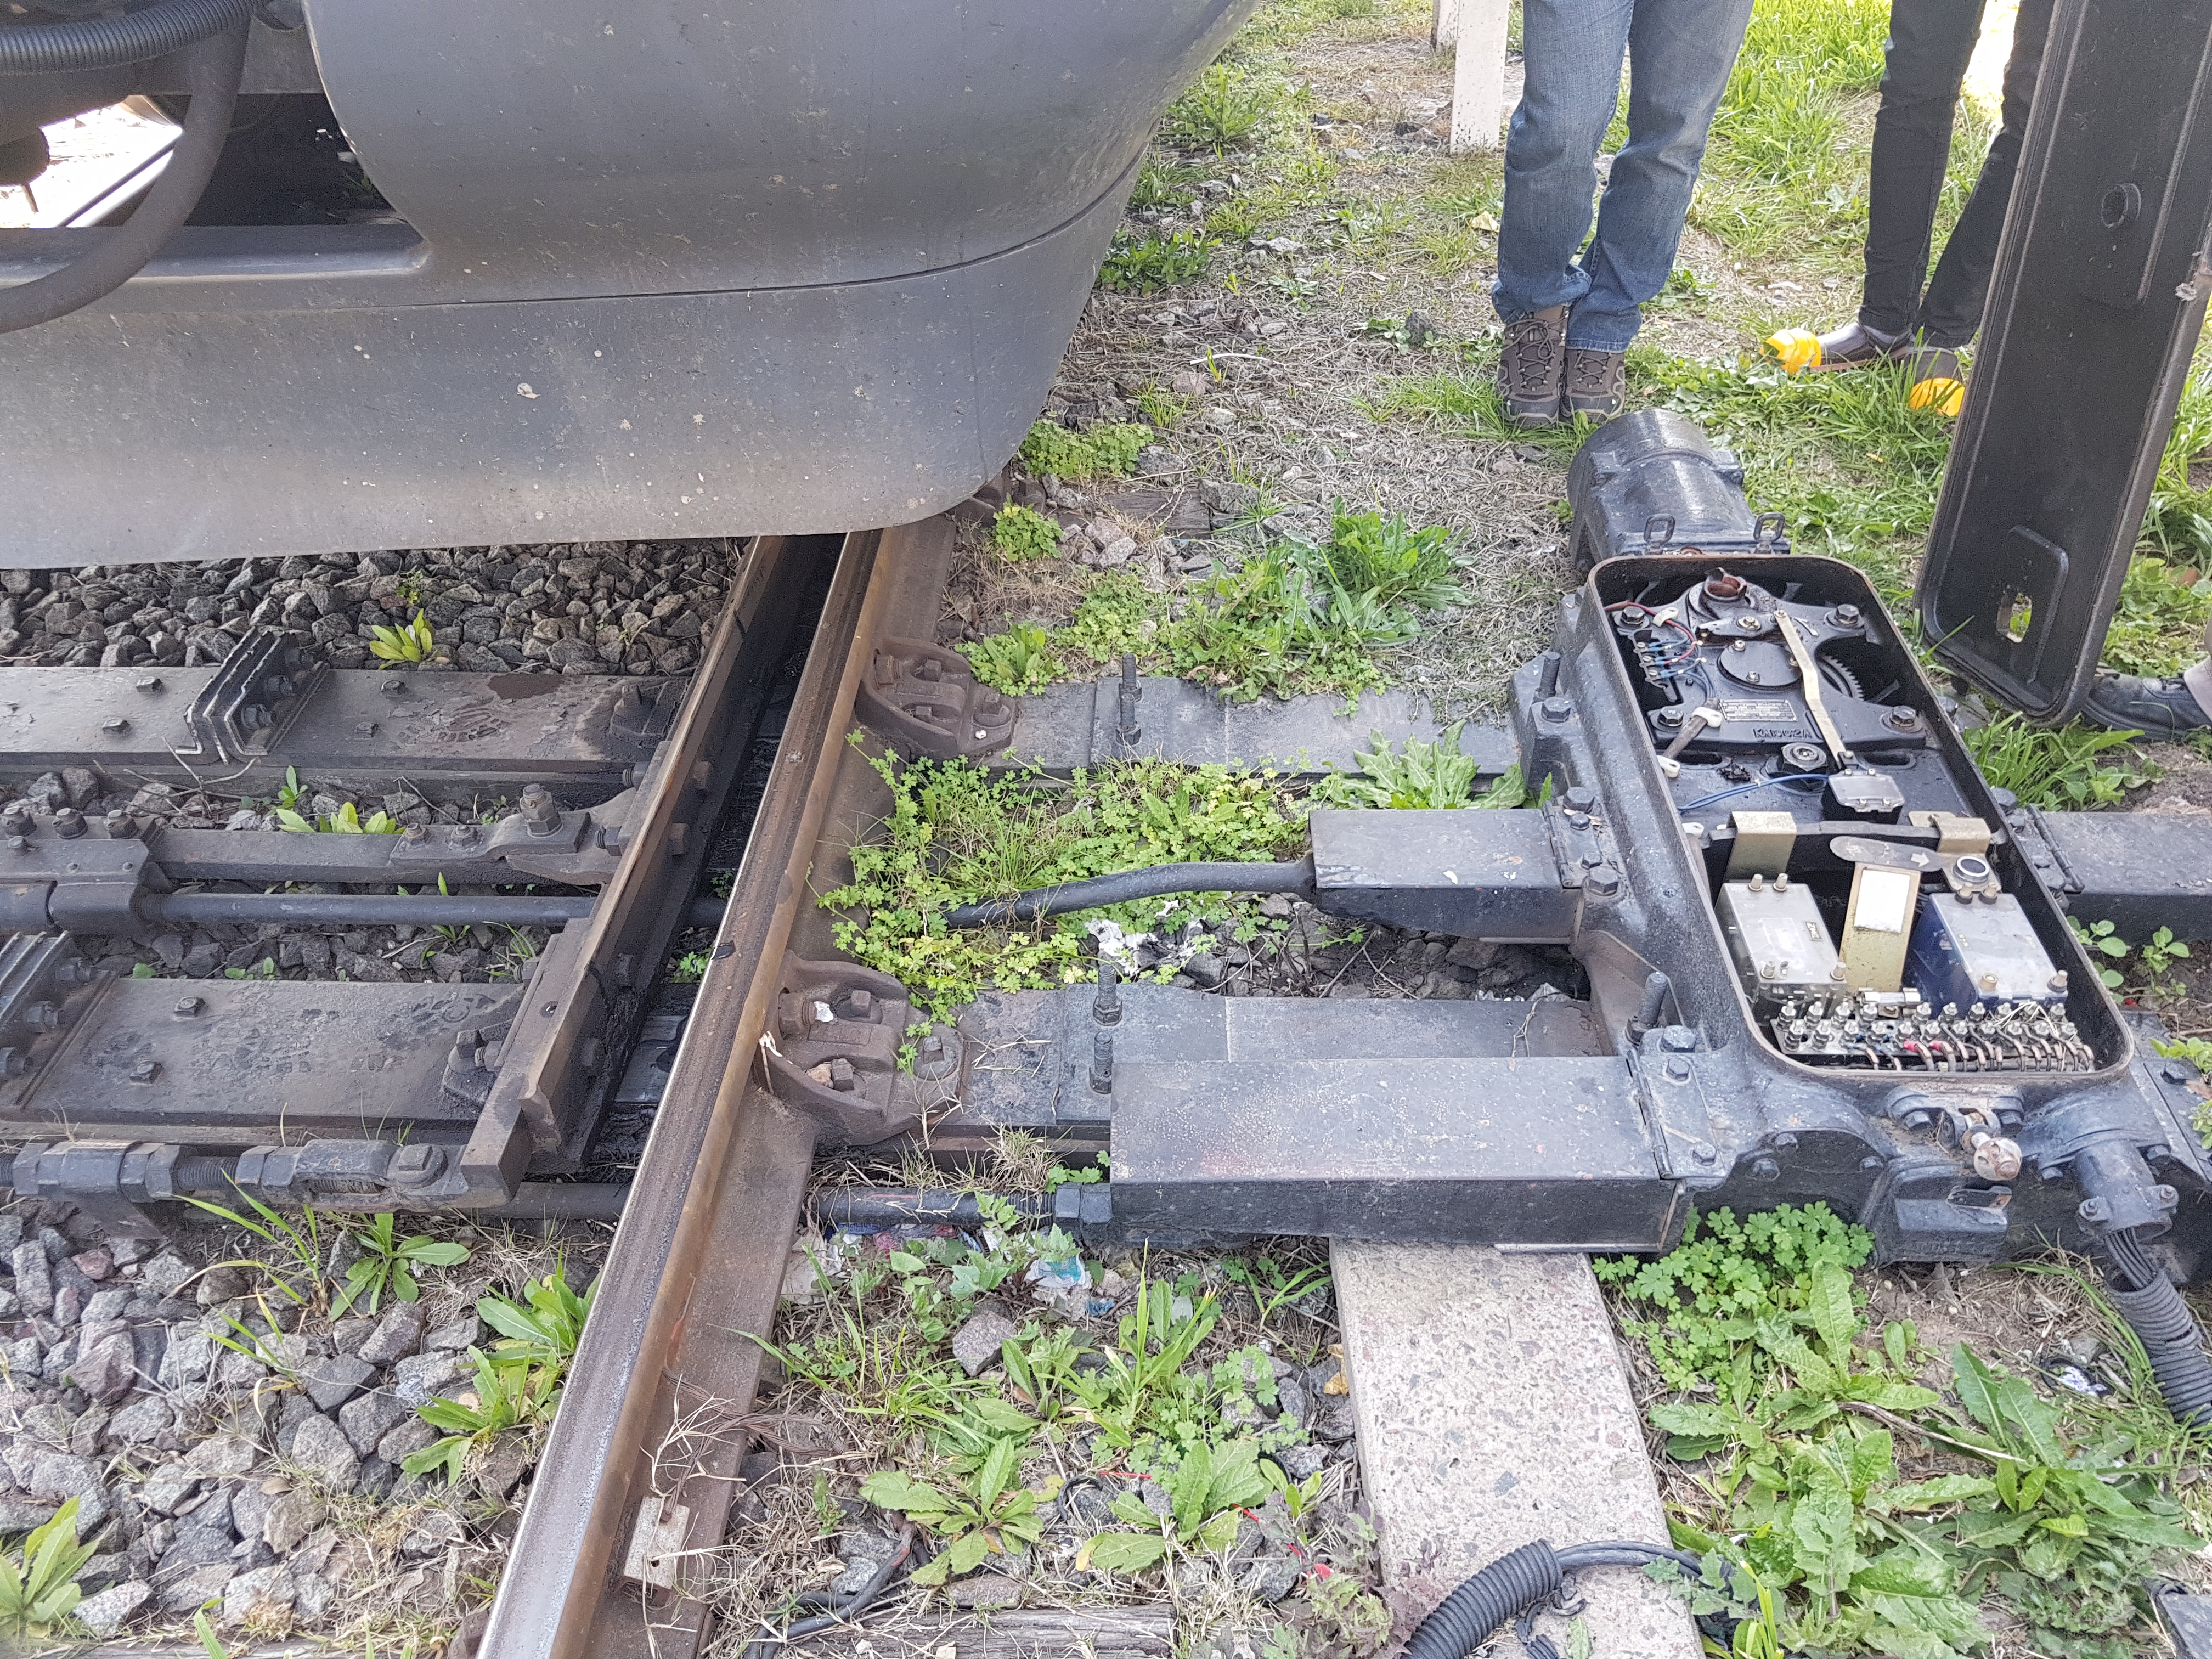
\includegraphics[width=0.75\textwidth]{Figuras/Cambios.jpg}
        \centering\caption{Máquina de cambios.}
        \label{fig:cambios_1}
    \end{figure}

    En la Figura \ref{fig:cambios_2} se muestra el cambio de vía de la estación Matheu de la Línea Mitre. Se observa que según sea la posición de la máquina de cambios, el tren puede continuar en la misma vía o hacer el cambio a la otra vía.

    \begin{figure}[H]
        \centering
        \includegraphics[width=0.75\textwidth]{Figuras/Cambios_2.jpg}
        \centering\caption{Cambio de vías de estación Matheu, Linea Mitre.}
        \label{fig:cambios_2}
    \end{figure}

    %En la Figura \ref{fig:cambios_3} se muestran las posiciones que puede adoptar el cambio. En la posición normal, los trenes pueden circular de forma directa, en paralelo, por la vía principal en sentidos opuestos. En la posición reversa, por el contrario, se permite el intercambio de trenes de una rama principal a otra en sentido opuesto o a una ramificación secundaria de la red.

   % \begin{figure}[H]
   %     \centering
   %     \includegraphics[width=1\textwidth]{Figuras/cambio_3.PNG}
   %     \centering\caption{Posiciones adoptadas por un cambio de vías simple.}
   %     \label{fig:cambios_3}
   % \end{figure}

    Al ser mecanismos que necesitan tiempo para cambiar de un estado al otro, no puede asumirse que el comando es obedecido al instante. Incluso podría darse el caso que jamás llegue a cumplirse la orden debido a desperfectos mecánicos o eléctricos. Es por eso que introducimos los conceptos de comando, indicación y correspondencia, tal como se ilustran en la Figura \ref{fig:cambios_4}.

    \begin{figure}[H]
        \centering
        \includegraphics[width=1\textwidth]{Figuras/cambios}
   \textit{}     \centering\caption{Comando, indicación y correspondencia en un cambio de vías.}
        \label{fig:cambios_4}
    \end{figure}
    
    El comando es la instrucción que el sistema de enclavamientos envía a la máquina de cambios. Esta instrucción puede ser modificar la posición de normal a reverso o de reverso a normal. La indicación es el estado que la máquina de cambios informa al sistema de enclavamientos. El sistema solo asume que el comando fue obedecido cuando tanto el comando como la indicación muestran una correspondencia. En caso contrario, el sistema de enclavamiento no puede asumir cual es el estado real del sistema, si el comando enviado o el estado reportado por la máquina de cambios. El mismo concepto puede ser aplicado en cualquier otro elemento mecánico, como por ejemplo las barreras ferroviarias.

    El RNA debe analizar diversos atributos distribuidos entre la clase \textit{switchIS} (Código \ref{lst:switchIS}), la clase \textit{spotElementProjection} (Código \ref{lst:switch}) y la clase \textit{switchIL} (Código \ref{lst:switchIL}). La clase \textit{switchIS} se encuentra dentro del vector de clases \textit{switchesIS}, dentro de la clase \textit{functionalInfrastructure}, que a su vez es parte de la clase infrastructure. La clase \textit{switchIS} define el id de la máquina de cambios, el tipo (ordinario), el \textit{netElement} al cual pertenece la entrada del cambio y hacia que lado se encuentra la vía de continuación y ramificación si transitamos desde el \textit{netElement} del cambio hacia el cambio mismo. En este caso, si transitamos por el \textit{netElement} ne16 el tren tendrá la vía de continuación en la mano derecha y la ramificación en la mano izquierda. Los cambios de vías simples ("ordinarySwitch") siempre tienen una rama izquierda y una rama derecha definida. Además, dentro de la definición de cada rama tenemos el atributo \textit{netRelationRef}, del cual se puede obtener, procesamiento mediante, los otros \textit{netElement} correspondientes a las ramas: ne15 y ne14.

    \begin{lstlisting}[language = XML, caption = Clase \textit{switchIS} , label = {lst:switchIS}]
    <switchIS id="swi84" continueCourse="right" branchCourse="left" type="ordinarySwitch">
        <name name="Sw01" language="en"/>
        <spotLocation id="swi84_sloc01" netElementRef="ne16" applicationDirection="reverse" intrinsicCoord="0.0000"/>
        <designator register="_Example" entry="SWITCH Sw01"/>
        <leftBranch netRelationRef="nr_ne15ne16_swi84" branchingSpeed="0" joiningSpeed="0" radius="-500"/>
        <rightBranch netRelationRef="nr_ne14ne16_swi84" branchingSpeed="0" joiningSpeed="0" radius="0"/>
    </switchIS>
    \end{lstlisting}

    La clase \textit{spotElementProjection} define la ubicación en el espacio del elemento ferroviario referido. En este caso, como se puede ver en el Código \ref{lst:switch}, la posición de la máquina de cambios es la coordenada (-561 ; -450).

    \begin{lstlisting}[language = XML, caption = Clase \textit{spotElementProjection} , label = {lst:switch}]
    <spotElementProjection refersToElement="swi84" id="vis01_sep16">
        <name name="Sw01" language="en"/>
        <coordinate x="-560.994" y="-450.000"/>
    </spotElementProjection>
    \end{lstlisting}

    La clase \textit{switchIL}, definida dentro del vector de clases \textit{switchesIL}, se encuentra dentro de la clase \textit{assetsForIL}, en la clase \textit{interlocking}. Contiene datos extra sobre el comportamiento dinámico del cambio de vías y define explícitamente los otros dos nodos, en contraposición a \textit{switchIS} del cual hay que obtenerlos procesando un string. El RNA puede obtener los \textit{netElement} de ambas clase y compararlos, anulando el análisis si los \textit{netElement} definidos en \textit{switchIS} y \textit{switchIL} no son coincidentes.
    
    \begin{lstlisting}[language = XML, caption = Clase \textit{SwitchIL} , label = {lst:switchIL}]
    <switchIL id="il_swi84" maxThrowTime="PT10S" typicalThrowTime="PT6S" isKeyLocked="false" returnsToPreferredPosition="false">
        <refersTo ref="swi84"/>
        <branchLeft ref="ne15"/>
        <branchRight ref="ne14"/>
    </switchIL>
    \end{lstlisting}
    
    El RNA utiliza el Algoritmo \ref{alg:switches} para detectar todos estos parámetros y crear un vector de máquinas de cambios (switches) indexado por el id de cada máquina de cambios (sw\_id). La existencia y ubicación de las máquinas de cambios ya se habían obtenido mediante el análisis de la red de grafos ferroviaria. El Algoritmo \ref{alg:switches} analiza la clase \textit{switchIS} y confirma la existencia de la máquina de cambios, para luego la clase \textit{spotElementProjection} y confirmar la ubicación de la misma. Los datos obtenidos en switches[sw\_id].LeftBranch y switches[sw\_id].RightBranch, permiten obtener los nodos de las ramificaciones que luego se conformarán analizando la clase \textit{switchIL} en algoritmos posteriores.

    \begin{algorithm}[H]\captionsetup{labelfont={sc,bf}, labelsep=newline}
            \caption{Algoritmo detector de cambios de vías.}
            \label{alg:switches}
            \begin{algorithmic}
                \STATE \{switches\} $\gets$ \{\}
                \IF {infrastructure.SwitchesIS != None} 
                    \FOR{i in infrastructure.SwitchesIS[0].SwitchIS}
                        \IF{i.Id not in switchesIS.keys()}
                            \STATE sw\_id $\gets$ i.Name[0].Name
                            \STATE j $\gets$ i.SpotLocation[0]
                            \STATE node $\gets$ j.NetElementRef
                            \STATE type $\gets$ i.Type
                            
                           	\IF{type == 'OrdinarySwitch'}
	                           	\STATE left\_id $\gets$ i.LeftBranch[0].NetRelationRef
	                           	\STATE right\_id $\gets$ i.RightBranch[0].NetRelationRef
	                           	\STATE switches[sw\_id] $\gets$ \{"Node":node\}
	                           	\STATE switches[sw\_id] $\gets$ \{"Continue":i.ContinueCourse\}
	                           	\STATE switches[sw\_id] $\gets$ \{"Branch":i.BranchCourse\}
	                           	\STATE switches[sw\_id] $\gets$ \{"Dir":j.ApplicationDirection\}
	                           	\STATE switches[sw\_id] $\gets$ \{"LeftBranch":j.left\_id\}
	                           	\STATE switches[sw\_id] $\gets$ \{"RightBranch":j.right\_id\}
                            \ENDIF
                            \IF{type == 'DoubleSwitchCrossing'}
	                            \STATE straightBranch\_A\_id $\gets$ i.StraightBranch[0].NetRelationRef
	                            \STATE straightBranch\_B\_id $\gets$ i.StraightBranch[1].NetRelationRef
	                            \STATE turningBranch\_A\_id $\gets$ i.TurningBranch[0].NetRelationRef
	                            \STATE turningBranch\_B\_id $\gets$ i.TurningBranch[1].NetRelationRef
	                            
	                            \FOR{X,Z combination(A,B)}
		                            \STATE switches[sw\_id+'XZ'] $\gets$ \{"Node":node\}
		                            \STATE switches[sw\_id+'XZ'] $\gets$ \{"Continue":i.ContinueCourse\}
		                            \STATE switches[sw\_id+'XZ'] $\gets$ \{"Branch":i.BranchCourse\}
		                            \STATE switches[sw\_id+'XZ'] $\gets$ \{"Dir":j.ApplicationDirection\}
		                            \STATE switches[sw\_id+'XZ'] $\gets$ \{"LeftBranch":j.straightBranch\_X\}
		                            \STATE switches[sw\_id+'XZ'] $\gets$ \{"RightBranch":j.turningBranch\_Z\}
	      						\ENDFOR
                            \ENDIF
                            
                        \ENDIF
                    \ENDFOR
                \ENDIF
                \STATE visual\_data $\gets$ visualization.Visualization
                \IF {visual\_data != None}
                    \FOR {i in  visual\_data[0].SpotElementProjection}
                        \STATE sw\_id $\gets$ i.Name[0].Name
                        \IF {'Sw' in sw\_id}
                            \STATE pos\_x $\gets$ int(i.Coordinate[0].X)
                            \STATE pos\_y $\gets$ int(i.Coordinate[0].Y)
                            \STATE switches[sw\_id] $\gets$ \{"Position":[pos\_x,-pos\_y]\}
                        \ENDIF 
                    \ENDFOR
                \ENDIF
            \OUTPUT \{switches\}
            \end{algorithmic}
        \end{algorithm}
    
    % SEMAFOROS
    \subsection{Semaforos}

\lipsum[1]
\section{Redes de grafos}
    \label{sec:grafos}

    \lipsum[1]
\section{Algoritmos de generacion de señalamiento}

\lipsum[1]

\subsection{Fin de via}

\lipsum[1]

\begin{algorithm}[hbt!]
            \caption{Line border and buffer stops algorithm}\label{alg:LBBS}
            \DontPrintSemicolon
            %\SetAlgoLined
            \SetNoFillComment
            \LinesNotNumbered 
            \For { netElement WITH BufferStops }
            {
                \If { NOT EXIST next netElement }
                {
                    [Signals] $\gets$ ADD stop signal $>>$\;
                    [Signals] $\gets$ ADD departure signal $<<$\;
                }
                \If { NOT EXIST prev netElement }
                {
                    [Signals] $\gets$ ADD stop signal $<<$\;
                    [Signals] $\gets$ ADD departure signal $>>$\;
                }
            }
            \For { netElement WITH LineBorder }
            {
                \If { netElement.Length $>$ FIXED\_LENGTH }
                {
                    \If { NOT EXIST next netElement }
                    {
                        [Signals] $\gets$ ADD departure signal $>>$\;
                    }
                    \If { NOT EXIST prev netElement }
                    {
                        [Signals] $\gets$ ADD departure signal $<<$\;
                    }
                }
            }
            \KwResult{[Signals]} 
        \end{algorithm}
\subsection{Detectores}

\lipsum[1-2]

\begin{algorithm}[hbt!]
            \caption{Train detection elements algorithm}\label{alg:RJ}
            \DontPrintSemicolon
            %\SetAlgoLined
            \SetNoFillComment
            \LinesNotNumbered 
            \For { netElement WITH AxleCounters or RailJoints }
            {
                Track.Length = Length ( between RailJoints )\;
                \If { Track.Length $>$ FIXED\_LENGTH }
                {
                    [Signals] $\gets$ ADD circulation signal $>>>$\;
                    [Signals] $\gets$ ADD circulation signal $<<<$\;
                }
            }
            \KwResult{[Signals]} 
        \end{algorithm} 

\lipsum[1]
\includegraphics{example-image}\\
\lipsum[1]
\subsection{Plataformas ferroviarias}

    % Autoridad > derecho limitado a una porcion
    % Claridad > autoridad no ambigua
    % Anticipacion > avisar con antelacion
    % Granularidad > rutas cortas y funcionales
    % Terminalidad > avisar fin de via
    % Infraestructura > avisar de infraestructura
    % No bloqueo > circulacion fluida

    En la Sección \ref{sec:platform} definimos la clase platform que modela a las plataformas ferroviarias. Las plataformas ferroviarias son un punto del recorrido donde las formaciones pueden detenerse, algunas veces de forma opcional dependiendo el itinerario, para que los pasajeros desciendan y nuevos pasajeros puedan ascender. Claramente existe una limitación de autoridad, las formaciones necesitan un nuevo permiso para continuar circulando una vez alcanzada la plataforma. Permiso que será otorgado o negado según el estado del sistema a continuación del recorrido. Las plataformas ferroviarias suelen encontrarse en zonas pobladas, cerca de otras infraestructuras, zonas comerciales o residenciales, por lo que avisar con antelación al maquinista que debe disminuir la marcha y/o detenerse es esencial.

    Además, es posible que las formaciones convivan con otras formaciones que también hacen uso de la estación, por lo que las señales deben ser unívocas y claras. Algunas estaciones pueden contener fines de vías o ramificaciones hacia talleres u otros ramales, por lo que también se aplica el principio de terminalidad y granuralidad. Finalmente, es importante el mantener una circulación fluida de las formaciones, de modo de no retrasar el itinerario de las formaciones que vienen detrás, por lo que se deberá aplicar el principio de no bloqueo.

    En el Algoritmo \ref{alg:PTF} definimos a la señal de partida como la única señal necesaria para operar una plataforma, asumiendo que la señal de ingreso de la misma será dada por otra instancia previa. De no existir otro elemento cercano por el cual se genere una señal, se puede asumir que la distancia a la plataforma es muy larga y, por lo tanto, se aplicaría el Algoritmo \ref{alg:RJ}, protegiendo a la plataforma. En el caso de que la vía se bidireccional se añadiran señales de partida para ambos sentidos.

    \begin{algorithm}[hbt!]
        \caption{Algoritmo de generación de señalamiento para platforms.}\label{alg:PTF}
        \DontPrintSemicolon
        %\SetAlgoLined
        \SetNoFillComment
        \LinesNotNumbered 
        \For { netElement WITH Platform }
        {
            \tcc{Before leaving platform from left}
            [Signals] $\gets$ ADD departure signal $\gg\gg$\;
            \tcc{After leaving platform from right}
            [Signals] $\gets$ ADD departure signal $\ll\ll$\;
        }
        \KwResult{[Signals]} 
    \end{algorithm}

    Aplicando el Algoritmo \ref{alg:PTF} a un sistema de dos vías paralelas con plataformas pertenecientes a la misma estación obtenemos el resultado ilustrado en la Figura \ref{fig:signal_platform}.Se asumieron que ambas vías son bidireccionales, en caso contrario solo se generarían las señales S01 y S02.
    
    \begin{figure}[h!]
        \centering
        \includegraphics[width=1\textwidth]{Figuras/platforms.PNG}
        \centering\caption{Señalamiento generado para estaciones ferroviarias.}
        \label{fig:signal_platform}
    \end{figure}
    
    Una formación que circule de izquierda a derecha deberá detenerse antes de la señal S01, en caso de utilizar la vía superior, o antes de la señal S04, en caso de utilizar la vía inferior. Análogamente, las formaciones deberán detenerse antes de las señales S03 y S02 en el caso de transitar de derecha a izquierda por la vía superior o inferior respectivamente. Sólo cuando estas señales otorguen a la formación autoridad para circular podrán reanudar su marcha hasta la próxima señal disponible, fuera del alcance de lo ilustrado en la Figura \ref{fig:signal_platform}.
\subsection{Cruces de via}

\lipsum[1]

\begin{algorithm}[hbt!]
            \caption{Level crossing algorithm}\label{alg:LC}
            \DontPrintSemicolon
            %\SetAlgoLined
            \SetNoFillComment
            \LinesNotNumbered 
            \For { netElement WITH LevelCrossing }
            {
                \tcc{Before reaching level crossing}
                [Signals] $\gets$ ADD circulation signal $>>>$\;
                \tcc{After leaving level crossing}
                [Signals] $\gets$ ADD circulation signal $<<<$\;
            }
            \KwResult{[Signals]} 
        \end{algorithm}
\subsection{Maquinas de cambios}

    \lipsum[1-2]

    \begin{algorithm}[hbt!]
        \caption{Switch algorithm}\label{alg:SW}
        \DontPrintSemicolon
        %\SetAlgoLined
        \SetNoFillComment
        \LinesNotNumbered 
        \For { Switch in Switches }
        {
            \tcc{All signals must point to switch}
            \Switch{ Switch.Type }
            {
                \Case{Start}
                {
                    [Signals] $\gets$ ADD circulation signal\;
                    [Signals] $\gets$ ADD maneuver signal\;
                }
                \Case{Continue branch}
                {
                    [Signals] $\gets$ ADD circulation signal\;
                }
                \Case{Detour branch}
                {
                    [Signals] $\gets$ ADD maneuver signal\;
                }
            }   
        }
        \KwResult{[Signals]} 
    \end{algorithm}

    \lipsum[1]
    \includegraphics{example-image}\\
    \lipsum[1-2]
\section{Algoritmos de simplificacion de señalamiento}

\lipsum[1]

\subsection{Algoritmo de herencia horizontal}

    \lipsum[1-3]

    \begin{algorithm}[hbt!]
        \caption{Horizontal inheritance algorithm}\label{alg:horizontal}
        \DontPrintSemicolon
        %\SetAlgoLined
        \SetNoFillComment
        \LinesNotNumbered 
        \For{ each netElement }
        {
            \For{ each object in netElement }
            {
                \If{dist(Obj\_A,Obj\_B) $<$ MIN\_DISTANCE }
                {
                    move\_signals\_between(Obj\_A,Obj\_B)
                }
            }
        }
        \KwResult{[Signals]} 
    \end{algorithm}

    \lipsum[1-3]
\subsection{Algoritmo de simplificación por herencia vertical}
	\label{sec:vertical}
	% Autoridad > derecho limitado a una porcion
	% Claridad > autoridad no ambigua
	% Anticipacion > avisar con antelacion
	% Granularidad > rutas cortas y funcionales
	% Terminalidad > avisar fin de via
	% Infraestructura > avisar de infraestructura
	% No bloqueo > circulacion fluida
	
	Como se explicó en la Sección \ref{sec:switches}, una máquina de cambios bifurca la vía principal en dos: una vía que continúa la rama principal y otra vía que se convierte en una rama secundaria. Tanto la vía de continuación como la vía ramificada pueden tener otra máquina de cambios que, a su vez, vuelve a dividir el trazado ferroviario en dos. Esto incrementa más y más el nivel de complejidad de la red, añadiendo caminos divergentes al principal que luego, mas adelante, podrían, o no, volver a converger utilizando mas máquinas de cambios. Cada divergencia aporta un nivel de profundidad a la red, mientras que cada convergencia reduce en uno el nivel de profundidad.
	
	Una máquina de cambios que tiene en cualquiera de sus ramas divergentes el nodo de inicio de otra máquina de cambios a una distancia pequeña es un cambio compuesto. Los cambios compuestos requieren considerar a ambas máquinas de cambios como una sola, ya que es necesario posicionar ambos mecanismos para completar un movimiento. El ejemplo de La Figura \ref{fig:signal_vertical_1} ayudará a clarificar el concepto de cambios compuestos e introducir el Algoritmo de simplificación por herencia vertical.	

	\begin{figure}[h!]
		\centering
		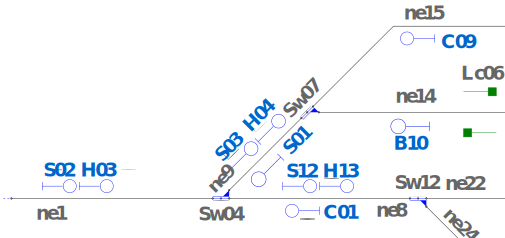
\includegraphics[width=1\textwidth]{Figuras/Figure8_Crop.pdf}
		\centering\caption{Señalamiento generado, simplificado por algoritmo de herencia vertical.}
		\label{fig:signal_vertical_1}
	\end{figure}
	
	En la Sección \ref{sec:signal_switches} se introdujo el Algoritmo \ref{alg:SW} que define la asignación de señalamiento para los cambios de vías: una señal de circulación (S) y de maniobra (H) para el nodo de inicio (S), una señal de circulación para el nodo de continuación (C) y una señal de maniobras para el nodo de desvío (B). El Algoritmo \ref{alg:SW} se aplicó de forma independiente a las máquinas de cambios Sw04, Sw07 y Sw12 y se obtuvo el señalamiento de la Figura \ref{fig:signal_vertical_1}. No obstante, el señalamiento generado no cumple con el principio de no bloqueo, al situar las señales S03, H04, B01, S12, H13 y C01 en las secciones correspondientes a los netElements ne9 y ne8. De esa manera, las formaciones podrían detenerse en esas secciones si las mencionadas señales presentasen un aspecto rojo.
	
	Una formación detenida en la sección correspondiente al netElement ne9 no permitiría mover el cambio de vía Sw04, al tener parte de la formación aún en ne1. Tampoco permitiría accionar el cambio de vías Sw07 al no haber finalizado el movimiento. Análogamente para una formación detenida en la sección correspondiente al netElement ne8. Es necesario que el movimiento finalice, despejando las secciones y permitiendo que otras formaciones utilicen los cambios de vías Sw04 y Sw07, o cualquier combinación de mas de un cambio de vías.
	
	Para solucionar el problema expuesto, el RNA aplica el Algoritmo \ref{alg:vertical} de simplificación por herencia vertical para reposicionar las señales situadas en zonas conflictivas. A diferencia del señalamiento explicado en la Sección \ref{sec:generacion}, las señales que protegen a un cambio de vías B situado en una rama mas profunda de la red no se encuentran inmediatamente precediendo al cambio de vías B. Estas señales son movidas a ramas de menor profundidad con suficiente espacio físico para contenerlas, situándose precediendo a otro cambio de vías A que decimos que ha \emph{heredado} el señalamiento del cambio de vía B.
		
	\begin{algorithm}[hbt!]
        \caption{Algoritmo de simplificación por herencia vertical}\label{alg:vertical}
        \DontPrintSemicolon
        %\SetAlgoLined
        \SetNoFillComment
        \LinesNotNumbered 
        \For{ each Signal protecting a Sw\_A }
        {
            \For{each Sw\_B != Sw\_A}
            {
                \tcc{Criteria \#0}
                \If{distance(Sw\_A,Sw\_B) $>$ MIN\_DISTANCE}
                {
                    Continue\;
                }
                \If{S in Sw\_A.Branch also in Sw\_B.Start} 
                {
                   \tcc{Criteria \#1}
                   \If{S points to Sw\_B.Start}
                   {
                        Move S to Sw\_A.Start\;
                   }
                   \tcc{Criteria \#2}
                   \If{S points to Sw\_A.Branch}
                   {
                        Move S to Sw\_B.Continue\;
                        Move S to Sw\_B.Branch\;
                   }
                }
                \If{S in Sw\_A.Continue also in Sw\_B.Start}
                {
                   \tcc{Criteria \#3}
                   \If{S points to Sw\_B.Start}
                   {
                        Move S to Sw\_A.Start\;
                   }
                   \tcc{Criteria \#4}
                   \If{S points to Sw\_A.Continue}
                   {
                        Move S to Sw\_B.Continue\;
                        Move S to Sw\_B.Branch\;
                   }
                }
            }
        
        }
        \KwResult{[Signals]} 
    \end{algorithm}

    Como puede apreciarse en el Algoritmo \ref{alg:vertical}, existen cinco criterios a considerar para aplicar la herencia vertical. El primer criterio es excluyente, si la distancia entre ambas máquinas de cambios supera un parámetro determinado entonces el algoritmo no se aplica, al existir suficiente distancia para situar el señalamiento sin generar obstrucciones debido a formaciones detenidas entre ambos. Cuando la distancia entre las máquinas de cambios es menor a lo esperado, se aplican los otros cuatro criterios, en función de que nodos conectan entre sí la vía que comparten.
    
    Definiendo al cambio de vías A como el cambio principal y el cambio de vías B como el cambio secundario situado en alguna de las ramificaciones del cambio de vías A, podemos diferenciar dos casos: que el señalamiento se encuentre en la rama de continuación del cambio de vías A o se encuentre en la rama de desvío. A su vez, este señalamiento puede estar apuntando al cambio de vías A o al cambio de vías B, protegiéndolo respectivamente. 
    
    El criterio para el desplazamiento del señalamiento busca cumplir el principio de Anticipación, el principio de Infraestructura y el principio de no bloqueo. Para eso, las señales son adelantadas, desplazándolas en sentido opuesto al que apuntan. Si el señalamiento se encuentra en la rama de desvío o continuación del cambio de vías A es indistinto, lo importante es a donde apuntan las señales. Si estas apuntan hacia el nodo de inicio del cambio de vías B, deben ser desplazadas, sin alterar su cantidad, hacia el nodo de inicio del cambio de vías A. 
    
    En el caso particular de que las señales en la zona conflictiva apunten hacia el cambio de vías A, tanto a su nodo de desvío como al nodo de continuidad, las mismas deberían moverse en sentido contrario al que apuntan. Pero en esa dirección la red se ramifica en dos debido al cambio de vías B. En este caso, las señales mueven duplicadas, a la rama de continuación y a la rama de desvío del cambio de vías B, en su totalidad.
    
    Aplicando el Algoritmo \ref{alg:vertical} de herencia vertical al ejemplo de la Figura \ref{fig:signal_vertical_1} obtenemos el señalamiento de la Figura \ref{fig:signal_vertical_2}. Las señales S03, H04, B01, S12, S13 y C01 serán adelantadas para despejar las secciones correspondientes a los netElements ne9 y ne8. Debido a esto, los tres cambios de vías se usarán de forma complementaria, creando los siguientes cambios compuestos: $Sw_{04}^R+Sw_{07}^N$, $Sw_{04}^R+Sw_{07}^R$, $Sw_{04}^N+Sw_{12}^N$ y $Sw_{04}^N+Sw_{12}^R$. Los cuales se leen, considerando el ejemplo del cambio compuesto $Sw_{04}^R+Sw_{07}^N$, de la siguiente manera: el cambio de vías Sw04 en posición normal y el cambio de vías Sw07 en posición reversa.
    
    \begin{figure}[h!]
    	\centering
    	\includegraphics[width=1\textwidth]{Figuras/Figure9_Crop.pdf}
    	\centering\caption{Señalamiento generado, simplificado por algoritmo de herencia vertical.}
    	\label{fig:signal_vertical_2}
    \end{figure}
    
    En el caso de las señales S03 y H04 que apuntan al nodo de inicio del cambio de vías Sw07, son desplazadas en sentido contrario al que apuntan, aplicando el criterio \#1. Estas señales son movidas hasta el nodo de continuación del cambio de vías Sw04, correspondiente al netElement ne1, protegiendo el inicio del cambio compuesto $Sw_{04}^R+Sw_{07}^N$ y $Sw_{04}^R+Sw_{07}^R$ . A estas señales se le suman las señales S12 y H13 situadas en la sección correspondiente al netElement ne8 que, aplicando el criterio \#3, son desplazadas al nodo de inicio del cambio de vías Sw04, protegiendo el inicio del cambio compuesto $Sw_{04}^N+Sw_{12}^N$ y $Sw_{04}^N+Sw_{12}^R$.
    
    La señal B01 apunta al nodo de desvío del cambio de vías Sw04 y, por el criterio \#2, debe ser duplicada y movida. Una señal se posiciona en la sección correspondiente al netElement ne15 y la otra a la sección asociada al netElement ne14. De esta manera, la señal S01a y S01b seguirán protegiendo el nodo de desvío del cambio de vías Sw04, pero previamente tendrán que hacer uso del cambio de vías Sw07 en cualquiera de sus dos posiciones, protegiendo los nodos de cambio y continuación del cambio compuesto $Sw_{04}^R+Sw_{07}^N$ y $Sw_{04}^R+Sw_{07}^R$. De igual manera, la señal C01 es movida y duplicada a las secciones correspondientes a los netElements ne22 y ne24, debido al criterio \#4. Estas nuevas señales C01a y C01b continúan protegiendo el nodo de continuación del cambio de vías Sw04, pero ahora deberán, adicionalmente, hacer uso del cambio de vías Sw12, protegiendo los nodos de continuación y desvío del cambio compuesto $Sw_{04}^N+Sw_{12}^N$ y $Sw_{04}^N+Sw_{12}^R$.
    
    El Algoritmo \ref{alg:vertical} de herencia vertical es exitoso a la hora de despejar las zonas críticas entre cambios de vías muy cercanos. No obstante, también incrementa la cantidad de señales, como en el caso de las señales S01 y C01 al ser desplazadas en sentido divergente por los cambios de vías Sw07 y Sw12. Además, el Algoritmo \ref{alg:vertical} de herencia vertical no es aplicable solo a una dupla de cambios de vías, sino que puede ser aplicado para cualquier conjunto de cambios de vías. Esto provoca que las señales se hereden de forma iterativa hasta encontrar un cambio de vías con suficiente espacio para albergar las señales. Debido a esto, la cantidad de señales al comienzo de un cambio de vías previo a una ramificación profunda de la red tendrá una gran cantidad de señales.
    
    En el caso del ejemplo de las Figuras \ref{fig:signal_vertical_1} y \ref{fig:signal_vertical_2}, el algoritmo concluye con seis señales en el nodo de inicio de los cuatro cambios compuestos. Estas seis señales deberán habilitar cuatro caminos a transitar desde ne1: hacia ne15, hacia ne14, hacia ne22 y hacia ne24. Es claro que, teniendo mas señales que caminos a habilitar, será necesario un algoritmo de limpieza de señales duplicadas y/o que ya no tengan una utilidad en el señalamiento. El proceso de simplificación es explicado en profundidad en la Sección \ref{sec:limpieza}.
\subsection{Limpieza de señales}

Prioridad y repetición
\lipsum[1]

\begin{algorithm}[hbt!]
        \caption{Signal reduction algorithm}\label{alg:reduction}
        \DontPrintSemicolon
        %\SetAlgoLined
        \SetNoFillComment
        \LinesNotNumbered 
        Sources = $\{$ T,L,S,B,P,C,J,X $\}$\;
        \For{ Sig\_A \& Sig\_B in [Signals]}
        {
            \If{ A != B  \& Sig\_A.From == Sig\_B.From }
            {
             CDL\_zones.Pos = detect\_next\_dangers ( Sig\_A )\;
             A.Pos,B.Pos = Sig\_A.Pos,Sig\_B\;
             Safe = zone\_between(CDL\_zones.Pos,A.Pos,B.Pos)\;
                 \If{ NOT safe }
                 {
                    \If{ $|A.Pos,B.Pos|$ $<$ MIN\_DISTANCE }
                    {
                        \If{ Sig\_A \& Sig\_B same orientation }
                        {
                            \If{ Sig\_A \& Sig\_B same direction }
                            {
                                \If { Sig\_A \& Sig\_B type "Circ" }
                                {
                                    \If{ Sig\_A.Idx $<$ Sig\_B.Idx }
                                    {
                                        delete Sig\_B  else Sig\_A
                                    }
                                    %{
                                    %    delete( Sig\_A )
                                    %}
                                }
                            }
                        }
                        \If{ Sig\_A \& Sig\_B different source}
                        {
                            delete\_lowest\_priority( Sig\_A,Sig\_B )\;
                        }
                    }
                }
            }
        }
        \KwResult{[Signals]} 
    \end{algorithm}

    \lipsum[1-3]

\section{Generación de tablas de enclavamiento}

	\label{sec:rutas}
	
	% Once the signalling is generated and simplified, it is necessary to establish the railway routes to create the railway interlocking table. A railway route is the simplest path between two consecutive signals in the same direction, using the same tracks \cite{SIGNALLING_1,AUTOMATIC_SIMPLE_SIGNAL}. The route may contain switches, level crossings, platforms or any railway element within the path. A railway route is defined with a start and an end signal, accompanied by the indication of the corresponding safe state of the railway netElements like switches or level crossings and the tracks assigned (P1, P2, P3, P4, P5, P6, P7). Algorithm \ref{alg:routes} describes the mechanisms to detect and assign routes.
	
	\lipsum[1-5]
	
	\begin{algorithm}[hbt!]
        \caption{Route detection algorithm}\label{alg:routes}
        \DontPrintSemicolon
        %\SetAlgoLined
        \SetNoFillComment
        \LinesNotNumbered 
        Routes = []\; 
        route = 0\;
        \For{ start in [Signals] }
        {
            \tcc{Find manoeuvre and circulation signals}
            \If{ start != "Stop" }
            {
                dir = start\_sig.Direction\;
                \tcc{Find next signal w/ same direction}
                
                end = find\_next\_signal(start,[Signals])\;

                [paths] = find(start.node,end.node,graph)\;
                
                \For{ node in [paths] }
                {
                    \tcc{Find rail objects within path}
                    sws = find(graph[node],switches)\;
                    lc = find(graph[node],levelCrossings)\;
                    ptf = find(graph[node],platforms)\;
                    %route ++\;
                    Routes[route++] = $\{$start,end,dir,node,sws,lc,ptf$\}$\;
                }
            }
        }
        \KwResult{[Routes]} 
    \end{algorithm}
    
    %Stop signals cannot be starting signals and, therefore, are ignored, considering only circulation and manoeuvre signals. It is necessary to follow the graph network in the same direction as the starting signal to identify all the incoming signals through all the possible paths from the netElement where the starting signal is. For example, three routes were highlighted in Figure \ref{fig:Routes} over the simplified signalling for Example 1, with signal S22 as the starting signal: S22 to S32, S22 to X15 and S22 to T05.
    
    \lipsum[1-2]
    
    \begin{figure}[h]
    	\centering
    	\includegraphics[width=1\textwidth]{Figuras/Figure11.pdf}
    	\centering\caption{Signalling simplified in Example 1 with three routes indicated.}
    	\label{fig:Routes}
    \end{figure}
    
    %Having the start signal and all the end signals, it is necessary to identify the main rail objects within those paths, such as switches (their position), level crossings (that must be closed), platforms and tracks. In Example 1 (Figure \ref{fig:Routes}), a route defined by signals S22 and T05 covers tracks ne1, ne9 and ne15 using switch Sw04 in reverse position and switch Sw07 in normal position without any level crossing is involved.
    
    %If two routes share the same start signal or end signal they are conflicting routes. The same if they share one netElement, switch, level crossing or the same signals swapped. It means both routes cannot be approved at the same time, one of them being approved implies the others must be blocked until the first one was completed or cancelled. Two routes could have the same start and end signal but use different tracks, but they cannot be approved at the same time because there must be necessary a switch within that routes, with opposite positions and only one position can be approved when one route is ongoing. Conflicting routes are indicated in the interlocking table that is automatically generated by the RNA. Every route is created based on the created graph network and the shortest path algorithm for directed graphs. The paper \cite{GRAPH_4_ROUTES} explores another approach to finding routes based on interlocking tables.
    
    \lipsum[1-3]
\section{Validación de tablas de enclavamiento}

	\lipsum[1-5]
	
	
	\begin{algorithm}[hbt!]
		\caption{Algoritmo de validación de tablas de enclavamiento ferroviarias.}\label{alg:interlocking_tables}
		\DontPrintSemicolon
		%\SetAlgoLined
		\SetNoFillComment
		\LinesNotNumbered 
		old\_graph = create\_Digraph()\; 
		new\_graph = create\_Digraph()\; 
		\tcc{Create digraphs for both interlocking tables}
		\For{start\_net,end\_net,old\_route in old\_table}
		{
			old\_graph $\Leftarrow$ start\_net,end\_net,old\_route\;
		}
		\For{start\_net,end\_net,new\_route in new\_table}
		{
			new\_graph $\Leftarrow$ start\_net,end\_net,new\_route\;
		}
		
		\tcc{Detect coincidences between both digraphs}
		routes\_found = 0\;
		\For{start\_net,end\_net,old\_route in old\_table}
		{
			\If{start\_net != end\_net}
			{
				routes\_found += find\_shortest\_paths(start\_net , end\_net)\;
			}
			\Else
			{
				\If{start\_net in new\_graph}
				{
					routes\_found += 1\;
				}
				\Else
				{
					\If{end\_net in new\_graph}
					{
						begin\_nodes = List(neighbours of end\_net in new\_graph)\;
						
						\If{begin\_nodes != []}
						{
							routes\_found += find\_shortest\_paths(begin\_nodes[0] , end\_net)\;
						}
					}
				}
			}
		
		}

		\KwResult{routes\_found} 
	\end{algorithm}
	
	\lipsum[1-5]
\section{Comprobación de principios de señalamiento ferroviario}
	\label{sec:validar_principios}
	
	% Autoridad > todas las rutas combinadas cubren toda la traza ferroviaria.
	% Claridad > autoridad no ambigua.
	% Anticipacion > avisar con antelacion.
	% Granularidad > rutas cortas y funcionales.
	% Terminalidad > avisar fin de via.
	% Infraestructura > avisar de infraestructura.
	% No bloqueo > circulacion fluida.
				
	En esta sección se abordará el proceso de validación de cada uno de los principios ferroviarios establecidos en la Sección \ref{sec:principios}, como parte del proceso expuesto en la Sección \ref{sec:validacion}. Para ello, serán abordados de manera genérica cada uno de los principios de señalamiento junto con el algoritmo que el RNA utiliza para validarlo, previo a exportar el señalamiento generado.
	
	\subsection{Comprobación del principio de autoridad}
		% Autoridad > todas las rutas combinadas cubren toda la traza ferroviaria.
		
		El principio de autoridad radica en que las rutas otorgan a las formaciones un permiso de uso limitado para circular por las vías. No obstante, la combinación de todas las autoridades disponibles de ser otorgadas deben cubrir la totalidad de la traza ferroviaria. Es decir, no debe existir ninguna sección de vía que se encuentre fuera del alcance de las rutas y, por lo tanto, aislada de la red. Puede darse el caso de que una sección de vía tenga una ruta de entrada o de salida, pero no ambas. También puede darse el caso de que la sección de vía sea transitada, pero no sea ni inicio ni final de ninguna ruta.
		
		El RNA utiliza el Algoritmo \ref{alg:ppio_autoridad} para validar el principio de autoridad comparando los netElements alcanzados por las rutas disponibles, con la lista de netElements potenciales de ser alcanzados. Esta última salvedad deja fuera las secciones de vías que preceden a una señal de circulación posterior a un final de vía relativo (lineBuffer). Esto se realiza ya que estas secciones de vía son transitadas por rutas fuera de la locación bajo análisis, rutas que terminan en la señal de circulación mencionada.

		\begin{algorithm}[H]
			\caption{Algoritmo de validación del principio de autoridad.}\label{alg:ppio_autoridad}
			\DontPrintSemicolon
			%\SetAlgoLined
			\SetNoFillComment
			\LinesNotNumbered 
			Validated = False\;
			$\{$Routes$\}$, $\{$netElements$\}$ without netElements with lineBuffer\; 
			\tcc{Validate that every route covers all the railway tracks.}
			\For{route in $\{$Routes$\}$}
			{
				\If{route[begin] in $\{$netElements$\}$}
				{
					Remove route[begin] from $\{$netElements$\}$\; 
				}
				\If{route[end] in $\{$netElements$\}$}
				{
					Remove route[end] from $\{$netElements$\}$\; 
				}
				\For{track in route[paths]}
				{
					\If{track in $\{$netElements$\}$}
					{
						Remove track from $\{$netElements$\}$\; 
					} 
				}
			}
			\If{$\{$netElements$\}$ is Empty}
			{
				Validated = True\; 
			} 
			\KwResult{Validated} 
		\end{algorithm}
		
		Se asume inicialmente que la validación es fallida por defecto. Si al finalizar el Algoritmo \ref{alg:ppio_autoridad} no existe ningún netElement remanente en la lista, se considera que la validación es exitosa.	
			
	\subsection{Comprobación del principio de claridad}
		% Claridad > autoridad no ambigua
		
		El principio de claridad radica en que el señalamiento no posee señales ambiguas. Es decir, no existen dos rutas distintas que otorguen autoridad sobre las mismas secciones de vía, en el mismo sentido, utilizando la misma infraestructura. En otras palabras, las rutas en una misma dirección y sentido no se solapan, cada una comienza donde otra ha terminado.
		
		El RNA utiliza el Algoritmo \ref{alg:ppio_claridad} para validar el principio de claridad, generando una red de grafos dirigidos. La misma se constituye utilizando todas las rutas definidas por el RNA como aristas, y a los netElements que conectan como nodos de la red. Si se detecta que existen dos rutas R$^{\prime}$ y R$^{\prime\prime}$ que conectan dos nodos A y B en el mismo sentido, utilizando la misma infraestructura, entonces se dice que las rutas son ambiguas y el principio de claridad no se cumple.
		
		\begin{algorithm}[H]
			\caption{Algoritmo de validación del principio de claridad.}\label{alg:ppio_claridad}
			\DontPrintSemicolon
			%\SetAlgoLined
			\SetNoFillComment
			\LinesNotNumbered 
			Validated = False\;
			$\{$Routes$\}$\; 
			\tcc{Validate that every netElement is reached by one route only.}
			\For{route in $\{$Routes$\}$}
			{
				begin = route[begin]\;
				end = route[end]\;
				index = route[index] \;
				direction = route[direction]\;
				digraph = create\_digraph(begin,end,index,direction)\;	
			}
			\If{digraph has no redundant routes}
			{
				Validated = True\;
			}
			\KwResult{Validated} 
		\end{algorithm}
		
		Aunque el orden de validación de los principios de señalamiento es indistinto, la confirmación de que las señales son suficientes para alcanzar toda la red (Principio de autoridad) y de que no existen señales ambiguas (Principio de claridad) facilita las siguientes validaciones. Esto se debe a que, con estas dos comprobaciones, ya sabemos que contamos con la mínima cantidad de señales para recorrer la red de forma unívoca, garantizando la correcta logística de la red. Los siguientes principios son necesarios para validar la seguridad del señalamiento generado por el RNA.
		
	\subsection{Comprobación del principio de anticipación}
		% Anticipacion > avisar con antelacion
		
		El principio de anticipación radica en que existe una señal previo a cada peligro, situada en la zona de señalamiento. Una zona señalamiento puede estar próxima a una curva, al final de la traza ferroviaria o en las inmediaciones de un paso a nivel, una estación, un cambio de vías o cualquier infraestructura ferroviaria a ser protegida. En otras palabras, el señalamiento debe estar distribuido de tal manera que entre dos señales que constituyen una ruta exista un único peligro o situación que quiera la atención del conductor.
		
		El RNA utiliza el Algoritmo \ref{alg:ppio_anticipacion} para validar el principio de anticipación, detectando las regiones de señalamiento como zonas peligro peligrosas, producto del trazado ferroviario (curvas, finales de vía) o de la infraestructura ferroviaria (plataformas, pasos a nivel, etc.). 
		
		\begin{algorithm}[H]
			\caption{Algoritmo de validación del principio de anticipación.}\label{alg:ppio_anticipacion}
			\DontPrintSemicolon
			%\SetAlgoLined
			\SetNoFillComment
			\LinesNotNumbered 
			Validated = True, $\{$Dangers$\}$ = None\;
			$\{$Routes$\}$, $\{$Track$\}$\; 
		
			\tcc{Validate that each danger is protected by the signalling.}
			
			\For{curve in $\{$Tracks$\}$}
			{
				$\{$Dangers$\}$ $\Leftarrow$ ADD curve
			}
			
			\For{element in $\{$Infraestructure$\}$}
			{
				$\{$Dangers$\}$ $\Leftarrow$ ADD element
			}
			
			\For{danger in $\{$Dangers$\}$}
			{
				
				\For{track going into danger}
				{
					\If{track has signal AND signal points to danger}
					{
						Continue\;
					}
					\Else
					{
						Validated = False\; 
						Stop iterations\;
					}
				}	
			}
			
			\KwResult{Validated} 
		\end{algorithm}
		
		A continuación, el Algoritmo \ref{alg:ppio_anticipacion} comprueba que existe una señal para cada dirección del peligro, apuntando en el sentido del mismo. Garantizando de esta forma, que previo a cada peligro inicie o finalice una ruta, en caso de que la ruta sea segura de ser transitada o no, respectivamente.
		
		Una sola región de señalamiento que tenga una de sus entradas sin proteger por una señal es suficiente para que el Algoritmo \ref{alg:ppio_anticipacion} devuelva un resultado negativo. Si todas las entradas de cada región de señalamiento están protegidas por una señal, entonces el principio de anticipación se encuentra cumplido. En el caso de que los elementos ferroviarios se encuentren muy próximos, por herencia horizontal, se consideran un único elemento y sus regiones de señalamiento se simplifican como se explicó en la Sección \ref{sec:horizontal}.
		
	\subsection{Comprobación del principio de granularidad}
		% Granularidad > rutas cortas y funcionales
		
		El principio de granularidad radica en que las rutas deben ser lo suficientemente cortas como para permitir una logística flexible, pero no tan cortas como para no tener ninguna funcionalidad real. Consideramos, por lo tanto, que el señalamiento debe estar distribuido de tal forma que las rutas tengan una funcionalidad básica. Entre éstas funciones tenemos el uso de un elemento ferroviario específico (o conjunto de elementos ferroviarios, si están muy próximos) o la subdivisión de rutas cuyos tramos originales eran demasiado extensos.
		
		El RNA utiliza el Algoritmo \ref{alg:ppio_granularidad} para validar el principio de granularidad, analizando que elementos ferroviarios se encuentran contenidos en cada ruta y la distancia entre las señales que conforman la misma. Se recorre el listado de rutas generadas por el RNA, que ya establece los elementos contenidos en las rutas, las señales que las definen y la posición de las mismas. En cada ruta se analiza si existen elementos ferroviarios que justifiquen la existencia de la ruta y si el largo de la misma se encuentra entre un rango mínimo y máximo estipulado. Si alguna de estas condiciones se cumple, entonces se procede a analizar la siguiente ruta. En caso contrario, el Algoritmo \ref{alg:ppio_granularidad} finaliza de forma negativa. Si todas las rutas analizadas superan el proceso, entonces el principio de granularidad ha sido validado exitosamente.
		
		\begin{algorithm}[H]
			\caption{Algoritmo de validación del principio de granularidad.}\label{alg:ppio_granularidad}
			\DontPrintSemicolon
			%\SetAlgoLined
			\SetNoFillComment
			\LinesNotNumbered 
			Validated = True\;
			$\{$Routes$\}$\; 
			\tcc{Validate that each route has a purpose and a min/max length.}
			\For{route in $\{$Routes$\}$}
			{
				\If{MIN $>$ route[length] $>$ MAX OR route[elements] == None}
				{
					Validated = False\; 
					Stop iterations\;
				}				
			}
			\KwResult{Validated} 
		\end{algorithm}
		
		Si la ruta es demasiado pequeña o demasiado larga, la validación finaliza de forma negativa. Si la ruta tiene un tamaño adecuado pero no contiene ningún elemento relevante de ser protegido, también se rechaza la validación. En caso contrario, si todas las rutas cumplen el criterio entonces se da por validado el principio de granularidad.
		
	\subsection{Comprobación del principio de terminalidad}
		% Terminalidad > avisar fin de via
		
		El principio de terminalidad radica en que el señalamiento debe indicar, sin excepciones, el final de cada rama del trazado ferroviario, sin importar si es un final relativo u absoluto. Como se explicó en la Sección \ref{sec:bufferstop}, tanto los finales de vía relativos como los absolutos necesitan una señal de parada que permita habilitar la salida de la formación de la locación bajo estudio. Además, los finales de vía absolutos requieren de una señal de partida para reiniciar la marcha de la formación en la dirección contraria, retomando el recorrido dentro de la traza ferroviaria.	
		
		El RNA utiliza el Algoritmo \ref{alg:ppio_terminalidad} para validar el principio de terminalidad, recorriendo cada una de las rutas generadas y analizando aquellas que culminan o empiezan en un final de vía. Una vez detectadas las rutas que posean lineBorders o bufferStops, se procede a analizar que clase de señales poseen. Si son compatibles con las condiciones indicadas en la Sección \ref{sec:bufferstop}, entonces se continúa analizando con la siguiente ruta. Caso contrario, la validación termina de forma negativa. Si todas las rutas analizadas superan el proceso, entonces el principio de terminalidad ha sido validado exitosamente.
		
		\begin{algorithm}[H]
			\caption{Algoritmo de validación del principio de terminalidad.}\label{alg:ppio_terminalidad}
			\DontPrintSemicolon
			%\SetAlgoLined
			\SetNoFillComment
			\LinesNotNumbered 
			Validated = True\;
			$\{$Routes$\}$\; 
			\tcc{Validate that each lineBorder and BufferStop have protective signals}
			\For{route in $\{$Routes$\}$}
			{
				\If{lineBorder in route[element] and route goes to lineBorder}
				{
					\If{signal is not route[end]}
					{
						Validated = False\;
					}
				}
				
				\If{bufferStop in route[element]}
				{
					\If{route goes to bufferStop and signal is not route[end]}
					{
						Validated = False\;
					}
					\If{route start from bufferStop and signal is not route[begin]}
					{
						Validated = False\;
					}
				}
			}
			
			\KwResult{Validated} 
		\end{algorithm}
		
		Este principio es el más sencillo de validar positivamente ya que, por como fue diseñado el RNA, tanto los \textit{lineBorder} y los \textit{bufferStop} siempre tendrán señalamiento y dichas señales tienen la máxima prioridad, por lo que no pueden simplificarse con otras señales. No obstante, si el usuario elige de forma explícita no generar señales para estos elementos ferroviarios, entonces este principio de señalamiento podría no cumplirse.		
				
	\subsection{Comprobación del principio de infraestructura}
		% Infraestructura > avisar de infraestructura
		
		El principio de infraestructura radica en que el señalamiento debe proteger, sin excepciones, toda infraestructura ferroviaria crítica, tales como las plataformas y los pasos a nivel. Con excepción de los cambios de vías, que son cubiertos por el principio de no bloqueo. La infraestructura deberá estar protegida por el señalamiento tal como se explicó en la Sección \ref{sec:platform} y la Sección \ref{sec:crossing}, permitiendo a las formaciones detenerse en las plataformas y antes de los pasos a nivel, respectivamente.

		El RNA utiliza el Algoritmo \ref{alg:ppio_infraestructura} para validar el principio de infraestructura, recorriendo cada una de las rutas generadas y analizando aquellas que atraviesan paso a nivel o que inician o finalizan en una plataforma. 
		
		\begin{algorithm}[H]
			\caption{Algoritmo de validación del principio de infraestructura.}\label{alg:ppio_infraestructura}
			\DontPrintSemicolon
			%\SetAlgoLined
			\SetNoFillComment
			\LinesNotNumbered 
			Validated = True\;
			$\{$Routes$\}$\; 
			\tcc{Validate that each platform and crossing have protective signals}
			\For{route in $\{$Routes$\}$}
			{
				\If{platform in route[element]}
				{
					\If{route goes across platform and signal is not route[end]}
					{
						Validated = False\;
					}
					\If{route start from platform and signal is not route[begin]}
					{
						Validated = False\;
					}
				}
				
				\If{levelCrossing in route[element]}
				{
					\If{route goes to levelCrossing and signal is not route[end]}
					{
						Validated = False\;
					}
					\If{route start before levelCrossing and signal is not route[begin]}
					{
						Validated = False\;
					}
				}
			}
			
			\KwResult{Validated} 
		\end{algorithm}
		
		Una vez detectadas las rutas, se procede a analizar que clase de señales poseen.  Si son compatibles con las condiciones indicadas en la Sección \ref{sec:platform} y la Sección \ref{sec:crossing}, entonces se continúa analizando con la siguiente ruta. Caso contrario, la validación termina de forma negativa. Si todas las rutas analizadas superan el proceso, entonces el principio de infraestructura ha sido validado exitosamente.
		
		En el caso de que las plataformas y los pasos a nivel se encuentren muy próximos, por la simplificación de señalamiento por herencia horizontal explicada en la Sección \ref{sec:horizontal}, igualmente el Algoritmo \ref{alg:ppio_infraestructura} buscará las señales mas próximas al nuevo elemento ferroviario compuesto. De esta manera, al analizar todas las rutas exitosamente, es posible validar el señalamiento que protege a los elementos ferroviarios críticos, cumpliendo el principio de infraestructura.
		
	\subsection{Comprobación del principio de no bloqueo}
		% No bloqueo > circulacion fluida
		
		El principio de no bloqueo radica en que el señalamiento debe proteger los cambios de vías en sus tres direcciones: inicio, normal y desvío, como se explica en la Sección \ref{sec:switches}. A su vez, debe garantizarse que los cambios compuestos no tengan señales intermedias, para evitar que las formaciones se detengan en zonas críticas, bloqueando los cambios de vías para otras formaciones que las requieran, como se explica en la Sección \ref{sec:vertical}.
		
		El RNA utiliza el Algoritmo \ref{alg:ppio_nobloqueo} para validar el principio de no bloqueo, recorriendo la lista de máquinas de cambios. El primer paso es agrupar en tres listas distintas todos los netElements de cada cambio de vía según su dirección: inicio, normal y desvío. Luego, son removidas de las listas de inicio y normal todos los netElements que también pertenezcan a la lista de desvío. De esta manera, el algoritmo contempla a los cambios compuestos productos de la simplificación por herencia vertical (ver Sección \ref{sec:vertical}). 
		
		\begin{algorithm}[H]
			\caption{Algoritmo de validación del principio de no bloqueo.}\label{alg:ppio_nobloqueo}
			\DontPrintSemicolon
			%\SetAlgoLined
			\SetNoFillComment
			\LinesNotNumbered 
			Validated = False\;
			$\{$Switches$\}$\;
			switch\_start = [], switch\_normal = [], switch\_branch = [], critical = []\;
			\tcc{Validate that each switch have protective signals}
			
			\tcc{List netElements for each side of each switch}
			
			\For{sw in $\{$Switches$\}$}
			{
				switch\_start $\leftarrow$ ADD sw[netElement] for 'Start'\;
				switch\_normal $\leftarrow$ ADD sw[netElement] for 'Normal'\;
				switch\_branch $\leftarrow$ ADD sw[netElement] for 'Branch'\;
			}	
			
			\tcc{Remove netElements that also belongs to a branch}
			\For{sw in $\{$Switches$\}$}
			{
				switch\_start $\leftarrow$ REMOVE netElement if in switch\_branch\;
				switch\_normal $\leftarrow$ REMOVE netElement if in switch\_branch\;
				critical $\leftarrow$ ADD netElement in switch\_branch AND (switch\_start OR switch\_normal)\;
			}	
			
			\tcc{Remove the netElements that have signals}
			\For{netElement that has a signal}
			{
				\If{netElement in unprotected\_switch\_start}
				{
					switch\_start $\leftarrow$ REMOVE netElement\;
				}
				
				\If{netElement in unprotected\_switch\_normal}
				{
					switch\_normal $\leftarrow$ REMOVE netElement\;
				}
			}
			
			\tcc{Final condition}
			\If{switch\_start == [ ] AND switch\_normal == [ ] AND critical has no signals}
			{
				Validated = True\;
			}
			
			\KwResult{Validated} 
		\end{algorithm}
		
		A continuación, se remueven de las listas de inicio y normal todos los netElements que tienen una señal apuntando hacia el cambio de vías. Finalmente, si ambas listas se encuentran vacías y los netElements de la lista de cambios que también perteneciesen a las listas de inicio y normal originales no tienen señales, entonces el principio de no bloqueo ha sido validado exitosamente.
		
	Una vez que todos los principios de señalamiento ferroviario han sido validados podemos afirmar que el señalamiento generado por el RNA es seguro y cumple con todos los requisitos planteados en la Sección \ref{sec:principios}. Dicho señalamiento deberá ser implementado por el Generador Automático de Códigos en VHDL (ACG), explicado en profundidad en la Sección \ref{sec:ACG}.


\newpage
\chapter{Automatic Code Generator (ACG)}
\label{sec:ACG}
    
    Una vez que el RNA finaliza el procesamiento de los elementos estáticos y dinámicos de la locación ferroviaria, se obtiene una representación de la misma tanto en formato railML como en redes de grafos. El Automatic Code Generator (ACG) utiliza la red de grafos para implementar el sistema de enclavamiento en formato VHDL, compatible con la tecnología FPGA (del inglés, Field Programmable Gate Arrays). En esta sección se abordarán las funcionalidades del sistema de enclavamientos implementadas por el ACG (Sección \ref{sec:interlockingTheory}) y la arquitectura general del sistema generado (Sección \ref{sec:interlockingArch}). 
    
    %Además, se profundizará en la arquitectura y modelado dinámico de los módulos de comunicación (Sección \ref{sec:UART}), detección de tramas (Sección \ref{sec:detector}), decodificación de tramas (Sección \ref{sec:decoder}), codificación de tramas (Sección \ref{sec:encoder}), impresión de resultados (Sección \ref{sec:printer}), selección de modos de funcionamiento (Sección \ref{sec:selector}) y red ferroviaria (Sección \ref{sec:network}). Dentro del módulo de red ferroviaria se hará especial énfasis en la arquitectura y las redes de Petri que modelan el comportamiento dinámico de los cruces de vía (Sección \ref{sec:ACG_lc}), cambios de vía simples (Sección 	\ref{sec:ACG_ssw}), cambios de vía dobles (Sección \ref{sec:ACG_dsw}), cambios de vía en tijeras (Sección \ref{sec:ACG_scr}), trazado ferroviario (Sección \ref{sec:ACG_net}), señales (Sección \ref{sec:ACG_sig}) y las rutas de la red (Sección \ref{sec:ACG_rts}).
    
    Además, se profundizará en la arquitectura y modelado dinámico de los módulos de comunicación, detección de tramas, decodificación de tramas, codificación de tramas, impresión de resultados, selección de modos de funcionamiento y red ferroviaria. Dentro del módulo de red ferroviaria se hará especial énfasis en la arquitectura y las redes de Petri que modelan el comportamiento dinámico de los cruces de vía, cambios de vía simples, cambios de vía dobles, cambios de vía en tijeras, trazado ferroviario, señales y las rutas de la red.
    
    Finalmente, se explicarán las redundancias implementadas para robustecer el sistema de enclavamientos (Sección \ref{sec:VHDL2oo3}) y una introducción a la interfaz gráfica generada para operar el sistema de enclavamientos (Sección \ref{sec:AGG}).
    
    \section{Sistemas de enclavamiento}
	\label{sec:interlockingTheory}
	
	Tal cómo fue definido en la Sección \ref{sec:topologias}, un sistema de enclavamientos debe gestionar las rutas ferroviarias, utilizando el señalamiento para otorgarle al conductor ferroviario autoridad o no sobre ciertas secciones de la red ferroviaria. Las decisiones se toman en base al estado actual de los elementos ferroviarios que componen la red y qué estado garantiza una mayor seguridad, impidiendo descarrillamientos y colisiones.
	
	Existen diversas funcionalidades que complementan al sistema de enclavamientos. Algunas centradas en incrementar la seguridad general del sistema y otras en flexibilizar la logística de la asignación de rutas. En esta sección se describirán seis de las funcionalidades principales del sistema de enclavamientos implementadas por el ACG.
	
	\subsection{Bloqueo de máquina de cambios por ocupación}

	Evitar el descarrilamiento de las formaciones es una de las funciones del sistema de enclavamientos. Esto puede ocurrir principalmente en dos situaciones: formaciones circulando a alta velocidad en las curvas o conmutaciones en la máquina de cambios mientras una formación circula sobre el cambio de vías. Para evitar este último escenario, el sistema de enclavamientos implementa un bloqueo de la máquina de cambios por ocupación, tal como se ilustra en la Figura \ref{fig:ACG_ocupacion}.

    \begin{figure}[!h]
        \centering
        \includegraphics[width=1\textwidth]{Figuras/ocupacion}
        \centering\caption{Bloqueo de máquina de cambios por ocupación de secciones adyacentes.}
        \label{fig:ACG_ocupacion}
    \end{figure}

	La funcionalidad implementada radica en inhibir la conmutación de la máquina de cambios si alguna de las secciones de vías próximas al cambio de vías se encuentra ocupada. De esta manera, se garantiza que la posición del cambio de vías se mantendrá al detectar una formación aproximándose y no se permitirá su conmutación hasta que la formación se encuentre completamente alejada una distancia de seguridad. 
	\subsection{Requerimiento de rutas y bloqueo de cambios en ruta}

	\label{sec:function_2}
	
	Para evitar colisiones entre formaciones que circulan en sentido contrario, es necesario asegurarse que las rutas habilitadas no compartan secciones de vías o elementos ferroviarios entre sí. Para lograr esto, el sistema de enclavamientos bloquea la activación de rutas conflictivas, tal como se ilustra en la Figura \ref{fig:ACG_bloqueo}.

    \begin{figure}[!h]
        \centering
        \includegraphics[width=0.7\textwidth]{Figuras/bloqueo_rutas}
        \centering\caption{Bloqueo de rutas conflictivas.}
        \label{fig:ACG_bloqueo}
    \end{figure}

	En el ejemplo de la Figura \ref{fig:ACG_bloqueo} se puede ver una formación que circula de derecha a izquierda por la vía inferior, al tener una señal verde que la habilita. El bloqueo de rutas conflictivas se manifiesta al forzar el aspecto rojo de las señales que habilitan dichas rutas, y al inhibir cualquier cambio de aspecto posible. Las rutas conflictivas pueden compartir todo el trayecto con la ruta principal, como la señal roja de la vía inferior; pero también pueden ser señales de rutas convergentes como la señal roja de la vía superior. De esta manera, se disminuyen las chances de colisiones frontales o laterales, respectivamente.
	
	
	\subsection{Protección por aproximación en cancelación de ruta}

	\label{sec:function_3}
	
	La distancia de frenado es un aspecto esencial a considerar cuando una ruta en curso es cancelada. La ruta en cuestión debe seguir protegida durante un tiempo de seguridad.
	
	La Figura \ref{fig:ACG_aproximacion_1} introduce el caso de una formación que tenía una ruta aprobada (aspecto verde) que comenzaba en la sección violeta y abarcaba toda la sección naranja. Por seguridad, ambos cambios de vías fueron bloqueados y sus respectivas señales contrarias fueron forzadas a aspecto rojo y bloqueadas.

    \begin{figure}[!h]
        \centering
        \includegraphics[width=1\textwidth]{Figuras/aproximacion_1}
        \centering\caption{Formación aproximándose al inicio de la ruta.}
        \label{fig:ACG_aproximacion_1}
    \end{figure}
    
    Mientras la formación se encuentra en movimiento, el operador solicitó la cancelación de la ruta, cambiando el aspecto de la señal a rojo, tal como se visualiza en la Figura \ref{fig:ACG_aproximacion_2}. La formación quizás no tenga el tiempo ni la distancia suficiente para detenerse antes de la señal, por lo que se presentan dos escenarios. 
    
    \begin{figure}[!h]
        \centering
        \includegraphics[width=1\textwidth]{Figuras/aproximacion_2}
        \centering\caption{La ruta es cancelada mietnras la formación se aproxima.}
        \label{fig:ACG_aproximacion_2}
    \end{figure}
    
    El primer escenario es el mas favorable: la formación se detiene previo a la señal de peligro y se inicia un contador. Al cumplirse el tiempo de seguridad, las secciones asociadas a la ruta cancelada son liberadas. Lo mismo sucede con los cambios de vías y las señales conflictivas. Este tiempo otorgado permite comprobar que la formación efectivamente se detuvo antes de proceder con la liberación de los elementos ferroviarios para que puedan ser utilizados por otra ruta.
    
    \begin{figure}[!h]
        \centering
        \includegraphics[width=1\textwidth]{Figuras/aproximacion_3}
        \centering\caption{La formación se detiene exitosamente previo a la señal de peligro.}
        \label{fig:ACG_aproximacion_3}
    \end{figure}
    
	En el segundo escenario, la formación no logra detenerse previo a la señal de peligro, tal como se ilustra en la Figura \ref{fig:ACG_aproximacion_4}. Entonces, el sistema de enclavamiento no solamente no libera las secciones pertenecientes a la ruta cancelada, sino que también bloquea las próximas secciones, al no poder estimar cual será la distancia final de frenado de la formación.

    \begin{figure}[!h]
        \centering
        \includegraphics[width=1\textwidth]{Figuras/aproximacion_4}
        \centering\caption{La formación no se detiene previo a la señal de peligro.}
        \label{fig:ACG_aproximacion_4}
    \end{figure}
    
	Las secciones y elementos ferroviarios próximos se mantienen protegidos y enclavados hasta que la ruta se concluya, aún habiendo sido cancelada. Al finalizar la ruta, el sistema de enclavamiento liberará las secciones y elementos ferroviarios próximos al comprobarse que la formación se detuvo previo a la señal de finalización de la ruta.
	
	\subsection{Protección por solape}

	Si una formación no detiene su marcha antes de una señal de peligro, el sistema de enclavamiento debe bloquear las secciones pertenecientes a esa ruta y la próxima, junto con la infraestructura asociado. La Figura \ref{fig:ACG_solape_1} ilustra este suceso, donde una formación ingresa a la sección violeta pasando una señal a peligro, sin tener la autorización requerida. A diferencia de la protección por aproximación, donde una formación no logra detenerse antes de ingresar a una ruta cancelada con poca anticipación, la protección por solape se ocupa de proteger la infraestructura en el caso de que la formación ingrese a una ruta que jamás fue habilitada.

    \begin{figure}[!h]
        \centering
        \includegraphics[width=1\textwidth]{Figuras/solape}
        \centering\caption{Formación ignora señal a peligro y se activa la protección por solape.}
        \label{fig:ACG_solape_1}
    \end{figure}
    
    Automáticamente, las secciones de la próxima ruta (coloreadas en naranja) son bloqueadas, a la vez que los cambios de vías cercanos y todas las señales tanto consecutivas como contrarias o convergentes. El bloqueo se removerá una vez que la formación se detenga en la próxima señal a peligro, luego de un tiempo de seguridad.
	\subsection{Doble recubrimiento}

	Para evitar que una formación colisiones con una hipotética próxima formación que se encuentre detenida o circulando a menor velocidad, el sistema de enclavamiento deberá controlar las señales entre ambas para regular la velocidad y distancia entre ellas. Tal como se explicó en la Sección \ref{sec:signals}, las señales pueden presentar diferentes aspectos. Cada aspecto determinará un rango de velocidad permitido, siendo rojo el mas restrictivo. La Figura \ref{fig:ACG_recrubrimiento_1} ilustra el comportamiento del señalamiento cuando dos formaciones circulan en el mismo sentido, separadas por una distancia de seguridad.
	
	\begin{figure}[!h]
		\centering
		\includegraphics[width=1\textwidth]{Figuras/recubrimiento}
		\centering\caption{Protección por doble recubrimiento.}
		\label{fig:ACG_recrubrimiento_1}
	\end{figure}
	
	Debido al bloqueo por ocupación, todas las secciones ocupadas por una formación presentan una señal a peligro (roja). Inmediatamente detrás de cada formación se genera una secuencia de señales denominada doble recubrimiento. La cantidad de señales y la secuencia de aspectos variará según el operador de la red, las normas locales o nacionales. Algunos países utilizan la secuencia rojo-doble amarillo-amarillo-verde y será la que el ACG implementará. Por cuestiones de representación, la Figura \ref{fig:ACG_recrubrimiento_1} reemplazo la señal doble amarilla por una señal naranja.
	
	La formación que circule por detrás se encuentra frente a una señala de aspecto verde, por lo que puede continuar su marcha a la velocidad actual. No obstante, si su velocidad fuese mayor a la de la próxima formación, podría reducir la distancia entre ambas y pasar la señal de aspecto amarillo. Si esto sucediera, la formación deberá disminuir su velocidad para volver a situarse dentro de una sección verde. 
	
	Si la formación continúa teniendo una mayor velocidad que su par, la distancia entre ambas se reducirá y las señales permitirán velocidades mas o mas reducidas, hasta que la distancia se incremente a un valor seguro.
	\subsection{Liberación secuencial}

	\label{sec:ACG_liberacion}
	
	Las rutas conflictivas no pueden ser habilitadas a la vez, pero existen algunas rutas que son solo parcialmente conflictivas, porque comparten una parte de la infraestructura y no toda. La implementación de la liberación secuencial aumenta la flexibilidad en la asignación y habilitación de rutas, mejorando la logística permitida por el sistema de enclavamientos. En la Figura \ref{fig:ACG_secuencial_1} se ilustra una formación que iniciará una ruta ya habilitada, para lo cual ya han sido bloqueadas las secciones (coloreadas en naranja) y la infraestructura (coloreadas en rojo).
	
	 \begin{figure}[!h]
	     \centering
	     \includegraphics[width=1\textwidth]{Figuras/secuencial_1}
	     \centering\caption{Formación iniciando una ruta ferroviaria.}
	     \label{fig:ACG_secuencial_1}
	 \end{figure}
 
	Al ocupar las secciones de vías, debido al bloqueo por ocupación, la señal de inicio de la ruta pasa a peligro y se bloquea la sección consecutiva a la ruta (coloreado en naranja), debido a la protección por solape. Esto se ilustra en la Figura \ref{fig:ACG_secuencial_2}.
	
	\begin{figure}[!h]
    	 \centering
	     \includegraphics[width=1\textwidth]{Figuras/secuencial_2}
    	 \centering\caption{Formación activando el bloqueo por ocupación y el bloqueo por solape.}
    	 \label{fig:ACG_secuencial_2}
	\end{figure}
 
 	Una vez que la formación desocupa las secciones de vías asociadas al cambio de vías anterior, el sistema de enclavamientos libera inmediatamente toda la infraestructura asociada, como se ilustra en la Figura \ref{fig:ACG_secuencial_3}. A la vez, el sistema de enclavamientos debe esperar a que se cumpla el plazo de seguridad antes de liberar la infraestructura posterior al fin de la ruta. Solamente son liberadas las secciones y señales que ya no son conflictivas.
	   
	\begin{figure}[!h]
	  \centering
	  \includegraphics[width=1\textwidth]{Figuras/secuencial_3}
	  \centering\caption{Liberación secuencial de la infraestructura por detrás de la formación.}
	  \label{fig:ACG_secuencial_3}
	\end{figure}
 
 	Transcurrido el tiempo de seguridad, el sistema de enclavamientos libera las secciones, cambios de vías, señales y toda infraestructura posterior al fin de la ruta, tal como se ilustra en la Figura \ref{fig:ACG_secuencial_4}.

	 \begin{figure}[!h]
	     \centering
	     \includegraphics[width=1\textwidth]{Figuras/secuencial_4}
	     \centering\caption{Liberación secuencial de la infraestructura por delante de la formación.}
	     \label{fig:ACG_secuencial_4}
	 \end{figure}
	    
	Para cada sistema de enclavamientos generado, dependiendo de la infraestructura disponible, el ACG implementa las funciones de seguridad presentadas en la Sección \ref{sec:function_1}, Sección \ref{sec:function_2}, Sección \ref{sec:function_3}, Sección \ref{sec:function_4}, Sección \ref{sec:function_5} y Sección \ref{sec:ACG_liberacion}.
	
	En las siguientes secciones se profundizará en la implementación de cada uno de los módulos del sistema y su comportamiento dinámico. 
    \section{Arquitectura del sistema}
	\label{sec:interlockingArch}
	
	Cada módulo del sistema fue implementado con máquinas de estado finitas	con camino de datos (FSMD, del inglés Finite State Machine with Data path), que son máquinas de estado finitas (FSM, del inglés Finite State Machine) y circuitos
	secuenciales y combinacionales que constituyen el camino de datos. Utilizar una FSMD aporta un mayor control del diseño a bajo nivel, una mayor portabilidad y un mas eficiente uso de los recursos de la plataforma electrónica.
	
	Una FSMD, cómo la ilustrada en la Figura \ref{fig:FSMD}, posee dos partes diferenciadas: el camino de control y el camino de datos. El camino de control se compone de una FSM que, según las entradas de control y el estado interno que posee, genera señales internas que controlan los circuitos secuenciales del camino de datos. Estos, a su vez, contienen los bloques que procesan las entradas y actúan sobre las salidas.
	
	\begin{figure}[H]
		\centering
		\includegraphics[width=1\textwidth]{Figuras/FSMD.png}
		\centering\caption{Diagrama en bloques  de una FSMD genérica.}
		\label{fig:FSMD}
	\end{figure}
	
	El ACG generará automáticamente cada FSMD en función de los elementos detectados en la red de grafos. Es decir, el modelado de cada elemento será una plantilla que contemplará todos los casos posibles, con todas las entradas y salidas posibles, pero solo se implementarán las funcionalidades que cada elemento particular requieran. De esta manera, será posible optimizar los recursos a la vez que se valida cada elemento una única vez, como un objeto genérico.
	
	Los elementos ferroviarios a ser modelados por el ACG son los que denominaremos elementos dinámicos. Es decir, todo elemento ferroviario que posea algún estado susceptible de modificarse en función de algún evento o del tiempo. Estos elementos dinámicos pueden adoptar los siguientes estados:
	
	\begin{itemize}
		\item Circuitos de vía: ocupados, desocupados.
		\item Rutas: no solicitadas, solicitadas.
		\item Señales: rojo, doble amarillo, amarillo, verde
		\item Pasos a nivel: barrera baja, barrera alta.
		\item Cambios de vías simples: posición normal, posición reversa.
		\item Cambios de vías dobles: posición doble normal, posición doble reversa, posición normal reversa, posición reversa normal.
		\item Cambios de vias en tijeras: posición normal, posición reversa.
	\end{itemize}
	
	Internamente, el sistema contemplará que algunos elementos pueden admitir estados de transición. Estos estados son producto del tiempo que requiere un actuador para completar las comandos que la FPGA envía. No obstante, los estados de transición solo serán tolerados un tiempo determinado, pasado el cuál se asumirá que la orden no fue completada y se abortará la ejecución de la ruta solicitada.
	
	La arquitectura general del sistema generado por el ACG se ilustra en la Figura \ref{fig:GeneralSystem}. El módulo \textit{Detector} recibe las tramas en formato serie, comprueba su integridad y en caso de que los datos contengan solamente caracteres válidos los entrega al módulo \textit{Decoder}. El módulo \textit{Decoder} toma esos datos y los paraleliza para entregarlos al módulo \textit{Network} en la entrada que corresponda a cada dato. El módulo \textit{Network} es la implementación de la red de grafos generada por el RNA. 
	
	\begin{figure}[H]
		\centering
		\includegraphics[width=1\textwidth]{Figuras/Arq_general.png}
		\centering\caption{Arquitectura general del sistema generado por el ACG.}
		\label{fig:GeneralSystem}
	\end{figure}
	
	El módulo \textit{Encoder} toma las salidas generadas por el módulo \textit{Network}, las agrupa apropiadamente y se las suministra al módulo] \textit{Printer}. El módulo \textit{Printer} transforma cada elemento de la señal en un caracter imprimible para enviar a la UART. Finalmente, el módulo \textit{Selector} se usa exclusivamente a los fines de comprobar el correcto funcionamiento de la comunicación serie, puenteando a todos los otros módulos.
	
	La descripción del sistema se realizará desde sus módulos mas externos, que implementan la comunicación del sistema: los módulos de UART, Detector, Decoder, Encoder y Printer. De forma tal de entender en alto nivel como es el proceso de comunicación hacia y desde la FPGA, para luego abordar el núcleo del sistema de enclavamiento. cuya complejidad es mucho mayor.		
	
	\subsection{Modulo UART}
\label{sec:UART}
	Si consideramos la lista de elementos dinámicos y cada estado que pueden admitir, es claro que la cantidad de señales sobrepasaría por mucho la limitada cantidad de puertos que una FPGA pueda proveer. Por ejemplo, si se considera un sistema ferroviario como el presentado en la Figura \ref{fig:bypass_1}, que por comodidad para el lector se copia en la Figura \ref{fig:bypass_3}, seria necesario mas de 25 pines de la FPGA entre entradas y salidas, lo que implicaría que para ese sistema tan simple se requeriría utilizar una FPGA de tamaño medio o grande. Esto implica que ese enfoque dificultaría la implementación del sistema de enclavamiento de redes ferroviarias de mayor tamaño.
	
	\begin{figure}[H]
		\centering
		\includegraphics[width=1\textwidth]{Figuras/bypass}
		\centering\caption{Topología de derivación ferroviaria.}
		\label{fig:bypass_3}
	\end{figure}
	
	Es por eso que se decidió que la FPGA mediante la cual se implemente el sistema de enclavamiento debe recibir y transmitir la información a la cabina de señalamiento en formato serie. El uso de comunicación serie para la implementación del sistema es apropiado, ya que otros sistemas ferroviarios utilizan comunicación serie, como por ejemplo RS-485 o MVB en las redes de comunicación de trenes (TCN, del inglés \textit{Train Communication Network}) \cite{TCN}. La comunicación a implementar entre el sistema de enclavamiento y la cabina de señalamiento deberá ser flexible para ser utilizada en diferentes implementaciones con menor o mayor cantidad de elementos ferroviarios.
	
	En la Figura \ref{fig:GeneralCom} se presenta la propuesta de conexión de la FPGA con una computadora externa, que para el desarrollo y prueba de la solución hará las veces de la cabina de señalamiento. En la Figura \ref{fig:GeneralCom} también se representan los módulos internos de comunicación. La UART (del inglés \textit{Universal Asynchronous Receiver-Transmitter}), junto con las memorias FIFO (del inglés \textit{First-In First-Out}), se utilizan para implementar el intercambio de las tramas de datos entre la FPGA y la computadora.
	
	\begin{figure}[H]
		\centering
		\includegraphics[width=0.7\textwidth]{Figuras/UART_module.png}
		\centering\caption{Conexión entre la FPGA y una computadora externa.}
		\label{fig:GeneralCom}
	\end{figure}
	
	El módulo de recepción (UART RX), que se ilustra en la Figura \ref{fig:GeneralCom}, es el encargado de procesar cada bit recibido con un baudrate preestablecido y almacenar cada bit en la FIFO RX. Al completarse un byte de datos, será enviado al sistema de enclavamientos, junto con una serie de pulsos para indicar cuándo deben ser leídos. El sistema de enclavamientos esperará a tener la cantidad de bytes necesarios (definidos por el ACG) para empezar a procesar la trama. Luego, el sistema de enclavamientos devolverá una nueva trama de bytes a la FIFO TX. Finalmente la nueva trama será enviada al módulo de transmisión (UART TX) que enviará la información bit a bit, con el mismo baudrate que fue recibido.
		
	En la Figura \ref{fig:Stream} se ilustra el formato definido para las tramas de entrada y salida. La trama tendrá un tamaño de entrada N y de salida M, con N igual que M. La cantidad de cada elemento ferroviario es definida por el RNA y el orden de los elementos es fijo y definido en el ACG. Los elementos que no existan en la locación analizada tendrán paquetes de datos de largo nulo. Además, la trama tendrá un caracter delimitador de entrada y de salida ($<$ y $>$ respectivamente). Todos los elementos de la trama serán hexadecimales en formato ASCII, para poder ser interpretados fácilmente en una terminal y ser menos susceptibles a errores por alteraciones en algún bit aleatorio.
	
	\begin{figure}[H]
		\centering
		\includegraphics[width=1\textwidth]{Figuras/Tramas.png}
		\centering\caption{Tramas de datos y paquete de datos.}
		\label{fig:Stream}
	\end{figure}
	
	El largo de la trama de entrada y de salida queda definido por la Ecuación \ref{eq:StreamLength_in}. 
	
	\begin{equation} 
		\label{eq:StreamLength_in}
		\text{N} = 1\text{byte} (\text{N}_{NET}+\text{N}_{\text{RTS}}+\text{N}_{\text{LCB}}+\text{N}_{\text{SSW}}+\text{N}_{\text{SCR}}\text{N}_{\text{SIG}}+\text{N}_{\text{DSW}})
	\end{equation}
	
	Cada elemento dinámico requiere un sólo caractér hexadecimal para definir su estado utilizando sus 4 bits. Los 2 bits menos significativos definen el estado (\textit{STATE} en Figura \ref{fig:Stream}). Por ejemplo, la posición de un cambio de vías o el aspecto de una señal. Los 2 bits mas significativos definen el enclavamiento del elemento dinámico (\textit{LOCK} en la Figura \ref{fig:Stream}). El parámetro \textit{Lock} puede tomar tres valores: '00' para elementos disponibles, '01' para elementos que han sido reservados por una ruta pero aún no han sido enclavados y '10' para elementos enclavados.
	
	En la Figura \ref{fig:Stream_ejemplo1} se ilustran dos tramas recibidas en el caso de una topología ferroviaria que será explicada en profundidad en la Sección \ref{sec:ejemplo_1}.  La primer trama de datos representada el estado del sistema de enclavamiento cuando no se han solicitado rutas y la segunda ilustra una ruta pedida y habilitada. Ambas tramas cuentan con 11 netElements, 21 rutas, 23 señales, 2 pasos a nivel, 5 cambios de vías y los correspondientes tags iniciales y finales.
	
	En la primer trama se pueden apreciar: 11 secciones de vías sin ocupar (todos los valores en 1), 21 rutas sin solicitar (todos los valores en 0), 23 señales de las cuales podemos destacar 14 señales rojas (valores en 0), 4 señales naranjas (valores en 1), 3 señales amarillas (valores en 2) y 2 señales verdes (valores en 3). Además, la trama describe dos pasos a nivel con el brazo de barrera en alto (todos los valores en 1) y 5 cambios de vías, 3 de ellos en posición normal (valores en 0) y 2 en posición reversa (valores en 1). Debido que no existen rutas solicitadas ni habilitadas en esta trama (todos los valores en 0), todos los elementos tienen sus valores de LOCK en '00', lo que indica que se encuentran disponibles para ser enclavados por la ruta correspondiente.
	
	\begin{figure}[H]
		\centering
		\includegraphics[width=1\textwidth]{Figuras/Trama_ejemplo.png}
		\centering\caption{Tramas de datos y paquete de datos.}
		\label{fig:Stream_ejemplo1}
	\end{figure}

	En la segunda trama, en cambio, se puede apreciar que el primer netElement (ne1) es representado con un 8 (1000), lo cual significa que se encuentra enclavado (10) y ocupado (00). Los netElements ne9 y ne15 son representados con un 9 (1001), ya que también se encuentran enclavados (10), pero no han sido ocupados (01). Además, la ruta 12 es representada con un 7 (0111), el estado de liberación secuencial (que será explicado en la Sección \ref{sec:ACG_rts}). Los semáforos que presentan valores superiores a 4 (0100) son aquellos que se encuentran reservados y los que presentan valores superiores a 8 (1000) se encuentran enclavados. En este caso, el semáforo S22 se representa con un 7 (0111, verde y reservado) y el semáforo T05 se representa con un 8 (1000, rojo y enclavado). Finalmente, los cambios de vías pares se encuentran en posición normal y los impares en posición reversa. En el caso del cambio de vías sw04, el valor 9 representa un cambio de vías enclavado en posición reversa y el cambio de vías sw07, el valor 8 representa un cambio de vías enclavado en posición normal.
	
	La implementación de los módulos de transmisión y recepción de la UART es invariante para cada locación, es decir, los recursos asignados serán los mismos, cualquiera sea el tamaño del sistema a implementar. Los módulos de memorias FIFO, en cambio, dependen de las características y del tamaño del sistema. Locaciones mas complejas tendrán valores de N y M mayores y, por lo tanto, requerirán FIFOs mas grandes. 
	
	
	
	
	%11111111111000000000000000000000101203210000000000120301110010
    %81191119111000000000000700000000171203210000000810120301190080
	
	
	%Con este criterio de diseño, en todos los demás casos, la FIFO de salida tendrá el mismo tamaño que la FIFO de entrada o a lo sumo será 50 \% menor, lo que representa un ahorro de 25 \% de los recursos estimados. Por ejemplo, si se necesita que la entrada tenga 15 bits y la salida 7 bits y se le asignara el mismo tamaño a ambas FIFOs; tanto la FIFO de entrada como la de salida necesitarán 16 bits cada una, dando un total de 32 bits. Pero si se aplica el criterio de tamaños desacoplados, entonces para la FIFO de salida podrían asignarse solamente 8 bits, dando un total de 24 bits, un 25 \% menos que los 32 bits que necesitaría si ambas FIFOs quedaran definidas según los datos de la entrada.
	\subsubsection{Módulo Detector}

\lipsum[1]

El módulo detector tiene como función recibir una secuencia de caracteres y armar una salida con un vector de elementos booleanos. Un diagrama en bloques del funcionamiento del módulo se muestra en la figura 3.9

\begin{figure}[H]
	\centering
	\includegraphics[width=1\textwidth]{example-image}
	\centering\caption{FPGA.}
	\label{fig:XXX}
\end{figure}

La UART envía secuencialmente un caracter por medio de la señal r\_data (8 bytes) y un pulso (r\_disponible) para informar que un nuevo dato ha sido enviado, además de indicar por medio de la señal N la cantidad de caracteres que serán
enviados.

El proceso de detección se ilustra en la figura 3.10.

\begin{figure}[H]
	\centering
	\includegraphics[width=1\textwidth]{example-image}
	\centering\caption{FPGA.}
	\label{fig:XXX}
\end{figure}

En la figura 3.10 se tiene un estado inicial en el cual se espera el caracter de inicio de la trama ("<") que provoca una transición al estado de lectura. En dicho estado se recibirán hasta N caracteres mientras se actualiza un contador interno. Cuando el contador interno iguale la cantidad N, se verifica si el próximo caracter es el de
fin de trama (">"). 

Si el caracter leído es el de final de trama, se pasa al estado final, donde el paquete es considerado válido y enviado a la próxima etapa junto con su pulso de validación del dato. Si el caracter leído es distinto, entonces se descarta toda la trama y se vuelve al inicio a la espera de otro caracter de inicio de trama, reiniciando
todas las variables auxiliares.

Internamente se tienen diversas variables auxiliares para controlar si se han recibido los delimitadores y si la cantidad recibida es correcta. Eso cobra gran importancia al realizar los ensayos, porque se puede diferenciar rápidamente la fuente de posibles errores.
	\subsection{Módulo Decoder}

El módulo \textit{Decoder} es el encargado de demultiplexar la trama \textit{packet}[N] ya validada por el módulo \textit{Detector}. El módulo \textit{Decoder} recibe el vector de elementos booleanos \textit{packet}[N] y la señal \textit{process} que indica cuando puede iniciar el proceso de demultiplexación. La salida serán todos los vectores de estado de los elementos ferroviarios, si existen. El diagrama de bloques de las máquinas de estado finitas con camino de datos se muestra en la Figura \ref{fig:Decoder_module}.

\begin{figure}[H]
	\centering
	\includegraphics[width=1\textwidth]{Figuras/Decoder_module.png}
	\centering\caption{FSMD del módulo \textit{Decoder}.}
	\label{fig:Decoder_module}
\end{figure}

Esta demultiplexación no es ni equitativa para todos los vectores de salida, ni tampoco existirán todos los vectores de salida. La porción de \textit{packet}[N] correspondiente a cada vector será en función de la cantidad de elementos de cada tipo presentes en la locación. Esto ya fue calculado previamente por el ACG y explicado en la Sección \ref{sec:UART} al definir el formato de la trama. Si la cantidad de un cierto elemento ferroviario es mayor que uno, el ACG implementará el estado de ese elemento con un \textit{std\_logic\_vector} del tamaño adecuado. Si solo existe un elemento ferroviario de ese tipo, el ACG implementará un \textit{std\_logic}. Si no existiese ningún elemento ferroviario en la locación, el ACG no implementará ninguna de las funcionalidades relativas a dicho elemento, optimizando el uso de recursos en la FPGA.
	\subsubsection{Módulo Encoder}

\lipsum[1]
	\subsection{Módulo Printer}
	\label{sec:printer}
	
	El módulo Printer (ver Figura \ref{fig:GeneralSystem}) realiza la conversión de cada elemento de un vector de M elementos hexadecimales (\textit{packet}[M], M elementos de 4 bits) en caracteres hexadecimales (1 byte). Cada elemento del vector es analizado en cada ciclo de reloj (clk\_i) y demultiplexado, de manera tal de convertir un elemento por vez, para luego enviar el byte correspondiente al módulo UART para su posterior transmisión al exterior. El diagrama de bloques de la máquina de estados finitos con camino de datos se muestra en la Figura \ref{fig:Printer_module}.
	
	\begin{figure}[H]
		\centering
		\includegraphics[width=1\textwidth]{Figuras/Printer_module.png}
		\centering\caption{FSMD del módulo \textit{Printer}.}
		\label{fig:Printer_module}
	\end{figure}
	
	En cada ciclo de reloj el módulo \textit{Printer} demultiplexa el vector \textit{packet}[M] para obtener un elemento lógico que procesar, según el valor del contador vigente, que se incrementa en cada ciclo, hasta un máximo de M-1. Si el elemento \textit{packet}[i] es un valor hexadecimal, se enviará un byte equivalente en ASCII. Por ejemplo, se enviará un byte equivalente al 'A' ASCII si el elemento \textit{packet}[i] es una 'A' hexadecimal.
	
	Cada dos ciclos de reloj el módulo \textit{Printer} genera un pulso para habilitar el envío del último byte generado. Junto con el caracter se envía la señal \textit{wr\_uart} para indicarle a la UART que ese dato debe ser guardado en la FIFO de salida y la señal \textit{processed} para indicarle al módulo \textit{Detector} que se pueden procesar nuevas tramas. El ciclo de procesamiento de la trama a transmitir se describe el diagrama de estados de la Figura \ref{fig:Printer_FSMD}.
	
	\begin{figure}[H]
		\centering
		\includegraphics[width=0.8\textwidth]{Figuras/Printer_FSMD.png}
		\centering\caption{Diagrama de estados del módulo \textit{Printer}.}
		\label{fig:Printer_FSMD}
	\end{figure}
	
	El módulo \textit{Printer} inicia por detecto en el estado \textit{restart}, a la espera de recibir la señal \textit{process} del módulo \textit{Encoder}. Se tienen dos estados (\textit{cycle\_1} y \textit{cycle\_2}) para generar el pulso de reloj necesario para mantener sincronizadas las tramas. Cuando el contador haya recorrido los M elementos de \textit{packet}[M], el módulo vuelve al estado \textit{restart}, para esperar una nueva señal \textit{process} para volver a procesar una nueva trama de datos.
	
	Si la trama recibida es incorrecta, o si ya fue impresa, entonces la señal \textit{process} será '0' y el modulo \textit{Printer} dejará de enviar datos a la UART. Si la señal \textit{process} mantiene un estado lógico positivo, el proceso de impresión continuará hasta que la UART indique que no pueda recibir mas datos o que alguna etapa previa informe de algún error en el proceso.
	\subsection{Módulo Selector}
	\label{sec:selector}
	
	Se añadió el módulo \textit{Selector} (ver Figura \ref{fig:GeneralSystem}) para poder facilitar el testeo de la comunicación serial al permitir anular la totalidad del sistema de enclavamiento. De esta manera, es posible validar la lectura, detección y escritura de tramas en bucle en forma independiente al sistema de enclavamiento. Esta funcionalidad es habilitada cambiando la posición de un switch físico de la FPGA y se desactiva invirtiendo su posición. El diagrama de bloques de la máquina de estados finitos con camino de datos diseñado para lograr este objectivo se muestra en la Figura \ref{fig:Selector_module}.
	
	\begin{figure}[H]
		\centering
		\includegraphics[width=0.55\textwidth]{Figuras/Selector_module.png}
		\centering\caption{FSMD del módulo \textit{Selector}.}
		\label{fig:Selector_module}
	\end{figure}
	\subsection{Modulo Network}

\lipsum[1]

\begin{figure}[H]
	\centering
	\includegraphics[width=1\textwidth]{example-image}
	\centering\caption{xxxxx}
	\label{fig:XXXX}
\end{figure}

\lipsum[1]

\input{ACG/arquitectura/levelCrossings}
\input{ACG/arquitectura/singlesSwitches}
\input{ACG/arquitectura/doubleSwitches}
\input{ACG/arquitectura/scissorCrossings}
\input{ACG/arquitectura/netElements}
\input{ACG/arquitectura/signals}
\input{ACG/arquitectura/routes}    
    \section{Redundancia}

	\label{sec:VHDL2oo3}
	
	Para lograr una mayor fiabilidad en los resultados e incrementar la seguridad del sistema, el módulo \textit{Network} (ver Sección \ref{sec:network}) fue instanciado tres veces e interconectado con un sistema de votación 2oo3, tal como se explicó en la Sección \ref{sec:interlock2oo3}.

    \section{Modelado del sistema}

% MOVER ESTAS ETIQUETAS
\label{sec:componentes}
\label{sec:conexiones}

\lipsum[1]

\subsection{Modelo dinamico de los cruces de via}

\lipsum[1]
\subsection{Modelo dinamico de las maquinas de cambios}

\lipsum[1]
\subsection{Modelo dinamico de las señales}

\lipsum[1]
\newpage
\chapter{Resultados obtenidos}
	\label{sec:resultados}

	Se utilizó el RNA y el ACG en nueve diferentes ejemplos. Estos ejemplos abarcan sistemas simples y complejos, desde ejemplos provistos por railML.org hasta sistemas reales, pasando por locaciones generadas artificialmente por mi para probar cada una de las funcionalidades. En las siguientes secciones se analizará a detalle el primer ejemplo. Los ocho ejemplos restantes se encuentran en los apéndices correspondientes.
	
	El hecho de que el ejemplo seleccionado cuente con un señalamiento ya establecido permitirá obtener conclusiones respecto a la eficacia del RNA, su impacto en la logística, seguridad y cobertura de la red. Es esperable que, habiendo probado que el señalamiento generado por el RNA es tan o mas efectivo que un señalamiento tradicional, se obtengan resultados comparables a la hora de generar señalamiento para locaciones que cuenten con un señalamiento limitado o nulo.	
	
	El análisis incluye la presentación de la topología original junto con su señalamiento y tabla de enclavamientos, de existir. Adicionalmente, se ilustrará la generación paso a paso del señalamiento, su simplificación y tabla de enclavamientos final, junto con la comparación con el enclavamiento original, si existiese. Finalmente, se incluyen las redes de grafos generadas por el RNA y un resumen de los recursos utilizados por el ACG para implementar el sistema.	

\section{Ejemplo 1}
  
    \subsection{Topología ferroviaria original}

El primer ejemplo, ilustrado en la Figura \ref{fig:EJ1_1}, es una topología diseñada en base a dos líneas principales y tres niveles de ramificaciones. La primera ramificación, utilizando el cambio de vías Sw06, es una ramificación simple. La segunda ramificación, utilizando el cambio de vías Sw04, es una ramificación compleja al incluir el cambio de vías Sw07 a continuación. Ademas, se incluyeron los cambios de vías Sw12 y Sw13 para permitir el intercambio de formaciones entre ambas vías principales. El objetivo de este ejemplo fue comprobar el funcionamiento del RNA con una topología de múltiples ramificaciones anidadas

\begin{figure}[h]
	\centering
	\includegraphics[width=1\textwidth]{resultados-obtenidos/ejemplo1/images/1_empty.png}
	\centering\caption{Topología ferroviaria del ejemplo 1 sin señalamiento.}
	\label{fig:EJ1_1}
\end{figure}

Para incrementar la dificultad del análisis y obtener resultados mas completos, se incluyeron finales de vías relativos y absolutos, junto con plataformas (Platform11, Platform13) y pasos a nivel (LevelCrossing6, Levelcrossing8). La infraestructura se distribuyó de forma tal de tener que en algunos casos el espacio entre ambos fuese suficiente (LevelCrossing 6 y Platform11) y en otros no (LevelCrossing8 y Platform13).
    \subsection{Señalamiento original}

    El señalamiento diseñado en forma manual por el autor de esta tesis para la topología de la Figura \ref{fig:EJ1_1} se ilustra en la Figura \ref{fig:EJ1_2}. Se observa que incluye señales de parada próximas a los finales de vías absolutos (S18, S19, S20), señales de partida en las plataformas (S04, S06, S08, S09), señales de protección antes de cada paso a nivel (S04, S05), señales de maniobras antes de converger en una vía principal (S03, S08) y señales múltiples para cambios de vías divergentes (S01, S17, S10, S07), entre varias otras señales. Estas señales permiten definir hasta un máximo de 14 rutas, todas ellas detalladas en la Tabla \ref{Tab:tabla_original_1}. En una primera inspección, se puede comprobar que todos los elementos ferroviarios son alcanzados por al menos una de las rutas, en al menos una dirección. Además, todos los cambios de vías son utilizados, de forma simple o compuesta. 
    
    \begin{figure}[H]
    	\centering
    	\includegraphics[width=1\textwidth]{resultados-obtenidos/ejemplo1/images/1_original.png}
    	\centering\caption{Señalamiento original del ejemplo 1.}
    	\label{fig:EJ1_2}
    \end{figure}
    
    \begin{table}[H]
        {
        \caption{Tabla de enclavamiento original del ejemplo 1.}
        \label{Tab:tabla_original_1}
        \centering
        \resizebox{1\textwidth}{!}{
            \begin{tabular}{ c c c c c c c }
                \hline	
                    Ruta & Inicio & Final & Cambio & Plataforma & Cruce & netElement \\	
                \hline
                    R$_{01}$  & S$_{05}$ & S$_{06}$ & - & Plat$_{11}$ & Lc$_{06}$ & ne$_{14}$\\
                    R$_{02}$  & S$_{06}$ & S$_{20}$ & - & - & - & ne$_{14}$\\
                    R$_{03}$  & S$_{09}$ & S$_{18}$ & - & - & - & ne$_{13}$\\
                    R$_{04}$  & S$_{13}$ & S$_{12}$ & Sw$_{13}^{N}$ & - & - & ne$_{23}$-ne$_{12}$\\
                    R$_{05}$  & S$_{16}$ & S$_{02}$ & Sw$_{12}^{N}$ & - & - & ne$_{22}$-ne$_{08}$\\
                    R$_{06}$  & S$_{07}$ & S$_{10}$ & Sw$_{06}^{N}$ & - & - & ne$_{02}$-ne$_{12}$\\
                    R$_{07}$  & S$_{07}$ & S$_{09}$ & Sw$_{06}^{R}$ & Plat$_{13}$ & Lc$_{08}$ & ne$_{02}$-ne$_{13}$\\
                    R$_{08}$  & S$_{10}$ & S$_{14}$ & Sw$_{13}^{N}$ & - & - & ne$_{12}$-ne$_{23}$\\
                    R$_{09}$  & S$_{10}$ & S$_{02}$ & Sw$_{12}^{R}$+Sw$_{13}^{R}$ & - & - & ne$_{12}$-ne$_{24}$-ne$_{08}$\\
                    R$_{10}$  & S$_{01}$ & S$_{17}$ & Sw$_{04}^{N}$ & - & - & ne$_{01}$-ne$_{08}$\\
                    R$_{11}$  & S$_{01}$ & S$_{19}$ & Sw$_{04}^{R}$+Sw$_{07}^{N}$ & - & - & ne$_{01}$-ne$_{15}$\\
                    R$_{12}$  & S$_{01}$ & S$_{05}$ & Sw$_{04}^{R}$+Sw$_{07}^{R}$ & - & - & ne$_{01}$-ne$_{14}$\\
                    R$_{13}$  & S$_{17}$ & S$_{15}$ & Sw$_{12}^{N}$ & - & - & ne$_{08}$-ne$_{22}$\\
                    R$_{14}$  & S$_{17}$ & S$_{12}$ & Sw$_{12}^{R}$+Sw$_{13}^{R}$ & - & - & ne$_{08}$-ne$_{24}$-ne$_{12}$\\    
                \hline
            \end{tabular}
        }
     }
    \end{table}
    
    Algunas rutas abarcan mas de un \textit{netElement}, como por ejemplo la ruta R14 que comienza en la señal S17 y finaliza en la señal S12, atraviesa los \textit{netElements} ne8, ne24 y ne12, y utiliza los cambios de vías Sw12 y Sw13, ambos en posición reversa.

    \subsection{Generación de señalamiento paso a paso}

	Al ejecutar el RNA, primero detectará todos los \textit{netElements}, sus coordenadas iniciales y finales en la topología, y el sentido en el que fueron definidas. El resultado obtenido se muestra en el Cóodigo \ref{lst:EJ1_1}.
	
	\begin{lstlisting}[language = {}, caption = Detección de \textit{netElements} por parte del RNA , label = {lst:EJ1_1}]
		###### Starting Railway Network Analyzer #####
		Reading .railML file
		Creating railML object
		Analysing railML object
		Analysing graph
		ne1 [810, 150] [1320, 150] >>
		ne2 [2970, 0] [2460, 0] <<
		ne8 [1320, 150] [1800, 150] >>
		ne9 [1320, 150] [1530, 360] >>
		ne12 [2460, 0] [1950, 0] <<
		ne13 [2460, 0] [810, -180] <<
		ne14 [1530, 360] [2970, 360] >>
		ne15 [1530, 360] [2970, 570] >>
		ne22 [1800, 150] [2970, 150] >>
		ne23 [1950, 0] [810, 0] <<
		ne24 [1800, 150] [1950, 0] >>
		The network is connected
	\end{lstlisting}
	
	Por ejemplo, el \textit{netElement} ne1 inicia en la coordenada (810;150) y finaliza en la coordenada (1320;150). El símbolo $>>$ indica que ne1 se encuentra definido de izquierda a derecha, ya que la componente x de cada la coordenada final es mayor al de la coordenada inicial, teniendo la misma componente y. Además, se puede comprobar que la lista obtenida en consistente con la Figura \ref{fig:EJ1_2}. Por ejemplo, ne1, ne8 y ne9 comparten la coordenada (1320;150), que coincide con la coordenada del cambio de vías Sw04.
	
	A continuación, el RNA detectará la infraestructura ferroviaria, las curvas peligrosas y los puntos medios de los netElements que el RNA considera demasiado largos. El resultado de este proceso se puede visualizar en el Código \ref{lst:EJ1_2} y puede leerse también en el archivo Infrastructure.RNA.
	
	\begin{lstlisting}[language = {}, caption = Detección de puntos críticos por parte del RNA , label = {lst:EJ1_3}]
		Analysing infrastructure --> Infrastructure.RNA
		Detecting Danger --> Safe_points.RNA
		ne1 has a Middle point @ [1065.0, 150]
		ne2 has a Middle point @ [2715.0, 0]
		ne8 has a Middle point @ [1560.0, 150]
		ne12 has a Middle point @ [2205.0, 0]
		ne13 has a Platform[plf75] @ [1564, 180]
		ne13 has a LevelCrossing[lcr74] @ [1362, 180]
		ne13 has a Curve(2 lines) @ [[2280, -180]]
		ne14 has a Platform[plf68] @ [2490, -360]
		ne14 has a LevelCrossing[lcr69] @ [1945, -360]
		ne15 has a Curve(2 lines) @ [[1740, 570]]
		ne22 has a RailJoint[J15] @ [2452, 150]
		ne23 has a RailJoint[J14] @ [1284, 0]
	\end{lstlisting}
	
	Una vez que el RNA detectó cada punto crítico de la red ferroviaria, procede a generar el señalamiento. El orden de generación no es importante, pero para poder describirlo de forma consistente se iniciará generando el señalamiento para proteger los finales de vías, las junturas entre rieles, las plataformas, los cruces de vía y los cambios de vías. Luego se procederá a mostrar el señalamiento pre y post simplificación. Las señales generadas para proteger los finales de vías relativos y absolutos son ilustradas en la Figura \ref{fig:EJ1_3}.
	
	\begin{figure}[H]
		\centering
		\includegraphics[width=1\textwidth]{resultados-obtenidos/ejemplo1/images/1_step1.png}
		\centering\caption{Señalamiento generado por el RNA para proteger el fin de vía.}
		\label{fig:EJ1_3}
	\end{figure}
	
	Los finales de vías absolutos son protegidos por las señales de parada T01, T03, T05 y las señales de partida son T02, T04 y T06. A su vez, los finales de vías relativos poseen las señales de parada L07, L08, L09 y L10, cercanos al límite del externo del \textit{netElement} al que pertenecen.
	
	La Figura \ref{fig:EJ1_3} ilustra la generación de señales destinadas a proteger las junturas entre los rieles. Las señales generadas son J11, J12, J13 y J14, indicadas en color rojo. De no existir junturas que proteger, el RNA salteará este paso.
	
	\begin{figure}[H]
		\centering
		\includegraphics[width=1\textwidth]{resultados-obtenidos/ejemplo1/images/1_step2.png}
		\centering\caption{Señalamiento generado por el RNA para proteger las junturas.}
		\label{fig:EJ1_4}
	\end{figure}
	
	Al generar el señalamiento para proteger las, tal como se explicó en la Sección \ref{sec:horizontal}, el Algoritmo 	\ref{alg:horizontal} simplificará las señales entre dos elementos ferroviarios si no existe espacio suficiente entre ellos, tal como sucede con los elementos levelCrossing8 y Platform13. El señalamiento generado para proteger las plataformas y los cruces de vía se ilustra en rojo en la Figura \ref{fig:EJ1_5}. Las señales generadas para proteger las plataformas son las señales de partida P18, P19 y P20, mientras que las señales que protegen los cruces de vía son las señales X15, X16 y X17.
		
	\begin{figure}[H]
		\centering
		\includegraphics[width=1\textwidth]{resultados-obtenidos/ejemplo1/images/1_step3.png}
		\centering\caption{Señalamiento generado por el RNA para proteger plataformas y cruces de vía.}
		\label{fig:EJ1_5}
	\end{figure}
	
	El RNA generó las señales S22, C21, H23 y H24 para proteger el cambio de vías Sw04; las señales S27, C25, B26 y H28 para proteger el cambio de vías Sw06; las señales C29 y B30 para proteger el cambio de vías Sw07; las señales S32, C31 y H33 para proteger el cambio de vías Sw12 y las señales S35, C34 y H36 para proteger el cambio de vías Sw13. Las señales mencionadas se encuentran resaltadas en rojo en la Figura \ref{fig:EJ1_6}.
	
	\begin{figure}[H]
		\centering
		\includegraphics[width=1\textwidth]{resultados-obtenidos/ejemplo1/images/1_step4.png}
		\centering\caption{Señalamiento generado por el RNA para proteger los cambios de vías.}
		\label{fig:EJ1_6}
	\end{figure}
	
	Una vez obtenido todo el señalamiento, el RNA procede a simplificar las señales redundantes, repetidas o cuyas funciones o ubicaciones se superponen entre sí. El proceso de simplificación de señales fue explicado en la Sección \label{sec:simplificacion}. El Algoritmo \ref{alg:vertical} de herencia vertical fue aplicado en las señales B entre los cambios de vías Sw12 y Sw13, desplazando las señales hasta convertirlas en las señales H33 y H36 respectivamente. Análogamente, las señales C y S del \textit{netElement} se convirtieron en las señales H23 y H24 respectivamente.
	
	Las señales simplificadas al aplicar el Algoritmo \ref{alg:horizontal} de herencia horizontal son: X17, P18, P19, B26, B30, C31 y C34. Las señales X17 y B26 fueron eliminadas por su cercanía con la señal T02, con la cual comparten dirección y sentido. Lo mismo ocurre entre el par de señales P18/B30 y la señal T04; entre las señales P19 y T03; entre las señales C31 y J12; y entre las señales C34 y J13. En todos los casos, se aplicó el Algoritmo \ref{alg:horizontal}, diseñado para agrupar objetos cercanos como un único objeto, generando el señalamiento acorde a los elementos contenidos en cada extremo del nuevo elemento contenedor.
	
	Finalmente, las señales son simplificadas aplicando el Algoritmo \ref{alg:reduction} de eliminación por prioridad de señales. El resultado de este proceso es detallado en el Código \ref{lst:EJ1_4}.
	
	\begin{lstlisting}[language = {}, caption = Reducción de señalamiento por prioridad de señales, label = {lst:EJ1_4}]
		Reducing redundant signals
		removing sig17 for sig02
		removing sig26 for sig02
		removing sig19 for sig03
		removing sig30 for sig04
		removing sig31 for sig12
		removing sig34 for sig13
		removing sig18 for sig30
	\end{lstlisting}
	
	El resultado de la simplificación del señalamiento se ilustra en la Figura \ref{fig:EJ1_7}.
	
	\begin{figure}[H]
		\centering
		\includegraphics[width=1\textwidth]{resultados-obtenidos/ejemplo1/images/1_RNA.png}
		\centering\caption{Señalamiento generado y simplificado por el RNA.}
		\label{fig:EJ1_7}
	\end{figure}
	
	\lipsum[1]
	
	% ARCHIVOS RNA GENERADOS
	
	
	
	
	
	
	
	
	
	
    \subsection{Red de grafos generada por el RNA}

 \lipsum[1]

\begin{figure}[H]
	\centering
	\includegraphics[angle = 90, origin = c, width=0.29\textwidth]{Figuras/Graph_1}
	\centering\caption{XXXX}
	%\label{fig:LC_P2}
\end{figure}

\lipsum[1]
    \subsection{Señalamiento generado por el RNA}

    El RNA también exporta la información mostrada en el Código \ref{lst:EJ1_8} en una hoja de cálculo, similar a la que se visualiza en la Tabla \ref{Tab:tabla_generated_1}.
    
    \begin{table}[H]
        {
        \caption{Tabla de enclavamiento del ejemplo 1 generada por el RNA.}
        \label{Tab:tabla_generated_1}
        \centering
        \resizebox{1\textwidth}{!}{
            \begin{tabular}{ c c c c c c c }
                \hline	
                    Ruta & Inicio & Final & Cambio & Plataforma & Cruce & netElement \\	
                \hline
                    R$_{01}$  & T$_{02}$ & P$_{20}$ & - & Plat$_{13}$ & Lc$_{08}$ & ne$_{13}$\\
                    R$_{02}$  & T$_{04}$ & X$_{16}$ & - & Plat$_{11}$ & - & ne$_{14}$\\
                    R$_{03}$  & T$_{06}$ & C$_{29}$ & - & - & - & ne$_{15}$\\
                    R$_{04}$  & J$_{11}$ & L$_{09}$ & - & - & - & ne$_{22}$\\
                    R$_{05}$  & J$_{12}$ & C$_{21}$ & Sw$_{12}^{N}$ & - & - & ne$_{22}$-ne$_{08}$\\
                    R$_{06}$  & J$_{13}$ & C$_{25}$ & Sw$_{13}^{N}$ & - & Lc$_{08}$ & ne$_{23}$-ne$_{12}$\\
                    R$_{07}$  & X$_{15}$ & T$_{03}$ & - & Plat$_{11}$ & Lc$_{06}$ & ne$_{14}$\\
                    R$_{08}$  & X$_{16}$ & L$_{07}$ & Sw$_{04}^{R}$+Sw$_{07}^{R}$ & - & - & ne$_{14}$-ne$_{01}$\\
                    R$_{09}$  & P$_{20}$ & L$_{08}$ & Sw$_{06}^{R}$ & - & - & ne$_{13}$-ne$_{02}$\\
                    R$_{10}$  & C$_{21}$ & L$_{07}$ & Sw$_{04}^{N}$ & - & - & ne$_{08}$-ne$_{01}$\\
                    R$_{11}$  & S$_{22}$ & S$_{32}$ & Sw$_{04}^{N}$ & - & - & ne$_{01}$-ne$_{08}$\\
                    R$_{12}$  & S$_{22}$ & X$_{15}$ & Sw$_{04}^{R}$+Sw$_{07}^{R}$ & - & - & ne$_{01}$-ne$_{14}$\\
                    R$_{13}$  & S$_{22}$ & T$_{05}$ & Sw$_{04}^{R}$+Sw$_{07}^{N}$ & - & - & ne$_{01}$-ne$_{15}$\\
                    R$_{14}$  & C$_{25}$ & L$_{08}$ & Sw$_{06}^{N}$ & - & - & ne$_{12}$-ne$_{02}$\\
                    R$_{15}$  & S$_{27}$ & S$_{35}$ & Sw$_{06}^{N}$ & - & - & ne$_{02}$-ne$_{12}$\\
                    R$_{16}$  & S$_{27}$ & T$_{01}$ & Sw$_{06}^{R}$ & Plat$_{13}$ & Lc$_{08}$ & ne$_{02}$-ne$_{13}$\\
                    R$_{17}$  & C$_{29}$ & L$_{07}$ & Sw$_{04}^{R}$+Sw$_{07}^{N}$ & - & - & ne$_{15}$-ne$_{01}$\\
                    R$_{18}$  & S$_{32}$ & J$_{11}$ & Sw$_{12}^{N}$ & - & - & ne$_{08}$-ne$_{22}$\\
                    R$_{19}$  & S$_{32}$ & C$_{25}$ & Sw$_{12}^{R}$+Sw$_{13}^{R}$ & - & - & ne$_{08}$-ne$_{12}$\\
                    R$_{20}$  & S$_{35}$ & J$_{14}$ & Sw$_{13}^{N}$ & - & - & ne$_{12}$-ne$_{23}$\\
                    R$_{21}$  & S$_{35}$ & C$_{21}$ & Sw$_{12}^{R}$+Sw$_{13}^{R}$ & - & - & ne$_{12}$-ne$_{08}$\\
                \hline
            \end{tabular}
        }
     }
    \end{table}
    
    En una primera inspección podemos ver que el nuevo señalamiento tiene 21 rutas, versus las 14 rutas del señalamiento original (ver Tabla \ref{Tab:tabla_original_1}). Esto se debe a que todas las vías son consideradas de ambos sentidos por el RNA, lo cuál queda de manifiesto cuando se comprueba que todas las plataformas y cruces de vía son atravesados por dos rutas, una en cada dirección. 
    \subsection{Validacion del sistema}

    \lipsum[1]

    \begin{table}[!h]
        {
        \caption{Equivalencias entre las rutas originales y las generadas por el RNA.}
        \label{Tab:tabla_validation_1}
        \centering
        %\small
            %\centering
            \begin{center}
            \resizebox{1\textwidth}{!}{
            \begin{tabular}{ c c c c }
                \hline	
                    Original & Señales & RNA & Señales \\	
                \hline
                    R$_{01}$ & S$_{05}$-S$_{06}$ & R$_{07}$ & X$_{15}$-T$_{03}$ \\
                    R$_{02}$ & S$_{06}$-S$_{20}$ & R$_{07}$ & X$_{15}$-T$_{03}$ \\
                    R$_{03}$ & S$_{09}$-S$_{18}$ & R$_{16}$ & S$_{27}$-T$_{01}$ \\
                    R$_{04}$ & S$_{13}$-S$_{12}$ & R$_{06}$ & J$_{13}$-C$_{25}$ \\
                    R$_{05}$ & S$_{16}$-S$_{02}$ & R$_{05}$ & J$_{12}$-C$_{21}$ \\
                    R$_{06}$ & S$_{07}$-S$_{10}$ & R$_{15}$ & S$_{27}$-S$_{35}$ \\
                    R$_{07}$ & S$_{07}$-S$_{09}$ & R$_{16}$ & S$_{27}$-T$_{01}$ \\
                    R$_{08}$ & S$_{10}$-S$_{14}$ & R$_{20}$ & S$_{35}$-J$_{14}$ \\
                    R$_{09}$ & S$_{10}$-S$_{02}$ & R$_{21}$ & S$_{35}$-C$_{21}$ \\
                    R$_{10}$ & S$_{01}$-S$_{17}$ & R$_{11}$ & S$_{22}$-S$_{32}$ \\
                    R$_{11}$ & S$_{01}$-S$_{19}$ & R$_{13}$ & S$_{22}$-X$_{15}$ \\
                    R$_{12}$ & S$_{01}$-S$_{05}$ & R$_{12}$ & S$_{22}$-T$_{05}$ \\
                    R$_{13}$ & S$_{17}$-S$_{15}$ & R$_{18}$ & S$_{32}$-J$_{11}$ \\
                    R$_{14}$ & S$_{17}$-S$_{12}$ & R$_{19}$ & S$_{32}$-C$_{25}$ \\   
                \hline
            \end{tabular}
            }
            \end{center}
        }    
    \end{table}
    \subsection{Sistema generado por el ACG}
	\label{sec:EJEMPLO1_ACG}
	
	En base a la red de grafos, ilustrada en la Figura \ref{fig:EJ1_8}, el ACG determinó la cantidad de elementos ferroviarios de cada tipo, tal como puede visualizarse en el Código \ref{lst:EJ1_8}.
	
	\begin{lstlisting}[language = {}, caption = Cantidad de elementos a implementar por el ACG, label = {lst:EJ1_8}]
	n_netElements:11
	n_switch:5
	n_doubleSwitch:0
	n_borders:4
	n_buffers:3
	n_levelCrossings:2
	n_platforms:2
	n_scissorCrossings:0
	n_signals:23
	N : 62
	\end{lstlisting}
	
	El ACG genera, en el caso de este ejemplo, 80 archivos en formato VHDL, tal como se puede visualizar en la Figura \ref{fig:EJ1_ACG_1}. Podemos destacar de la Figura \ref{fig:EJ1_ACG_1} al archivo \textit{Arty\_Z7-10.XDCxdc}, el primero arriba a la izquierda, que define los pines de entrada y salida de la plataforma Arty Z7 10 y Arty Z7 20. Este archivo es provisto por Xilinx para esta familia de plataformas. En caso de utilizar otra plataforma de Xilinx, se deberá incluir el archivo XDC correspondiente. En ambos casos, cada desarrollador debe asignar manualmente los pines a cada puerto del sistema generado por el ACG.
	
	\begin{figure}[H]
		\centering
		\includegraphics[origin = c, width=1\textwidth]{resultados-obtenidos/ejemplo1/images/ACG_files}
		\centering\caption{Archivos generador por el ACG para el ejemplo 1.}
		\label{fig:EJ1_ACG_1}
	\end{figure}
	
	Además, se pueden mencionar los archivos \textit{my\_package.vhdl} y \textit{flipFlop.vhdl}, ambos generados por el ACG. El primero es una librería que define todos los tipos de datos utilizados por el sistema, y el segundo es un flip-flop tipo D utilizado para generar la secuencia de shift registers necesarios para adaptar el clock de entrada a los diferentes dominios de clock necesarios para el timeout de cada elemento ferroviario.
	
	Los archivos restantes son archivos que definen los módulos de alto nivel explicados en la Sección \ref{sec:interlockingArch} o la representación en VHDL de cada elemento ferroviario explicada entre la Sección \ref{sec:ACG_lc} y la Sección \ref{sec:ACG_rts}. Por ejemplo, en base lo descrito en el Código \ref{lst:EJ1_8}, hay 23 señales ferroviarias y podemos visualizar en la Figura \ref{fig:EJ1_ACG_1} 23 archivos referidos a las señales ferroviarias: desde \textit{railwaySignal\_0} hasta \textit{railwaySignal\_22}. Un ejemplo de la complejidad y profundidad del código generado es el archivo \textit{route\_13} (que corresponde a la ruta 13 de la Tabla \ref{Tab:tabla_generated_1}) que se puede visualizar en el Código \ref{lst:EJ1_vhdl}.	El Código \ref{lst:EJ1_vhdl} incluye la declaración de puertos, la creación de las variables necesarias, la conversión de tipos de datos, la conexión de flip-flops para generar un shift-register tal que se puedan utilizar como timeout con las condiciones prefijadas y la máquina de estados de la ruta 13, tal como se explicó en la Sección \ref{sec:ACG_rts}.
	
	\begin{lstlisting}[language = {vhdl}, caption = route\_13.vdhl, label = {lst:EJ1_vhdl}, tabsize=2, basicstyle=\footnotesize\ttfamily]
--  route_13.vhdl : Automatically generated using ACG
	library IEEE;
	use IEEE.std_logic_1164.all;
	use IEEE.numeric_std.all;
	library work;
--Declare the package
	use work.my_package.all;
	entity route_13 is
	port(
		clock : in std_logic := '0';
		reset : in std_logic := '0';
		routeRequest : in hex_char;
		track_ne12 : in hex_char;
		ne12_command : out routeCommands := RELEASE;
		track_ne2 : in hex_char;
		ne2_command : out routeCommands := RELEASE;
		Sw06_state : in hex_char;
		Sw06_command : out routeCommands := RELEASE;
		C25_state : in hex_char;
		C25_command : out routeCommands := RELEASE;
		L08_state : in hex_char;
		L08_command : out routeCommands := RELEASE;
		routeExecute : out hex_char
	);
	end entity route_13;
	
	architecture Behavioral of route_13 is
		component flipFlop is
		port(
			clock : in std_logic := '0';
			reset : in std_logic := '0';
			Q : out std_logic := '0'
		);
		end component flipFlop;
	signal restart : std_logic := '1';
	signal Q : std_logic_vector(32 downto 0) := (others => '0');
	signal clock_in : std_logic_vector(32 downto 0) := (others => '0');
	signal timeout : std_logic := '0';
	signal routeState : routeStates := WAITING_COMMAND;
	signal routingIn : routeStates;
	signal ne12_used , ne2_used : std_logic := '0';
	signal ne12_state : nodeStates := FREE;
	signal ne12_lock : objectLock := RELEASED;
	signal ne2_state : nodeStates := FREE;
	signal ne2_lock : objectLock := RELEASED;
	signal Sw06_position : singleSwitchStates := NORMAL;
	signal Sw06_lock : objectLock := RELEASED;
	signal C25_aspectIn : signalStates := RED;
	signal C25_lock: objectLock := RELEASED;
	signal L08_aspectIn : signalStates := RED;
	signal L08_lock : objectLock := RELEASED;
	begin
		clock_in(0) <= clock;
		routingIn <= routeStates'val(to_integer(unsigned(hex_to_slv(routeRequest))));
		routeExecute <= slv_to_hex(std_logic_vector(to_unsigned(routeStates'pos(routeState),4)));
		ne12_state <= nodeStates'val(to_integer(unsigned(hex_to_slv(track_ne12)(2 to 3))));
		ne12_lock <= objectLock'val(to_integer(unsigned(hex_to_slv(track_ne12)(0 to 1))));
		ne2_state <= nodeStates'val(to_integer(unsigned(hex_to_slv(track_ne2)(2 to 3))));
		ne2_lock <= objectLock'val(to_integer(unsigned(hex_to_slv(track_ne2)(0 to 1))));
		Sw06_position <= singleSwitchStates'val(to_integer(unsigned(hex_to_slv(Sw06_state)(2 to 3))));
		Sw06_lock <= objectLock'val(to_integer(unsigned(hex_to_slv(Sw06_state)(0 to 1))));
		C25_aspectIn <= signalStates'val(to_integer(unsigned(hex_to_slv(C25_state)(2 to 3))));
		C25_lock <= objectLock'val(to_integer(unsigned(hex_to_slv(C25_state)(0 to 1))));
		L08_aspectIn <= signalStates'val(to_integer(unsigned(hex_to_slv(L08_state)(2 to 3))));
		L08_lock <= objectLock'val(to_integer(unsigned(hex_to_slv(L08_state)(0 to 1))));
	
		gen : for i in 0 to 31 generate
			inst: flipFlop port map(clock_in(i), restart, Q(i));
			clock_in(i+1) <= Q(i);
		end generate;
	
		process(clock,reset,Q,restart)
		begin
			if (reset = '1' or Q = "011011111100001000111010101111110") then
				timeout <= '1';
			end if;
			if (restart = '1') then
				timeout <= '0';
			end if;
		end process;
		
		process(clock)
		begin
			if (clock'Event and clock = '1') then
				case routeState is
					when WAITING_COMMAND =>
					if (routingIn = ROUTE_REQUEST) then
						routeState <= RESERVING_TRACKS;
					end if;
					when RESERVING_TRACKS =>
						restart <= '0';
						if (routingIn = CANCEL_ROUTE or timeout ='1') then
							routeState <= CANCEL_ROUTE;
						end if;
						if ((ne12_lock = RELEASED and ne2_lock = RELEASED) and (ne2_state = FREE)) then
							ne12_command <= RESERVE;
							ne2_command <= RESERVE;
						end if;
						if (ne12_lock = RESERVED and ne2_lock = RESERVED)then
							restart <= '1';
							routeState <= LOCKING_TRACKS;
						end if;
			when LOCKING_TRACKS =>
				restart <= '0';
				if (routingIn = CANCEL_ROUTE or timeout ='1') then
					routeState <= CANCEL_ROUTE;
				end if;
				if ((ne12_lock = RESERVED and ne2_lock = RESERVED) and (ne2_state = FREE)) then
					ne12_command <= LOCK;
					ne2_command <= LOCK;
				end if;
				if (ne12_lock = LOCKED and ne2_lock = LOCKED)then
					restart <= '1';
					routeState <= RESERVING_INFRASTRUCTURE;
				end if;
			when RESERVING_INFRASTRUCTURE =>
				restart <= '0';
				if (routingIn = CANCEL_ROUTE or timeout ='1') then
					routeState <= CANCEL_ROUTE;
				end if;
				if (Sw06_lock = RELEASED) then
					Sw06_command <= RESERVE;
				end if;
				if (Sw06_lock = RESERVED)then
					restart <= '1';
					routeState <= LOCKING_INFRASTRUCTURE;
				end if;
			when LOCKING_INFRASTRUCTURE =>
				restart <= '0';
				if (routingIn = CANCEL_ROUTE or timeout ='1') then
					routeState <= CANCEL_ROUTE;
				end if;
				if (Sw06_lock = RESERVED) then
					Sw06_command <= LOCK;
				end if;
				if (Sw06_lock = LOCKED)then
					ne12_used <= '0';
					ne2_used <= '0';
					restart <= '1';
					routeState <= DRIVING_SIGNAL;
				end if;
			when DRIVING_SIGNAL =>
				restart <= '0';
				if (routingIn = CANCEL_ROUTE or timeout ='1') then
					routeState <= CANCEL_ROUTE;
				end if;
				if (C25_lock = RELEASED and L08_lock = RELEASED) then
					C25_command <= RESERVE;
					L08_command <= LOCK;
				end if;
				if (C25_lock = RESERVED and L08_lock = LOCKED) then
					restart <= '1';
					routeState <= SEQUENTIAL_RELEASE;
				end if;
			when SEQUENTIAL_RELEASE =>
				restart <= '0';
				if (routingIn = CANCEL_ROUTE or timeout ='1') then
					routeState <= CANCEL_ROUTE;
				end if;
				--- Sequential release
				if (ne12_used = '0' and ne12_state = OCCUPIED) then 
					ne12_used <= '1';
				end if;
				if (ne12_used = '1' and ne12_state = FREE) then
					ne12_used <= '0';
					ne12_command <= RELEASE;
				end if;
				---
				if (ne12_lock = RELEASED and ne2_used = '0' and ne2_state = OCCUPIED) then 
					ne2_used <= '1';
					--- Finish -> Release all
					restart <= '1';
					routeState <= RELEASING_INFRASTRUCTURE;
				end if;
			when RELEASING_INFRASTRUCTURE =>
				Sw06_command <= RELEASE;
				ne12_command <= RELEASE;
				ne2_command <= RELEASE;
				C25_command <= RELEASE;
				L08_command <= RELEASE;
				restart <= '1';
				routeState <= WAITING_COMMAND;
			when CANCEL_ROUTE =>
				routeState <= RELEASING_INFRASTRUCTURE;
			when others =>
				routeState <= WAITING_COMMAND;
			end case;
		end if;
		end process;
	end Behavioral;
	\end{lstlisting}
	
	
	Cada ejemplo cuenta con su propia carpeta de principio a fin. Estas carpetas contienen el archivo railML original, los archivos generados por el RNA y el código generado por el ACG. Esto es una ventaja a la hora de mantener un orden pero una gran desventaja a la hora de sintetizar los proyectos en Vivado. Cada conjunto de archivos debería ser importado de manera individual, previa desvinculación de los archivos del proyecto anterior. Para solucionar este inconveniente se desarrolló el Código \ref{lst:EJ1_script}, implementado en el lenguaje de scripting TCL (Tool Command Language), que automatiza la importación y desvinculación de los archivos de cada ejemplo.
	
	\begin{lstlisting}[language = {bash}, caption = script.tcl, label = {lst:EJ1_script}]
set chosen 1

# Get a list of all design source files
set design_sources [get_files -of_objects [get_filesets sources_1]]

remove_files $design_sources

set base_folder_path "ROOT/GICSAFePhD/App/Layouts/Example_"
set folder_path "${base_folder_path}${chosen}/VHDL"

puts $folder_path

set files [glob -directory $folder_path *.vhd]

add_files -norecurse -scan_for_includes  $files

update_compile_order -fileset sources_1
update_compile_order -fileset sources_1

synth_design -rtl -rtl_skip_mlo -name rtl_1
	\end{lstlisting}
	
	El parámetro \textit{chosen} (línea 1) indica el número de ejemplo seleccionado, mientras que \textit{base\_folder\_path} (línea 8) es la ruta absoluta de los ejemplos, cuyas carpetas deben ser nombradas como \textit{Example\_}+\textit{chosen} para poder ser encontradas. El Código \ref{lst:EJ1_script} puede ser importado en Vivado desde \textit{Tools $>$ Custom Commands $>$ Customize Commands} como un archivo TCL (del inglés, Tool Command Language), que es el formato que define los comandos nativos de Vivado. Pueden importarse tantos archivos TCL como se deseen, uno por cada ejemplo a sintetizar. De esta manera, cada script aparecerá en la barra de acceso rápido de Vivado de forma independiente y se automatiza el proceso de sincronización de archivos.
	
	Una vez ejecutado el script, Vivado ordenará los archivos de forma jerárquica, como puede verse en la parte izquierda de la Figura \ref{fig:EJ1_ACG_Vivado}, que para comodidad del lector se muestra en forma ampliada en la Figura \ref{fig:EJ1_ACG_Vivado_ampliado}, donde el módulo \textit{global} incluye todos los módulos que fueron detallados en la Sección \ref{sec:interlockingArch}. Se puede destacar al módulo \textit{network} que es instanciado 3 veces junto con el módulo \textit{voter}, al ser una redundancia 2oo3, tal fue explicado en la Sección \ref{sec:network}. Cada una de las instancias del módulo \textit{network} contienen sus propias 62 instancias de los mismos módulos de cada elemento ferroviario ya que N, cantidad de elementos ferroviarios, es 62 en el Código \ref{lst:EJ1_8}.	
	
	\begin{figure}[H]
		\centering
		\includegraphics[origin = c, width=1\textwidth]{resultados-obtenidos/ejemplo1/images/ACG_vivado}
		\centering\caption{Interfaz del entorno de desarrollo Vivado para el ejemplo 1.}
		\label{fig:EJ1_ACG_Vivado}
	\end{figure}
	
	\begin{figure}[H]
		\centering
		\includegraphics[origin = c, width=0.85\textwidth]{resultados-obtenidos/ejemplo1/images/ACG_vivado_2}
		\centering\caption{Interfaz del entorno de desarrollo Vivado para el ejemplo 1 (Menú ampliado).}
		\label{fig:EJ1_ACG_Vivado_ampliado}
	\end{figure}
	
	La parte derecha de la Figura \ref{fig:EJ1_ACG_Vivado} ilustra la representación en diagrama de bloques de uno de los módulos \textit{network} (los tres módulos tienen los mismos bloques). En esta ventana se ilustra que existen 66 módulos interconectados de forma compleja utilizando 871 señales. Pero esto es solamente una porción del sistema generado por el ACG, de inspeccionar cada uno de los bloques es posible determinar que el ejemplo 1 utiliza 9517 sub módulos conectados automáticamente mediante 21899 señales, lo cual se aleja bastante de un desarrollo que pueda realizarse manualmente de forma trivial.
	
	Una vez que Vivado ha generado el diagrama de bloques ya tenemos la certeza de que el código VHDL ha pasado la prueba de sintaxis del entorno de desarrollo. A continuación, se deberá sintetizar e implementar el sistema para generar el bitstream que será utilizado para programar la FPGA. Durante el proceso de síntesis, Vivado busca la mejor forma de representar el código VHDL con compuertas lógicas. Durante el proceso de implementación, en cambio, Vivado calcula si la representación con compuertas lógicas es posible de realizarse con los recursos disponibles en la plataforma. En este proceso influye no solamente la cantidad de compuertas disponibles sino también el tipo de compuertas. Si la plataforma no cuenta con la cantidad suficiente de compuertas A, entonces Vivado buscará la forma de reemplazar esa compuerta por otras compuertas B, C o D, que sean su equivalente lógico. Este proceso de reemplazo y/o simplificación puede llevar a que ambos procesos presenten discrepancias en la cantidad de elementos utilizados. 
	
	Los resultados de ambos procesos son detallados en la Tabla \ref{Tab:tabla_ACG_1}. Los porcentajes de uso son calculados por Vivado automáticamente, teniendo en cuenta que la plataforma Arty Z7 20 posee 53200 Look-Up-Tables (LUTs), 106400 Flip-Flops (FFs), 125 Pines de entrada y salida (IOs) y 32 Buffers (BUFGs), tal cómo se explicó en la Sección \ref{sec:AGG}. En este ejemplo, la cantidad de recursos utilizados es baja y el tiempo de síntesis e implementación es de 47 y 44 segundos, respectivamente. Lo cual es una mejora notable en comparación a las semanas o meses que demoraría un diseño manual de un sistema de enclavamiento.
	
	\begin{table}[H]
		{
			\caption{Síntesis e implementación del ejemplo 1 generado por el ACG.}
			\label{Tab:tabla_ACG_1}
			\centering
			%\small
			%\centering
			\begin{center}
				\resizebox{0.7\textwidth}{!}{
					\begin{tabular}{ c c c c }
						\hline	
						Recursos & Síntesis & Implementación & Uso \\	
						\hline
						LUT & 3457 & 3416 & 6.50\%\\
						FF & 3810 & 3813 & 3.58\%\\
						IO & 15 & 15 & 12.00\%\\
						BUFG & 3 & 3 & 9.38\%\\
						\hline
					\end{tabular}
				}
			\end{center}
		}    
	\end{table}	
	
	
    
%\section{Ejemplo 2}

    \lipsum[1]
    
    \begin{figure}[h]
    	\centering
    	\includegraphics[width=1\textwidth]{Figuras/Graph_2}
    	\centering\caption{XXXX}
    	%\label{fig:LC_P2}
    \end{figure}
    
    \lipsum[1]

    \begin{figure}[h]
        \centering
        \includegraphics[width=1\textwidth]{resultados-obtenidos/ejemplo2/images/2_original.png}
        \centering\caption{Señalamiento original del ejemplo 2.}
        %\label{fig:LC_P2}
    \end{figure}

    \begin{figure}[h]
        \centering
        \includegraphics[width=1\textwidth]{resultados-obtenidos/ejemplo2/images/2_empty.png}
        \centering\caption{Topología ferroviaria del ejemplo 2 sin señalamiento.}
        %\label{fig:LC_P2}
    \end{figure}

    \begin{figure}[h]
        \centering
        \includegraphics[width=1\textwidth]{resultados-obtenidos/ejemplo2/images/2_step1.png}
        \centering\caption{Señalamiento generado por el RNA para proteger el fín de vía.}
        %\label{fig:LC_P2}
    \end{figure}

    \begin{figure}[h]
        \centering
        \includegraphics[width=1\textwidth]{resultados-obtenidos/ejemplo2/images/2_step2.png}
        \centering\caption{Señalamiento generado por el RNA para proteger las junturas.}
        %\label{fig:LC_P2}
    \end{figure}

    \begin{figure}[h]
        \centering
        \includegraphics[width=1\textwidth]{resultados-obtenidos/ejemplo2/images/2_step3.png}
        \centering\caption{Señalamiento generado por el RNA para proteger plataformas y cruces de vía.}
        %\label{fig:LC_P2}
    \end{figure}

    \begin{figure}[h]
        \centering
        \includegraphics[width=1\textwidth]{resultados-obtenidos/ejemplo2/images/2_step4.png}
        \centering\caption{Señalamiento generado por el RNA para proteger las máquinas de cambios.}
        %\label{fig:LC_P2}
    \end{figure}

    \begin{figure}[h]
        \centering
        \includegraphics[width=1\textwidth]{resultados-obtenidos/ejemplo2/images/2_RNA.png}
        \centering\caption{Señalamiento generado y simplificado por el RNA.}
        %\label{fig:LC_P2}
    \end{figure}
    
    \subsection{Señalamiento original}

    \lipsum[1]
    
    \begin{table}[!h]
        {
        \caption{Tabla de enclavamiento original del ejemplo 2.}
        \label{Tab:tabla_original_2}
        \centering
        \resizebox{1\textwidth}{!}{
            \begin{tabular}{ c c c c c c c }
                \hline	
                    Ruta & Inicio & Final & Cambio & Plataforma & Cruce & netElement \\	
                \hline
                    R$_{01}$  & S$_{07}$ & S$_{11}$ & Sw$_{01}^{N}$ & - & - & ne$_{14}$-ne$_{16}$\\
                    R$_{02}$  & S$_{08}$ & S$_{11}$ & Sw$_{01}^{R}$ & - & - & ne$_{15}$-ne$_{16}$\\
                    R$_{03}$  & S$_{09}$ & S$_{12}$ & Sw$_{02}^{N}$ & - & - & ne$_{18}$-ne$_{16}$\\
                    R$_{04}$  & S$_{10}$ & S$_{13}$ & Sw$_{03}^{N}$ & - & - & ne$_{20}$-ne$_{19}$\\
                    R$_{05}$  & S$_{10}$ & S$_{12}$ & Sw$_{03}^{R}$+Sw$_{02}^{R}$ & - & - & ne$_{20}$-ne$_{17}$-ne$_{16}$\\  
                \hline
            \end{tabular}
        }
     }
    \end{table}
    \subsection{Señalamiento generado por el RNA}

    \lipsum[1]
    
    \begin{table}[!h]
        {
        \caption{Tabla de enclavamiento del ejemplo 2 generada por el RNA.}
        \label{Tab:tabla_generated_2}
        \centering
        \resizebox{1\textwidth}{!}{
            \begin{tabular}{ c c c c c c c }
                \hline	
                    Ruta & Inicio & Final & Cambio & Plataforma & Cruce & netElement \\	
                \hline
                    R$_{01}$  & T$_{02}$ & L$_{06}$ & Sw$_{03}^{N}$ & - & - & ne$_{19}$-ne$_{20}$\\
                    R$_{02}$  & C$_{13}$ & S$_{18}$ & Sw$_{01}^{N}$ & - & - & ne$_{14}$-ne$_{16}$\\
                    R$_{03}$  & B$_{14}$ & S$_{18}$ & Sw$_{01}^{R}$ & - & - & ne$_{15}$-ne$_{16}$\\
                    R$_{04}$  & S$_{15}$ & P$_{09}$ & Sw$_{01}^{N}$ & Plat$_{01}$ & Lc$_{01}$ & ne$_{16}$-ne$_{14}$\\
                    R$_{05}$  & S$_{15}$ & L$_{04}$ & Sw$_{01}^{R}$ & Plat$_{01}$ & Lc$_{01}$ & ne$_{16}$-ne$_{15}$\\
                    R$_{06}$  & C$_{17}$ & S$_{15}$ & Sw$_{02}^{N}$ & - & - & ne$_{18}$-ne$_{16}$\\
                    R$_{07}$  & S$_{18}$ & P$_{12}$ & Sw$_{02}^{N}$ & Plat$_{02}$ & Lc$_{01}$ & ne$_{16}$-ne$_{18}$\\
                    R$_{08}$  & S$_{18}$ & L$_{06}$ & Sw$_{02}^{R}$+Sw$_{03}^{R}$ & - & Lc$_{01}$ & ne$_{16}$-ne$_{20}$\\
                    R$_{09}$  & S$_{21}$ & S$_{15}$ & Sw$_{02}^{R}$+Sw$_{03}^{R}$ & - & - & ne$_{20}$-ne$_{16}$\\
                    R$_{10}$  & S$_{21}$ & T$_{01}$ & Sw$_{03}^{N}$ & - & - & ne$_{20}$-ne$_{19}$\\
                \hline
            \end{tabular}
        }
     }
    \end{table}
    \subsection{Sistema generado por el ACG}

\lipsum[1]
\lipsum[1]
\lipsum[1]
    \section{Validación del sistema de enclavamientos}

	La validación de las rutas de la tabla de enclavamientos es realizada por el RNA aplicando el Algoritmo \ref{alg:interlocking_tables}, explicado en la Sección \ref{sec:validar_tabla}. Las 5 rutas del señalamiento original (Tabla \ref{Tab:tabla_original_2}) tienen 5 rutas equivalentes en el señalamiento generado por el RNA (Tabla \ref{Tab:tabla_generated_2}), tal como se puede visualizar en la Tabla \ref{Tab:tabla_validation_2}, generada automáticamente por el RNA.

    \begin{table}[H]
        {
        \caption{Equivalencias entre las rutas originales y las generadas por el RNA.}
        \label{Tab:tabla_validation_2}
        \centering
        %\small
            %\centering
            \begin{center}
            \resizebox{0.7\textwidth}{!}{
            \begin{tabular}{ c c c c }
                \hline	
                    Original & Señales & RNA & Señales \\	
                \hline
                    R$_{01}$ & S$_{07}$-S$_{11}$ & R$_{03}$ & B$_{14}$-S$_{18}$ \\
                    R$_{02}$ & S$_{08}$-S$_{11}$ & R$_{06}$ & C$_{17}$-S$_{15}$ \\
                    R$_{03}$ & S$_{09}$-S$_{12}$ & R$_{02}$ & C$_{13}$-S$_{18}$ \\
                    R$_{04}$ & S$_{10}$-S$_{13}$ & R$_{10}$ & S$_{21}$-S$_{15}$ \\
                    R$_{05}$ & S$_{10}$-S$_{12}$ & R$_{09}$ & S$_{21}$-S$_{15}$ \\
                \hline
            \end{tabular}
            }
            \end{center}
        }    
    \end{table}
        
    El RNA generó nuevas rutas para incrementar la seguridad de la red. La ruta R1 fue definida al crear las señales T02 y L06 para proteger el final de la vía en la sección ne19-ne20. La ruta R6 fue definida al crear la señal L04 para proteger el final de la vía en ne15, creando una nueva ruta con la señal S15. La ruta R8 fue definida al crear la señal L06 para proteger el final de la vía ne20, creando una nueva ruta con la señal S18.
    
    Adicionalmente, el RNA generó nuevas rutas para incrementar la movilidad de la red. La ruta R5 fue definida al crear la señal de partida P09 para la plataforma plat01. La ruta R7 fue definida al crear la señal de partida P12 para la plataforma plat02.
    
    Estos elementos ferroviarios, los finales de vía y las plataformas, no se encontraban protegidos en la tabla de enclavamientos original (Tabla \ref{Tab:tabla_original_2}). Ninguna ruta original atravesaba el cruce de vías, por lo que el RNA agregó las rutas R5 y R8 que cumplen esa función.
    
    Para finalizar, el RNA comprueba los principios de señalamiento ferroviario explicados en la Sección \label{sec:validar_principios}, aplicando los algoritmos indicados, de los cuáles se obtuvieron los siguientes resultados:
    
    \begin{itemize}
    	\item Principio de autoridad (Algoritmo \ref{alg:ppio_autoridad}): cobertura del 100\% de los \textit{netElements}.
    	\item Principio de claridad (Algoritmo \ref{alg:ppio_claridad}): rutas 100\% independientes.
    	\item Principio de anticipación (Algoritmo \ref{alg:ppio_anticipacion}): cobertura del 100\% de los puntos críticos.
    	\item Principio de granularidad (Algoritmo \ref{alg:ppio_granularidad}): 100\% de rutas divididas a su mínima expresión.
    	\item Principio de terminalidad (Algoritmo \ref{alg:ppio_terminalidad}): 100\% de finales de vías protegidos.
    	\item Principio de infraestructura (Algoritmo \ref{alg:ppio_infraestructura}): 100\% de infraestructura protegida.
    	\item Principio de no bloqueo (Algoritmo \ref{alg:ppio_nobloqueo}): 100\% de cambios de vías protegidos.
    \end{itemize}	
%\section{Ejemplo 3}

    \lipsum[1]

    \begin{figure}[h]
        \centering
        \includegraphics[width=1\textwidth]{resultados-obtenidos/ejemplo3/images/3_original.png}
        \centering\caption{Señalamiento original del ejemplo 3.}
        %\label{fig:LC_P2}
    \end{figure}

    \begin{figure}[h]
        \centering
        \includegraphics[width=1\textwidth]{resultados-obtenidos/ejemplo3/images/3_empty.png}
        \centering\caption{Topología ferroviaria del ejemplo 3 sin señalamiento.}
        %\label{fig:LC_P2}
    \end{figure}

    \begin{figure}[h]
        \centering
        \includegraphics[width=1\textwidth]{resultados-obtenidos/ejemplo3/images/3_step1.png}
        \centering\caption{Señalamiento generado por el RNA para proteger el fín de vía.}
        %\label{fig:LC_P2}
    \end{figure}

    \begin{figure}[h]
        \centering
        \includegraphics[width=1\textwidth]{resultados-obtenidos/ejemplo3/images/3_step2.png}
        \centering\caption{Señalamiento generado por el RNA para proteger las junturas.}
        %\label{fig:LC_P2}
    \end{figure}

    \begin{figure}[h]
        \centering
        \includegraphics[width=1\textwidth]{resultados-obtenidos/ejemplo3/images/3_step3.png}
        \centering\caption{Señalamiento generado por el RNA para proteger plataformas y cruces de vía.}
        %\label{fig:LC_P2}
    \end{figure}

    \begin{figure}[h]
        \centering
        \includegraphics[width=1\textwidth]{resultados-obtenidos/ejemplo3/images/3_step4.png}
        \centering\caption{Señalamiento generado por el RNA para proteger las máquinas de cambios.}
        %\label{fig:LC_P2}
    \end{figure}

    \begin{figure}[h]
        \centering
        \includegraphics[width=1\textwidth]{resultados-obtenidos/ejemplo3/images/3_RNA.png}
        \centering\caption{Señalamiento generado y simplificado por el RNA.}
        %\label{fig:LC_P2}
    \end{figure}

    \subsection{Señalamiento original}

    \lipsum[1]
    
    \begin{table}[H]
        {
        \caption{Tabla de enclavamiento original del ejemplo 3.}
        \label{Tab:tabla_original_3}
        \centering
        \resizebox{1\textwidth}{!}{
            \begin{tabular}{ c c c c c c c }
                \hline	
                    Ruta & Inicio & Final & Cambio & Plataforma & Cruce & netElement \\	
                \hline
                    R$_{01}$ & 68N1 & 69Va & - & - & Lc$_{01}$ & ne$_{7}$-ne$_{95}$\\
                    R$_{02}$ & 68N2 & 69Va & - & - & Lc$_{01}$ & ne$_{1}$-ne$_{95}$\\
                    R$_{03}$ & 69Va & 69A & - & - & - & ne$_{95}$-ne$_{59}$\\
                    R$_{04}$ & 69A & 69N2 & 69W$_{03}^{N}$ & Plat$_{09}$ & - & ne$_{59}$-ne$_{17}$\\
                    R$_{05}$ & 69A & 69N3 & 69W$_{03}^{R}$ & Plat$_{13}$ & - & ne$_{59}$-ne$_{77}$\\
                    R$_{06}$ & 69P2 & 68F & - & - & - & ne$_{17}$-ne$_{9}$\\
                    R$_{07}$ & 69B2 & 69P2 & Sw$_{06}^{N}$ & Plat$_{09}$ & - & ne$_{78}$-ne$_{17}$\\
                    R$_{08}$ & 69B2 & 69P3 & Sw$_{06}^{R}$+Sw$_{07}^{S}$ & Plat$_{13}$ & - & ne$_{78}$-ne$_{77}$\\
                    R$_{09}$ & 69B2 & 69P1 & Sw$_{06}^{R}$+Sw$_{07}^{T}$ & Plat$_{12}$ & - & ne$_{78}$-ne$_{21}$\\
                    R$_{10}$ & 69C & 69N1 & - & Plat$_{12}$ & - & ne$_{70}$-ne$_{21}$\\
                    R$_{11}$ & 69Vc1 & 69C & - & - & -  & ne$_{70}$-ne$_{70}$\\
                    R$_{12}$ & 69Vc & 69Vc1 & - & Plat$_{07}$ & - & ne$_{67}$-ne$_{70}$\\
                    R$_{13}$ & 70Va & 70A & - & - & -  & ne$_{103}$-ne$_{64}$\\
                    R$_{14}$ & 70N2 & 69Vc & - & - & -  & ne$_{23}$-ne$_{67}$\\
                    R$_{15}$ & 70N1 & 69Vc & - & - & - & ne$_{24}$-ne$_{67}$\\
                    R$_{16}$ & 70P1 & 72Va & - & - & - & ne$_{24}$-ne$_{44}$\\
                    R$_{17}$ & 70P2 & 72Va & - & - & - & ne$_{23}$-ne$_{44}$\\
                    R$_{18}$ & 70B & 70N2 & 70W$_{02}^{N}$ & Plat$_{05}$ & - & ne$_{26}$-ne$_{23}$\\
                    R$_{19}$ & 70B & 70N1 & 70W$_{02}^{R}$ & Plat$_{06}$ & - & ne$_{26}$-ne$_{24}$\\
                    R$_{20}$ & 70A & 70P1 & 70W$_{01}^{N}$ & Plat$_{06}$ & - & ne$_{64}$-ne$_{24}$\\
                    R$_{21}$ & 70A & 70P2 & 70W$_{01}^{R}$ & Plat$_{05}$ & - & ne$_{64}$-ne$_{23}$\\
                    R$_{22}$ & 69W04Y & 69N3 & - & Plat$_{13}$ & - & ne$_{14}$-ne$_{77}$\\
                    R$_{23}$ & 72Va & 72A & - & - & - & ne$_{44}$-ne$_{100}$\\
                    R$_{24}$ & 721 & S01 & - & - & - & ne$_{83}$-ne$_{32}$\\
                    R$_{25}$ & 723b & S01 & Sw$_{05}^{T}$ & - & - & ne$_{41}$-ne$_{32}$\\
                    R$_{26}$ & 723b & 72B & Sw$_{05}^{S}$ & - & - & ne$_{41}$-ne$_{100}$\\
                    R$_{27}$ & 722 & 72B & - & - & - & ne$_{29}$-ne$_{100}$\\
                    R$_{28}$ & S01 & 72B & - & - & - & ne$_{32}$-ne$_{100}$\\
                    R$_{29}$ & 69B1 & 69P3 & Sw$_{07}^{T}$ & Plat$_{13}$ & - & ne$_{94}$-ne$_{77}$\\
                    R$_{30}$ & 69B1 & 69P1 & Sw$_{07}^{S}$ & Plat$_{12}$ & - & ne$_{94}$-ne$_{21}$\\
                    R$_{31}$ & 72B & 70B & 71W$_{01}^{N}$ & - & - & ne$_{100}$-ne$_{26}$\\
                    R$_{32}$ & 69P3 & 68F & 69W$_{04}^{R}$ & - & - & ne$_{77}$-ne$_{9}$\\
                    R$_{33}$ & 69P1 & 70Va & - & - & - & ne$_{21}$-ne$_{103}$\\
                \hline
            \end{tabular}
        }
     }
    \end{table}
    
    \lipsum[1]
    \subsection{Señalamiento generado por el RNA}

    El RNA también exporta la misma información mostrada en el Código \ref{lst:EJ3_8} en una hoja de cálculo. Por una cuestión de extensión, se particionará la tabla de enclavamientos en seis tablas. Las rutas 1 a 15 se visualizan en la Tabla \ref{Tab:tabla_generated_3_1}.
    
    \begin{table}[H]
        {
        \caption{Tabla de enclavamiento del ejemplo 3 generada por el RNA (Rutas 1 a 15).}
        \label{Tab:tabla_generated_3_1}
        \centering
        \resizebox{1\textwidth}{!}{
            \begin{tabular}{ c c c c c c c }
                \hline	
                    Ruta & Inicio & Final & Cambio & Plataforma & Cruce & netElement\\	
                \hline
                    R$_{01}$ & T$_{02}$ & C$_{78}$ & - & Plat$_{01}$ & - & ne$_{1}$-ne$_{1}$\\
                    R$_{02}$ & T$_{06}$ & J$_{43}$ & - & Plat$_{02}$ & - & ne$_{7}$-ne$_{7}$\\
                    R$_{03}$ & T$_{08}$ & P$_{146}$ & 69W$_{04}^{N}$ & - & - & ne$_{14}$-ne$_{52}$\\
                    R$_{04}$ & T$_{12}$ & L$_{29}$ & 71W$_{02}^{R}$ & - & - & ne$_{47}$-ne$_{48}$\\
                    R$_{05}$ & T$_{14}$ & C$_{100}$ & Sw$_{04}^{R}$ & - & - & ne$_{84}$-ne$_{32}$\\
                    R$_{06}$ & T$_{14}$ & S$_{105}$ & Sw$_{41}^{R}$ & - & - & ne$_{84}$-ne$_{44}$\\
                    R$_{07}$ & T$_{20}$ & S$_{97}$ & Sw$_{12}^{N}$ & - & - & ne$_{89}$-ne$_{30}$\\
                    R$_{08}$ & T$_{22}$ & S$_{97}$ & Sw$_{12}^{R}$+Sw$_{13}^{R}$ & - & - & ne$_{90}$-ne$_{30}$\\
                    R$_{09}$ & T$_{24}$ & P$_{70}$ & - & Plat$_{11}$ & - & ne$_{105}$-ne$_{96}$\\
                    R$_{10}$ & L$_{25}$ & L$_{42}$ & - & - & - & ne$_{4}$-ne$_{106}$\\
                    R$_{11}$ & L$_{27}$ & L$_{30}$ & - & - & - & ne$_{26}$-ne$_{65}$\\
                    R$_{12}$ & L$_{28}$ & L$_{40}$ & - & - & - & ne$_{44}$-ne$_{101}$\\
                    R$_{13}$ & L$_{30}$ & C$_{104}$ & - & - & - & ne$_{65}$-ne$_{102}$\\
  					R$_{14}$ & L$_{32}$ & P$_{73}$ & Sw$_{03}^{N}$ & - & - & ne$_{70}$-ne$_{21}$\\
  					R$_{15}$ & L$_{33}$ & L$_{34}$ & - & - & - & ne$_{78}$-ne$_{93}$\\
                \hline
            \end{tabular}
        }
     }
    \end{table}

	Las rutas 16 a 30 se visualizan en la Tabla \ref{Tab:tabla_generated_3_2}.
	
    \begin{table}[H]
        {
        \caption{Tabla de enclavamiento del ejemplo 3 generada por el RNA (Rutas 16 a 30).}
        \label{Tab:tabla_generated_3_2}
        \centering
        \resizebox{1\textwidth}{!}{
            \begin{tabular}{ c c c c c c c }
                \hline	
                    Ruta & Inicio & Final & Cambio & Plataforma & Cruce & netElement\\	
                \hline
                    R$_{16}$ & L$_{34}$ & P$_{71}$ & - & Plat$_{11}$ & - & ne$_{93}$-ne$_{96}$\\
                    R$_{17}$ & L$_{35}$ & X$_{50}$ & - & - & - & ne$_{95}$-ne$_{95}$\\
                    R$_{18}$ & L$_{37}$ & S$_{135}$ & - & - & - & ne$_{97}$-ne$_{94}$\\
                    R$_{19}$ & L$_{38}$ & T$_{23}$ & - & - & - & ne$_{98}$-ne$_{105}$\\
                    R$_{20}$ & L$_{40}$ & S$_{139}$ & - & - & - & ne$_{101}$-ne$_{100}$\\
                    R$_{21}$ & L$_{41}$ & S$_{90}$ & - & - & - & ne$_{103}$-ne$_{64}$\\
                    R$_{22}$ & L$_{42}$ & P$_{68}$ & - & Plat$_{10}$ & - & ne$_{106}$-ne$_{99}$\\
                    R$_{23}$ & J$_{43}$ & J$_{46}$ & 68W$_{02}^{R}$ & - & - & ne$_{7}$-ne$_{9}$\\
                    R$_{24}$ & J$_{46}$ & L$_{35}$ & - & - & - & ne$_{9}$-ne$_{95}$\\
                    R$_{25}$ & X$_{50}$ & S$_{83}$ & - & - & Lc01 & ne$_{95}$-ne$_{59}$\\
                    R$_{26}$ & X$_{51}$ & S$_{80}$ & - & - & Lc01 & ne$_{95}$-ne$_{9}$\\
                    R$_{27}$ & P$_{60}$ & L$_{27}$ & 70W$_{02}^{N}$ & - & - & ne$_{23}$-ne$_{26}$\\
                    R$_{28}$ & P$_{63}$ & L$_{41}$ & 70W$_{01}^{N}$ & - & - & ne$_{24}$-ne$_{103}$\\
                    R$_{29}$ & P$_{64}$ & L$_{32}$ & - & - & - & ne$_{67}$-ne$_{70}$\\
                    R$_{30}$ & P$_{65}$ & L$_{41}$ & - & - & - & ne$_{67}$-ne$_{103}$\\
                \hline
            \end{tabular}
        }
     }
    \end{table}

	Las rutas 31 a 45 se visualizan en la Tabla \ref{Tab:tabla_generated_3_3}.
	
    \begin{table}[H]
        {
        \caption{Tabla de enclavamiento del ejemplo 3 generada por el RNA (Rutas 31 a 45).}
        \label{Tab:tabla_generated_3_3}
        \centering
        \resizebox{1\textwidth}{!}{
            \begin{tabular}{ c c c c c c c }
                \hline	
                    Ruta & Inicio & Final & Cambio & Plataforma & Cruce & netElement\\	
                \hline     
                    R$_{31}$ & P$_{68}$ & L$_{37}$ & - & - & - & ne$_{99}$-ne$_{97}$\\
                    R$_{32}$ & P$_{69}$ & T$_{03}$ & - & - & - & ne$_{99}$-ne$_{4}$\\
                    R$_{33}$ & P$_{70}$ & S$_{110}$ & - & - & - & ne$_{96}$-ne$_{78}$\\
                    R$_{34}$ & P$_{71}$ & L$_{38}$ & - & - & - & ne$_{96}$-ne$_{98}$\\
                    R$_{35}$ & P$_{72}$ & S$_{144}$ & - & - & - & ne$_{21}$-ne$_{21}$\\
                    R$_{36}$ & P$_{73}$ & L$_{33}$ & Sw$_{06}^{R}$ & - & - & ne$_{21}$-ne$_{78}$\\ 
                    R$_{37}$ & P$_{73}$ & P$_{69}$ & - & Plat$_{10}$ & - & ne$_{21}$-ne$_{99}$\\
                    R$_{38}$ & C$_{78}$ & J$_{46}$ & 68W$_{02}^{N}$ & - & - & ne$_{1}$-ne$_{9}$\\
                    R$_{39}$ & S$_{80}$ & T$_{01}$ & 68W$_{02}^{N}$ & Plat$_{01}$ & - & ne$_{9}$-ne$_{1}$\\
                    R$_{40}$ & S$_{80}$ & T$_{05}$ & 68W$_{02}^{R}$ & Plat$_{02}$ & - & ne$_{9}$-ne$_{7}$\\
                    R$_{41}$ & S$_{82}$ & X$_{51}$ & 69W$_{03}^{N}$ & - & - & ne$_{17}$-ne$_{95}$\\
                    R$_{42}$ & S$_{83}$ & S$_{146}$ & 69W$_{03}^{R}$+69W$_{04}^{R}$ & - & - & ne$_{59}$-ne$_{52}$\\
                    R$_{43}$ & S$_{83}$ & S$_{109}$ & 69W$_{03}^{N}$ & Plat$_{09}$ & - & ne$_{59}$-ne$_{17}$\\
                    R$_{44}$ & S$_{86}$ & X$_{51}$ & 69W$_{03}^{R}$+69W$_{04}^{R}$ & - & - & ne$_{52}$-ne$_{95}$\\
                    R$_{45}$ & S$_{86}$ & T$_{07}$ & 69W$_{04}^{N}$ & - & - & ne$_{52}$-ne$_{14}$\\
                \hline
            \end{tabular}
        }
     }
    \end{table}

	Las rutas 46 a 60 se visualizan en la Tabla \ref{Tab:tabla_generated_3_4}.
	
    \begin{table}[H]
        {
        \caption{Tabla de enclavamiento del ejemplo 3 generada por el RNA (Rutas 46 a 60).}
        \label{Tab:tabla_generated_3_4}
        \centering
        \resizebox{1\textwidth}{!}{
            \begin{tabular}{ c c c c c c c }
                \hline	
                    Ruta & Inicio & Final & Cambio & Plataforma & Cruce & netElement\\	
                \hline
                    R$_{46}$ & B$_{89}$ & L$_{41}$ & 70W$_{01}^{R}$ & Plat$_{05}$ & - & ne$_{23}$-ne$_{103}$\\
                    R$_{47}$ & S$_{90}$ & P$_{60}$ & 70W$_{01}^{R}$ & Plat$_{05}$ & - & ne$_{64}$-ne$_{23}$\\
                    R$_{48}$ & S$_{90}$ & L$_{27}$ & 70W$_{01}^{R}$+70W$_{02}^{N}$ & Plat$_{05}$ & - & ne$_{64}$-ne$_{26}$\\
                    R$_{49}$ & B$_{92}$ & P$_{63}$ & - & - & - & ne$_{24}$-ne$_{24}$\\
                    R$_{50}$ & S$_{93}$ & B$_{89}$ & 70W$_{02}^{N}$ & - & - & ne$_{26}$-ne$_{23}$\\
                    R$_{51}$ & S$_{93}$ & P$_{92}$ & 70W$_{02}^{R}$ & Plat$_{06}$ & - & ne$_{26}$-ne$_{24}$\\
                    R$_{52}$ & S$_{95}$ & S$_{122}$ & Sw$_{08}^{N}$ & - & - & ne$_{83}$-ne$_{30}$\\
                    R$_{53}$ & S$_{96}$ & S$_{122}$ & Sw$_{08}^{R}$ & - & - & ne$_{29}$-ne$_{30}$\\
                    R$_{54}$ & S$_{97}$ & C$_{138}$ & Sw$_{08}^{R}$+Sw$_{09}^{R}$ & - & - & ne$_{30}$-ne$_{110}$\\
                    R$_{55}$ & S$_{97}$ & C$_{114}$ & Sw$_{08}^{N}$ & Plat$_{03}$ & - & ne$_{30}$-ne$_{83}$\\
                    R$_{56}$ & C$_{100}$ & S$_{138}$ & Sw$_{09}^{N}$ & - & - & ne$_{32}$-ne$_{110}$\\
                    R$_{57}$ & B$_{101}$ & S$_{96}$ & - & - & - & ne$_{29}$-ne$_{29}$\\
                    R$_{58}$ & S$_{102}$ & S$_{115}$ & Sw$_{09}^{N}$ & - & - & ne$_{110}$-ne$_{32}$\\
                    R$_{59}$ & S$_{102}$ & B$_{101}$ & Sw$_{09}^{R}$ & - & - & ne$_{110}$-ne$_{29}$\\
                    R$_{60}$ & C$_{104}$ & L$_{28}$ & 71W$_{01}^{N}$ & - & - & ne$_{102}$-ne$_{44}$\\
                \hline
            \end{tabular}
        }
     }
    \end{table}
    
    Las rutas 61 a 75 se visualizan en la Tabla \ref{Tab:tabla_generated_3_5}.
    
    \begin{table}[H]
        {
        \caption{Tabla de enclavamiento del ejemplo 3 generada por el RNA (Rutas 61 a 75).}
        \label{Tab:tabla_generated_3_5}
        \centering
        \resizebox{1\textwidth}{!}{
            \begin{tabular}{ c c c c c c c }
                \hline	
                    Ruta & Inicio & Final & Cambio & Plataforma & Cruce & netElement\\	
                \hline
                    R$_{61}$ & S$_{105}$ & L$_{29}$ & 71W$_{01}^{R}$+71W$_{02}^{N}$ & - & - & ne$_{44}$-ne$_{48}$\\
                    R$_{62}$ & S$_{105}$ & S$_{93}$ & 71W$_{01}^{N}$ & - & - & ne$_{44}$-ne$_{26}$\\
                    R$_{63}$ & C$_{109}$ & L$_{33}$ & Sw$_{06}^{N}$ & - & - & ne$_{17}$-ne$_{78}$\\
                    R$_{64}$ & S$_{110}$ & S$_{82}$ & Sw$_{06}^{N}$ & Plat$_{09}$ & - & ne$_{78}$-ne$_{17}$\\
                    R$_{65}$ & S$_{110}$ & B$_{133}$ & Sw$_{06}^{R}$+Sw$_{07}^{RR}$ & Plat$_{08}$+Plat$_{13}$ & - & ne$_{78}$-ne$_{77}$\\
                    R$_{66}$ & S$_{110}$ & P$_{72}$ & Sw$_{06}^{R}$+Sw$_{07}^{RN}$ & Plat$_{12}$ & - & ne$_{78}$-ne$_{21}$\\
                    R$_{67}$ & C$_{114}$ & C$_{100}$ & Sw$_{04}^{N}$ & - & - & ne$_{83}$-ne$_{32}$\\
                    R$_{68}$ & S$_{115}$ & C$_{95}$ & Sw$_{04}^{N}$ & Plat$_{03}$ & - & ne$_{32}$-ne$_{83}$\\
                    R$_{69}$ & S$_{115}$ & P$_{58}$ & Sw$_{04}^{R}$ & Plat$_{04}$ & - & ne$_{32}$-ne$_{41}$\\
                    R$_{70}$ & S$_{113}$ & T$_{13}$ & Sw$_{04}^{R}$ & - & - & ne$_{32}$-ne$_{84}$\\
                    R$_{71}$ & S$_{118}$ & T$_{15}$ & Sw$_{11}^{N}$ & - & - & ne$_{88}$-ne$_{86}$\\
                    R$_{72}$ & S$_{119}$ & T$_{17}$ & Sw$_{11}^{N}$ & - & - & ne$_{86}$-ne$_{88}$\\
                    R$_{73}$ & S$_{119}$ & S$_{97}$ & Sw$_{11}^{R}$+Sw$_{12}^{R}$+Sw$_{13}^{N}$ & - & - & ne$_{86}$-ne$_{30}$\\
                    R$_{74}$ & S$_{122}$ & T$_{19}$ & Sw$_{12}^{N}$ & - & - & ne$_{30}$-ne$_{89}$\\
                    R$_{75}$ & S1$_{22}$ & T$_{15}$ & Sw$_{11}^{R}$+Sw$_{12}^{R}$+Sw$_{13}^{N}$ & - & - & ne$_{30}$-ne$_{86}$\\
                \hline
            \end{tabular}
        }
     }
    \end{table}
    
    Las rutas 75 a 91 se visualizan en la Tabla \ref{Tab:tabla_generated_3_6}.
    
    \begin{table}[H]
        {
        \caption{Tabla de enclavamiento del ejemplo 3 generada por el RNA (Rutas 75 a 91).}
        \label{Tab:tabla_generated_3_6}
        \centering
        \resizebox{1\textwidth}{!}{
            \begin{tabular}{ c c c c c c c }
                \hline	
                    Ruta & Inicio & Final & Cambio & Plataforma & Cruce & netElement\\	
                \hline
                    R$_{76}$ & S$_{122}$ & T$_{21}$ & Sw$_{12}^{R}$+Sw$_{13}^{R}$ & - & - & ne$_{30}$-ne$_{90}$\\
                    R$_{77}$ & B$_{130}$ & C$_{100}$ & Sw$_{04}^{R}$+Sw$_{05}^{RN}$ & Plat$_{04}$ & - & ne$_{41}$-ne$_{32}$\\
                    R$_{78}$ & B$_{130}$ & S$_{105}$ & Sw$_{05}^{NN}$+Sw$_{41}^{R}$ & Plat$_{04}$ & - & ne$_{41}$-ne$_{44}$\\
                    R$_{79}$ & S$_{131}$ & P$_{58}$ & Sw$_{05}^{NN}$ & Plat$_{04}$ & - & ne$_{85}$-ne$_{41}$\\
                    R$_{80}$ & S$_{131}$ & T$_{13}$ & Sw$_{05}^{NR}$ & - & - & ne$_{85}$-ne$_{84}$\\
                    R$_{81}$ & B$_{133}$ & S$_{86}$ & - & - & - & ne$_{77}$-ne$_{52}$\\
                    R$_{82}$ & S$_{135}$ & B$_{133}$ & Sw$_{07}^{NR}$ & Plat$_{08}$+Plat$_{13}$ & - & ne$_{94}$-ne$_{77}$\\
                    R$_{83}$ & S$_{135}$ & P$_{72}$ & Sw$_{07}^{NN}$ & Plat$_{12}$ & - & ne$_{94}$-ne$_{21}$\\
                    R$_{84}$ & C$_{138}$ & S$_{105}$ & Sw$_{41}^{N}$ & - & - & ne$_{110}$-ne$_{44}$\\
                    R$_{85}$ & S$_{139}$ & S$_{102}$ & Sw$_{41}^{N}$ & - & - & ne$_{100}$-ne$_{110}$\\
                    R$_{86}$ & S$_{139}$ & S$_{131}$ & Sw$_{41}^{R}$ & - & - & ne$_{100}$-ne$_{85}$\\
                    R$_{87}$ & B$_{143}$ & L$_{32}$ & - & - & - & ne$_{104}$-ne$_{70}$\\
                    R$_{88}$ & S$_{144}$ & B$_{143}$ & - & - & - & ne$_{21}$-ne$_{104}$\\
                    R$_{89}$ & B$_{145}$ & L$_{33}$ & Sw$_{06}^{R}$+Sw$_{07}^{RR}$ & - & - & ne$_{77}$-ne$_{78}$\\
                    R$_{90}$ & B$_{145}$ & P$_{69}$ & Sw$_{07}^{NR}$ & Plat$_{10}$ & - & ne$_{77}$-ne$_{99}$\\
                    R$_{91}$ & S$_{146}$ & B$_{145}$ & - & Plat$_{08}$+Plat$_{13}$ & - & ne$_{52}$-ne$_{77}$\\
                \hline
            \end{tabular}
        }
     }
    \end{table}
    
    En una primera inspección podemos ver que el nuevo señalamiento tiene 91 rutas, versus las 33 rutas del señalamiento original. Esto se debe a la gran cantidad de secciones de la red que no cuentan con señalamiento apropiado.
    \section{Sistema generado por el ACG}

	En base a la red de grafos, ilustrada en la Figura \ref{fig:EJ3_8}, el ACG determinó la siguiente cantidad de elementos, tal puede visualizarse en el Código \ref{lst:EJ3_8}.
	
	\begin{lstlisting}[language = {}, caption = Cantidad de elementos a implementar por el ACG, label = {lst:EJ3_8}]
	n_netElements:53
	n_switch:15
	n_doubleSwitch:2
	n_borders:18
	n_buffers:12
	n_levelCrossings:1
	n_platforms:13
	n_scissorCrossings:1
	n_signals:82
	N : 245
	\end{lstlisting}
	
	Se repetirán los pasos detallados en el ejemplo 1, Sección \ref{sec:EJEMPLO1_ACG}, por lo que solamente se destacarán aspectos particulares de este ejemplo. El ACG genera 253 archivos en formato VHDL. El archivo \textit{Arty\_Z7-10.XDC} es el mismo para todos los ejemplos, al ser invariante respecto a la cantidad de pines a utilizar. Se deberá modificar el script mostrado en el Código \ref{lst:EJ1_script} y cambiar el parámetro \textit{chosen} a 3 para automatizar la importación de los archivos del ejemplo 3 y desvincular cualquier otro conjunto de archivos de ejemplos anteriores.
	
	Una vez ejecutado el script, Vivado ordenará los archivos de forma jerárquica, donde el módulo \textit{global} incluye todos los módulos que fueron detallados en la Sección \ref{sec:interlockingArch}. Cada una de las instancias del módulo \textit{network} contienen sus propias 245 instancias de los mismos módulos de cada elemento ferroviario ya que N, cantidad de elementos ferroviarios, es 245 en el Código \ref{lst:EJ3_8}. El ejemplo 3 utiliza mas de 70600 sub módulos conectados automáticamente mediante mas de 147300 señales, lo cual se aleja bastante de un desarrollo que pueda realizarse manualmente de forma trivial.
	
	Cuando Vivado genera el diagrama de bloques ya tenemos la certeza de que el código VHDL ha pasado la prueba de sintaxis del entorno de desarrollo. A continuación, se deberá sintetizar e implementar el sistema para generar el bitstream que será utilizado para programar la FPGA. Los procesos de síntesis e implementación fueron detallados en el ejemplo 1, Sección \ref{sec:EJEMPLO1_ACG}.
	
	Los resultados de ambos procesos son detallados en la Tabla \ref{Tab:tabla_ACG_3}. Los porcentajes de uso son calculados por Vivado automáticamente, teniendo en cuenta que la plataforma Arty Z7 20 posee 53200 Look-Up-Tables (LUTs), 106400 Flip-Flops (FFs), 125 Pines de entrada y salida (IOs) y 32 Buffers (BUFGs), tal cómo se explicó en la Sección \ref{sec:AGG}. En este ejemplo, la cantidad de recursos utilizados es intermedia y el tiempo de síntesis e implementación es de 2 minutos con 6 segundos y 3 minuto con 39 segundos, respectivamente.

	\begin{table}[H]
		{
			\caption{Síntesis e implementación del ejemplo 3 generado por el ACG.}
			\label{Tab:tabla_ACG_3}
			\centering
			%\small
			%\centering
			\begin{center}
				\resizebox{0.65\textwidth}{!}{
					\begin{tabular}{ c c c c }
						\hline	
						Recursos & Síntesis & Implementación & Uso \\	
						\hline
						LUT & 13626 & 13509 & 25.61-25.39\%\\
						FF & 15110 & 15113 & 14.20\%\\
						IO & 15 & 15 & 12.00\%\\
						BUFG & 3 & 3 & 9.38\%\\
						\hline
					\end{tabular}
				}
			\end{center}
		}    
	\end{table}
    \subsection{Validacion del sistema}

\lipsum[1]

    \begin{table}[!h]
        {
        \caption{Equivalencias entre las rutas originales y las generadas por el RNA (Rutas 1 a 16).}
        \label{Tab:tabla_original_1}
        \centering
        %\small
            %\centering
            \begin{center}
            \resizebox{1\textwidth}{!}{
            \begin{tabular}{ c c c c }
                \hline	
                    Original & Señales & RNA & Señales \\	
                \hline
                    R$_{01}$ & 68N1-69Va & R$_{26}$+R$_{27}$ & S$_{43}$-S$_{35}$\\
                    R$_{02}$ & 68N2-69Va & R$_{44}$+R$_{27}$ & S$_{78}$-S$_{35}$\\
                    R$_{03}$ & 69Va-69A & R$_{28}$ & S$_{50}$-S$_{83}$\\
                    R$_{04}$ & 69A-69N2 & R$_{49}$ & S$_{83}$-S$_{109}$\\
                    R$_{05}$ & 69A-69N3 & R$_{48}$ & S$_{83}$-S$_{77}$\\
                    R$_{06}$ & 69P2-68F & R$_{47}$+R$_{29}$ & S$_{82}$-S$_{80}$\\
                    R$_{07}$ & 69B2-69P2 & R$_{70}$ & S$_{110}$-S$_{82}$\\
                    R$_{08}$ & 69B2-69P3 & R$_{71}$ & S$_{110}$-S$_{76}$\\
                    R$_{09}$ & 69B2-69P1 & R$_{72}$ & S$_{110}$-S$_{72}$\\
                    R$_{10}$ & 69C-69N1 & R$_{16}$ & S$_{32}$-S$_{73}$\\
                    R$_{11}$ & 69Vc1-69C & R$_{38}$ & S$_{72}$-S$_{32}$\\
                    R$_{12}$ & 69Vc-69Vc1 & R$_{32}$ & S$_{64}$-S$_{32}$\\
                    R$_{13}$ & 70Va-70A & R$_{24}$ & S$_{41}$-S$_{90}$\\
                    R$_{14}$ & 70N2-69Vc & R$_{30}$ & S$_{60}$-S$_{27}$\\
                    R$_{15}$ & 70N1-69Vc & R$_{31}$ & S$_{63}$-S$_{41}$\\
                    R$_{16}$ & 70P1-72Va & R$_{31}$+R$_{24}$+R$_{54}$+R$_{13}$+R$_{15}$+R$_{66}$ & S$_{63}$-S$_{28}$\\
                \hline
            \end{tabular}
            }
            \end{center}
        }    
    \end{table}

    \begin{table}[!h]
        {
        \caption{Equivalencias entre las rutas originales y las generadas por el RNA (Rutas 17 a 33).}
        \label{Tab:tabla_original_1}
        \centering
        %\small
            %\centering
            \begin{center}
            \resizebox{1\textwidth}{!}{
            \begin{tabular}{ c c c c }
                \hline	
                    Original & Señales & RNA & Señales \\	
                \hline
                    R$_{17}$ & 70P2-72Va & R$_{30}$+R$_{13}$+R$_{15}$+R$_{66}$ & S$_{60}$-S$_{28}$\\
                    R$_{18}$ & 70B-70N2 & R$_{56}$ & S$_{93}$-S$_{89}$\\
                    R$_{19}$ & 70B-70N1 & R$_{57}$ & S$_{93}$-S$_{92}$\\
                    R$_{20}$ & 70A-70P1 & R$_{54}$+R$_{57}$ & S$_{90}$-S$_{92}$\\
                    R$_{21}$ & 70A-70P2 & R$_{53}$ & S$_{90}$-S$_{60}$\\
                    R$_{22}$ & 69W04Y-69N3 & R$_{03}$ & S$_{08}$-S$_{77}$\\
                    R$_{23}$ & 72Va-72A & R$_{14}$+R$_{23}$ & S$_{28}$-S$_{126}$\\
                    R$_{24}$ & 721-S01 & R$_{73}$ & S$_{112}$-S$_{100}$\\
                    R$_{25}$ & 723b-S01 & R$_{04}$ & S$_{10}$-S$_{100}$\\
                    R$_{26}$ & 723b-72B & R$_{05}$+R$_{14}$+R$_{23}$ & S$_{10}$-S$_{126}$\\
                    R$_{27}$ & 722-72B & R$_{59}$+R$_{60}$+R$_{83}$+R$_{14}$+R$_{23}$ & S$_{96}$-S$_{126}$\\
                    R$_{28}$ & S01-72B & R$_{62}$+R$_{83}$+R$_{14}$+R$_{23}$ & S$_{100}$-S$_{126}$\\
                    R$_{29}$ & 69B1-69P3 & R$_{48}$ & S$_{83}$-S$_{77}$\\
                    R$_{30}$ & 69B1-69P1 & R$_{21}$ & S$_{37}$-S$_{72}$\\
                    R$_{31}$ & 72B-70B & R$_{86}$+R$_{83}$+R$_{68}$ & S$_{126}$-S$_{93}$\\
                    R$_{32}$ & 69P3-68F & R$_{41}$+R$_{50}$+R$_{29}$ & S$_{76}$-S$_{80}$\\
                    R$_{33}$ & 69P1-70Va & R$_{38}$ & S$_{72}$-S$_{32}$\\
                \hline
            \end{tabular}
            }
            \end{center}
        }    
    \end{table}
%\section{Ejemplo 4}

    \lipsum[1]

    \begin{figure}[h]
        \centering
        \includegraphics[width=1\textwidth]{resultados-obtenidos/ejemplo4/images/4_original.png}
        \centering\caption{Señalamiento original del ejemplo 4.}
        %\label{fig:LC_P2}
    \end{figure}

    \lipsum[1]
    
    \begin{figure}[h]
        \centering
        \includegraphics[width=1\textwidth]{resultados-obtenidos/ejemplo4/images/4_empty.png}
        \centering\caption{Topología ferroviaria del ejemplo 4 sin señalamiento.}
        %\label{fig:LC_P2}
    \end{figure}

    \begin{figure}[h]
        \centering
        \includegraphics[width=1\textwidth]{resultados-obtenidos/ejemplo4/images/4_step1.png}
        \centering\caption{Señalamiento generado por el RNA para proteger el fín de vía.}
        %\label{fig:LC_P2}
    \end{figure}

    \begin{figure}[h]
        \centering
        \includegraphics[width=1\textwidth]{resultados-obtenidos/ejemplo4/images/4_step2.png}
        \centering\caption{Señalamiento generado por el RNA para proteger las junturas.}
        %\label{fig:LC_P2}
    \end{figure}

    \begin{figure}[h]
        \centering
        \includegraphics[width=1\textwidth]{resultados-obtenidos/ejemplo4/images/4_step3.png}
        \centering\caption{Señalamiento generado por el RNA para proteger plataformas y cruces de vía.}
        %\label{fig:LC_P2}
    \end{figure}

    \begin{figure}[h]
        \centering
        \includegraphics[width=1\textwidth]{resultados-obtenidos/ejemplo4/images/4_step4.png}
        \centering\caption{Señalamiento generado por el RNA para proteger las máquinas de cambios.}
        %\label{fig:LC_P2}
    \end{figure}

    \begin{figure}[h]
        \centering
        \includegraphics[width=1\textwidth]{resultados-obtenidos/ejemplo4/images/4_RNA.png}
        \centering\caption{Señalamiento generado y simplificado por el RNA.}
        %\label{fig:LC_P2}
    \end{figure}

    \subsection{Señalamiento original}

    \lipsum[1]
    
    \begin{table}[H]
        {
        \caption{Tabla de enclavamiento original del ejemplo 4 (Rutas 1 a 15).}
        \label{Tab:tabla_original_4_1}
        \centering
        \resizebox{1\textwidth}{!}{
            \begin{tabular}{ c c c c c c c }
                \hline	
                    Ruta & Inicio & Final & Cambio & Plataforma & Cruce & netElement \\	
                \hline
                    R$_{01}$ & S$_{15}$ & S$_{24}$ & - & - & Lc$_{02}$ & ne$_{98}$-ne$_{99}$\\
                    R$_{02}$ & S$_{16}$ & S$_{67}$ & Sw$_{04}^{N}$ & - & Lc$_{02}$ & ne$_{98}$-ne$_{292}$\\
                    R$_{03}$ & S$_{16}$ & S$_{43}$ & Sw$_{04}^{R}$ & - & Lc$_{02}$ & ne$_{98}$-ne$_{297}$\\
                    R$_{04}$ & S$_{19}$ & S$_{32}$ & - & - & Lc$_{06}$ & ne$_{100}$-ne$_{101}$\\
                    R$_{05}$ & S$_{20}$ & S$_{11}$ & Sw$_{01}^{N}$ & - & Lc$_{06}$ & ne$_{100}$-ne$_{65}$\\
                    R$_{06}$ & S$_{20}$ & S$_{56}$ & Sw$_{01}^{R}$ & - & Lc$_{06}$ & ne$_{100}$-ne$_{400}$\\
                    R$_{07}$ & S$_{23}$ & S$_{16}$ & - & - & - & ne$_{63}$-ne$_{98}$\\
                    R$_{08}$ & S$_{24}$ & S$_{80}$ & D$_{05}^{N}$ & - & - & ne$_{99}$-ne$_{63}$\\
                    R$_{09}$ & S$_{24}$ & S$_{52}$ & D$_{05}^{R}$-D$_{08}^{N}$ & - & - & ne$_{99}$-ne$_{404}$\\
                    R$_{10}$ & S$_{24}$ & S$_{57}$ & D$_{05}^{R}$-D$_{08}^{R}$ & - & - & ne$_{99}$-ne$_{123}$\\
                    R$_{11}$ & S$_{27}$ & S$_{56}$ & - & - & - & ne$_{993}$-ne$_{400}$\\
                    R$_{12}$ & S$_{28}$ & S$_{04}$ & Sw$_{02}^{N}$ & - & - & ne$_{400}$-ne$_{384}$\\
                    R$_{13}$ & S$_{28}$ & S$_{19}$ & Sw$_{02}^{R}$ & - & Lc$_{05}$ & ne$_{400}$-ne$_{100}$\\
                    R$_{14}$ & S$_{31}$ & S$_{20}$ & - & - & - & ne$_{912}$-ne$_{100}$\\
                    R$_{15}$ & S$_{32}$ & S$_{91}$ & D$_{09}^{N}$ & - & - & ne$_{101}$-ne$_{912}$\\    
                \hline
            \end{tabular}
        }
     }
    \end{table}

	\lipsum[1]
	
    \begin{table}[H]
        {
        \caption{Tabla de enclavamiento original del ejemplo 4 (Rutas 16 a 30).}
        \label{Tab:tabla_original_4_2}
        \centering
        \resizebox{1\textwidth}{!}{
            \begin{tabular}{ c c c c c c c }
                \hline	
                    Ruta & Inicio & Final & Cambio & Plataforma & Cruce & netElement \\	
                \hline
                    R$_{16}$ & S$_{32}$ & S$_{59}$ & D$_{09}^{R}$-D$_{10}^{N}$ & - & - & ne$_{101}$-ne$_{130}$\\
                    R$_{17}$ & S$_{32}$ & S$_{60}$ & D$_{09}^{R}$-D$_{10}^{R}$ & - & - & ne$_{101}$-ne$_{135}$\\
                    R$_{18}$ & S$_{35}$ & S$_{01}$ & - & - & - & ne$_{290}$-ne$_{130}$\\
                    R$_{19}$ & S$_{39}$ & S$_{43}$ & - & - & - & ne$_{995}$-ne$_{297}$\\
                    R$_{20}$ & S$_{44}$ & S$_{04}$ & - & - & - & ne$_{110}$-ne$_{384}$\\
                    R$_{21}$ & S$_{45}$ & S$_{01}$ & - & - & - & ne$_{295}$-ne$_{130}$\\
                    R$_{22}$ & S$_{46}$ & S$_{63}$ & Sw$_{02}^{N}$ & - & - & ne$_{384}$-ne$_{110}$\\
                    R$_{23}$ & S$_{46}$ & S$_{09}$ & Sw$_{02}^{R}$ & - & - & ne$_{384}$-ne$_{292}$\\
                    R$_{24}$ & S$_{47}$ & S$_{40}$ & - & - & - & ne$_{295}$-ne$_{297}$\\
                    R$_{25}$ & S$_{52}$ & S$_{28}$ & - & - & - & ne$_{404}$-ne$_{400}$\\
                    R$_{26}$ & S$_{56}$ & S$_{58}$ & D$_{07}^{N}$ & - & - & ne$_{400}$-ne$_{404}$\\
                    R$_{27}$ & S$_{56}$ & S$_{03}$ & D$_{07}^{R}$ & - & - & ne$_{400}$-ne$_{407}$\\
                    R$_{28}$ & S$_{57}$ & S$_{76}$ & - & - & - & ne$_{123}$-ne$_{407}$\\
                    R$_{29}$ & S$_{58}$ & S$_{16}$ & - & - & - & ne$_{404}$-ne$_{98}$\\
                    R$_{30}$ & S$_{59}$ & S$_{87}$ & D$_{12}^{T}$ & - & - & ne$_{130}$-ne$_{114}$\\
                \hline
            \end{tabular}
        }
     }
    \end{table}

	\lipsum[1]
	
    \begin{table}[H]
        {
        \caption{Tabla de enclavamiento original del ejemplo 4 (Rutas 31 a 45).}
        \label{Tab:tabla_original_4_3}
        \centering
        \resizebox{1\textwidth}{!}{
            \begin{tabular}{ c c c c c c c }
                \hline	
                    Ruta & Inicio & Final & Cambio & Plataforma & Cruce & netElement \\	
                \hline
                    R$_{31}$ & S$_{59}$ & S$_{06}$ & D$_{12}^{S}$ & - & - & ne$_{130}$-ne$_{377}$\\
                    R$_{32}$ & S$_{60}$ & S$_{99}$ & - & - & - & ne$_{135}$-ne$_{127}$\\
                    R$_{33}$ & S$_{62}$ & S$_{04}$ & - & - & - & ne$_{104}$-ne$_{384}$\\
                    R$_{34}$ & S$_{63}$ & S$_{01}$ & - & - & - & ne$_{110}$-ne$_{130}$\\
                    R$_{35}$ & S$_{67}$ & S$_{09}$ & - & - & - & ne$_{292}$-ne$_{292}$\\
                    R$_{36}$ & S$_{68}$ & S$_{08}$ & - & - & - & ne$_{290}$-ne$_{290}$\\
                    R$_{37}$ & S$_{74}$ & S$_{76}$ & - & - & - & ne$_{122}$-ne$_{407}$\\
                    R$_{38}$ & S$_{75}$ & S$_{16}$ & - & - & - & ne$_{123}$-ne$_{98}$\\
                    R$_{39}$ & S$_{76}$ & S$_{28}$ & - & - & - & ne$_{407}$-ne$_{400}$\\
                    R$_{40}$ & S$_{80}$ & S$_{10}$ & - & - & - & ne$_{63}$-ne$_{63}$\\
                    R$_{41}$ & S$_{83}$ & S$_{12}$ & - & - & - & ne$_{126}$-ne$_{126}$\\
                    R$_{42}$ & S$_{84}$ & S$_{85}$ & - & - & - & ne$_{421}$-ne$_{421}$\\
                    R$_{43}$ & S$_{85}$ & S$_{05}$ & - & - & - & ne$_{421}$-ne$_{421}$\\
                    R$_{44}$ & S$_{86}$ & S$_{87}$ & - & - & - & ne$_{132}$-ne$_{114}$\\
                    R$_{45}$ & S$_{87}$ & S$_{08}$ & - & - & - & ne$_{114}$-ne$_{290}$\\
                \hline
            \end{tabular}
        }
     }
    \end{table}

	\lipsum[1]
	
    \begin{table}[H]
        {
        \caption{Tabla de enclavamiento original del ejemplo 4 (Rutas 46 a 160).}
        \label{Tab:tabla_original_4_4}
        \centering
        \resizebox{1\textwidth}{!}{
            \begin{tabular}{ c c c c c c c }
                \hline	
                    Ruta & Inicio & Final & Cambio & Plataforma & Cruce & netElement \\	
                \hline
                    R$_{46}$ & S$_{89}$ & S$_{31}$ & - & - & - & ne$_{132}$-ne$_{912}$\\
                    R$_{47}$ & S$_{90}$ & S$_{89}$ & - & - & - & ne$_{132}$-ne$_{132}$\\
                    R$_{48}$ & S$_{91}$ & S$_{93}$ & - & - & - & ne$_{912}$-ne$_{912}$\\
                    R$_{49}$ & S$_{93}$ & S$_{86}$ & D$_{20}^{N}$ & - & - & ne$_{912}$-ne$_{132}$\\
                    R$_{50}$ & S$_{93}$ & S$_{95}$ & D$_{20}^{R}$ & - & - & ne$_{912}$-ne$_{465}$\\
                    R$_{51}$ & S$_{94}$ & S$_{13}$ & - & - & - & ne$_{133}$-ne$_{133}$\\
                    R$_{52}$ & S$_{95}$ & S$_{96}$ & - & - & - & ne$_{465}$-ne$_{465}$\\
                    R$_{53}$ & S$_{96}$ & S$_{07}$ & - & - & - & ne$_{465}$-ne$_{991}$\\
                    R$_{54}$ & S$_{97}$ & S$_{99}$ & - & - & - & ne$_{134}$-ne$_{127}$\\
                    R$_{55}$ & S$_{98}$ & S$_{20}$ & - & - & - & ne$_{135}$-ne$_{100}$\\
                    R$_{56}$ & S$_{99}$ & S$_{87}$ & D$_{12}^{S}$ & - & - & ne$_{127}$-ne$_{114}$\\
                    R$_{57}$ & S$_{99}$ & S$_{06}$ & D$_{12}^{T}$ & - & - & ne$_{127}$-ne$_{377}$\\
                    R$_{58}$ & S$_{40}$ & S$_{02}$ & Sw$_{03}^{N}$ & - & - & ne$_{297}$-ne$_{65}$\\
                    R$_{59}$ & S$_{40}$ & S$_{15}$ & Sw$_{03}^{R}$ & - & - & ne$_{297}$-ne$_{98}$\\
                    R$_{60}$ & S$_{43}$ & S$_{45}$ & D$_{04}^{N}$ &- & - & ne$_{297}$-ne$_{295}$\\
                \hline
            \end{tabular}
        }
     }
    \end{table}
    
    \lipsum[1]
    
    \begin{table}[H]
        {
        \caption{Tabla de enclavamiento original del ejemplo 4 (Rutas 61 a 76).}
        \label{Tab:tabla_original_4_5}
        \centering
        \resizebox{1\textwidth}{!}{
            \begin{tabular}{ c c c c c c c }
                \hline	
                    Ruta & Inicio & Final & Cambio & Plataforma & Cruce & netElement \\	
                \hline
                    R$_{61}$ & S$_{43}$ & S$_{46}$ & D$_{04}^{R}$ & - & - & ne$_{297}$-ne$_{384}$\\
                    R$_{62}$ & S$_{01}$ & S$_{20}$ & - & - & - & ne$_{130}$-ne$_{100}$\\
                    R$_{63}$ & S$_{02}$ & S$_{19}$ & - & - & Lc$_{05}$ & ne$_{65}$-ne$_{100}$\\
                    R$_{64}$ & S$_{03}$ & S$_{75}$ & D$_{16}^{N}$ & - & - & ne$_{407}$-ne$_{123}$\\
                    R$_{65}$ & S$_{03}$ & S$_{11}$ & D$_{16}^{R}$ & - & - & ne$_{407}$-ne$_{65}$\\
                    R$_{66}$ & S$_{04}$ & S$_{40}$ & - & - & - & ne$_{384}$-ne$_{297}$\\
                    R$_{67}$ & S$_{06}$ & S$_{10}$ & D$_{15}^{N}$ & - & - & ne$_{377}$-ne$_{63}$\\
                    R$_{68}$ & S$_{06}$ & S$_{35}$ & D$_{15}^{R}$ & - & - & ne$_{377}$-ne$_{290}$\\
                    R$_{69}$ & S$_{07}$ & S$_{68}$ & D$_{01}^{N}$ & - & - & ne$_{991}$-ne$_{290}$\\
                    R$_{70}$ & S$_{07}$ & S$_{47}$ & D$_{01}^{R}$-D$_{03}^{N}$ & - & - & ne$_{991}$-ne$_{295}$\\
                    R$_{71}$ & S$_{07}$ & S$_{44}$ & D$_{01}^{R}$-D$_{03}^{R}$ & - & - & ne$_{991}$-ne$_{110}$\\
                    R$_{72}$ & S$_{08}$ & S$_{15}$ & D$_{14}^{N}$ & - & - & ne$_{290}$-ne$_{98}$\\
                    R$_{73}$ & S$_{08}$ & S$_{03}$ & D$_{14}^{R}$ & - & - & ne$_{290}$-ne$_{407}$\\
                    R$_{74}$ & S$_{09}$ & S$_{35}$ & - & - & - & ne$_{292}$-ne$_{290}$\\
                    R$_{75}$ & S$_{10}$ & S$_{02}$ & D$_{18}^{N}$ & - & - & ne$_{63}$-ne$_{65}$\\
                    R$_{76}$ & S$_{10}$ & S$_{84}$ & D$_{18}^{R}$ & - & - & ne$_{63}$-ne$_{421}$\\
                    R$_{77}$ & S$_{11}$ & S$_{23}$ & - & - & - & ne$_{65}$-ne$_{63}$\\
                \hline
            \end{tabular}
        }
     }
    \end{table}
    
    \lipsum[1]
    \section{Señalamiento generado por el RNA}

    El RNA también exporta la misma información mostrada en el Código \ref{lst:EJ4_8} en una hoja de cálculo, similar a la que se visualiza en las Tablas \ref{Tab:tabla_generated_4_1}, \ref{Tab:tabla_generated_4_2}, \ref{Tab:tabla_generated_4_3}, \ref{Tab:tabla_generated_4_4}, \ref{Tab:tabla_generated_4_5} y \ref{Tab:tabla_generated_4_6}.

    \begin{table}[H]
        {
        \caption{Tabla de enclavamiento del ejemplo 4 generada por el RNA (Rutas 1 a 15).}
        \label{Tab:tabla_generated_4_1}
        %\centering
        \begin{center}
        \resizebox{0.8\textwidth}{!}{
            \begin{tabular}{ c c c c c c c }
                \hline	
                    Ruta & Inicio & Final & Cambio & Plataforma & Cruce & netElement \\	
                \hline
                    R$_{01}$ & T$_{02}$ & S$_{71}$ &  &  &  & ne$_{991}$-ne$_{991}$\\
                    R$_{02}$ & T$_{04}$ & J$_{35}$ & D$_{14}^{R}$-D$_{15}^{R}$ &  &  & ne$_{377}$-ne$_{290}$\\
                    R$_{03}$ & T$_{04}$ & T$_{15}$ & D$_{15}^{N}$ &  &  & ne$_{377}$-ne$_{113}$\\
                    R$_{04}$ & T$_{06}$ & C$_{62}$ & D$_{18}^{R}$-D$_{19}^{R}$ &  &  & ne$_{421}$-ne$_{63}$\\
                    R$_{05}$ & T$_{06}$ & T$_{19}$ & D$_{19}^{N}$ &  &  & ne$_{421}$-ne$_{126}$\\
                    R$_{06}$ & T$_{08}$ & S$_{119}$ &  &  &  & ne$_{450}$-ne$_{127}$\\
                    R$_{07}$ & T$_{08}$ & C$_{87}$ &  &  &  & ne$_{450}$-ne$_{130}$\\
                    R$_{08}$ & T$_{10}$ & J$_{45}$ & D$_{20}^{R}$-D$_{21}^{R}$ &  &  & ne$_{465}$-ne$_{912}$\\
                    R$_{09}$ & T$_{10}$ & T$_{21}$ & D$_{21}^{N}$ &  &  & ne$_{465}$-ne$_{133}$\\
                    R$_{10}$ & T$_{12}$ & S$_{109}$ &  &  &  & ne$_{102}$-ne$_{114}$\\
                    R$_{11}$ & T$_{14}$ & S$_{125}$ & D$_{04}^{R}$ &  &  & ne$_{104}$-ne$_{297}$\\
                    R$_{12}$ & T$_{16}$ & T$_{03}$ & D$_{15}^{N}$ &  &  & ne$_{113}$-ne$_{377}$\\
                    R$_{13}$ & T$_{18}$ & S$_{91}$ & D$_{07}^{R}$-D$_{16}^{R}$ &  &  & ne$_{122}$-ne$_{400}$\\
                    R$_{14}$ & T$_{20}$ & T$_{05}$ & D$_{19}^{N}$ &  &  & ne$_{126}$-ne$_{421}$\\
                    R$_{15}$ & T$_{22}$ & T$_{09}$ & D$_{21}^{N}$ &  &  & ne$_{133}$-ne$_{465}$\\
                \hline
            \end{tabular}
        }
    	\end{center}
     }
    \end{table}

	%\lipsum[1]
	
    \begin{table}[H]
        {
        \caption{Tabla de enclavamiento del ejemplo 4 generada por el RNA (Rutas 16 a 30).}
        \label{Tab:tabla_generated_4_2}
        %\centering
        \begin{center}
        \resizebox{0.8\textwidth}{!}{
            \begin{tabular}{ c c c c c c c }
                \hline	
                    Ruta & Inicio & Final & Cambio & Plataforma & Cruce & netElement \\	
                \hline
                    R$_{16}$ & T$_{24}$ & S$_{105}$ & D$_{24}^{R}$ &  &  & ne$_{134}$-ne$_{127}$\\
                    R$_{17}$ & L$_{29}$ & J$_{48}$ &  &  &  & ne$_{114}$-ne$_{114}$\\
                    R$_{18}$ & S$_{30}$ & X$_{50}$ &  &  &  & ne$_{98}$-ne$_{98}$\\
                    R$_{19}$ & L$_{31}$ & X$_{52}$ &  &  &  & ne$_{100}$-ne$_{100}$\\
                    R$_{20}$ & J$_{35}$ & T$_{01}$ & D$_{01}^{N}$ &  &  & ne$_{290}$-ne$_{991}$\\
                    R$_{21}$ & J$_{36}$ & J$_{38}$ & Sw$_{04}^{N}$ &  &  & ne$_{292}$-ne$_{996}$\\
                    R$_{22}$ & J$_{37}$ & J$_{35}$ & D$_{14}^{N}$ &  &  & ne$_{292}$-ne$_{290}$\\
                    R$_{23}$ & J$_{38}$ & S$_{30}$ &  &  &  & ne$_{996}$-ne$_{98}$\\
                    R$_{24}$ & J$_{40}$ & L$_{31}$ &  &  &  & ne$_{992}$-ne$_{100}$\\
                    R$_{25}$ & J$_{43}$ & X$_{53}$ &  &  &  & ne$_{101}$-ne$_{100}$\\
                    R$_{26}$ & J$_{45}$ & J$_{43}$ & D$_{09}^{N}$ &  &  & ne$_{912}$-ne$_{101}$\\
                    R$_{27}$ & J$_{46}$ & L$_{29}$ & D$_{23}^{N}$ &  &  & ne$_{132}$-ne$_{114}$\\
                    R$_{28}$ & J$_{47}$ & J$_{45}$ & D$_{20}^{N}$ &  &  & ne$_{132}$-ne$_{912}$\\
                    R$_{29}$ & J$_{48}$ & T$_{11}$ &  &  &  & ne$_{114}$-ne$_{102}$\\
                    R$_{30}$ & X$_{50}$ & S$_{55}$ &  &  & Lc$_{01}$ & ne$_{98}$-ne$_{99}$\\
                \hline
            \end{tabular}
        }
    	\end{center}
     }
    \end{table}

	%\lipsum[1]
	
    \begin{table}[H]
        {
        \caption{Tabla de enclavamiento del ejemplo 4 generada por el RNA (Rutas 31 a 45).}
        \label{Tab:tabla_generated_4_3}
        %\centering
        \begin{center}
        \resizebox{0.8\textwidth}{!}{
            \begin{tabular}{ c c c c c c c }
                \hline	
                    Ruta & Inicio & Final & Cambio & Plataforma & Cruce & netElement \\	
                \hline
                    R$_{31}$ & X$_{51}$ & S$_{127}$ &  &  & Lc$_{01}$ & ne$_{98}$-ne$_{996}$\\
                    R$_{32}$ & X$_{52}$ & S$_{59}$ &  &  & Lc$_{04}$ & ne$_{100}$-ne$_{101}$\\
                    R$_{33}$ & X$_{53}$ & S$_{121}$ &  &  & Lc$_{04}$ & ne$_{100}$-ne$_{992}$\\
                    R$_{34}$ & C$_{54}$ & X$_{51}$ & D$_{05}^{N}$ & & & ne$_{63}$-ne$_{98}$\\
                    R$_{35}$ & S$_{55}$ & S$_{79}$ & D$_{05}^{R}$ &  &  & ne$_{99}$-ne$_{61}$\\
                    R$_{36}$ & S$_{55}$ & S$_{96}$ & D$_{05}^{N}$ &  &  & ne$_{99}$-ne$_{63}$\\
                    R$_{37}$ & S$_{59}$ & S$_{111}$ & D$_{09}^{N}$ &  &  & ne$_{101}$-ne$_{912}$\\
                    R$_{38}$ & S$_{59}$ & S$_{82}$ & D$_{09}^{R}$ &  &  & ne$_{101}$-ne$_{910}$\\
                    R$_{39}$ & S$_{64}$ & S$_{69}$ & D$_{01}^{R}$ &  &  & ne$_{991}$-ne$_{288}$\\
                    R$_{40}$ & S$_{64}$ & S$_{87}$ & D$_{01}^{N}$ &  &  & ne$_{991}$-ne$_{290}$\\
                    R$_{41}$ & C$_{67}$ & T$_{01}$ & D$_{01}^{R}$-D$_{03}^{N}$ &  &  & ne$_{295}$-ne$_{991}$\\
                    R$_{42}$ & B$_{68}$ & S$_{124}$ & D$_{04}^{R}$ &  &  & ne$_{110}$-ne$_{297}$\\
                    R$_{43}$ & S$_{69}$ & C$_{70}$ & D$_{03}^{N}$ &  &  & ne$_{288}$-ne$_{295}$\\
                    R$_{44}$ & S$_{69}$ & B$_{68}$ & D$_{03}^{R}$ &  &  & ne$_{288}$-ne$_{110}$\\
                    R$_{45}$ & C$_{70}$ & S$_{124}$ & D$_{04}^{N}$ &  &  & ne$_{295}$-ne$_{297}$\\
                \hline
            \end{tabular}
        }
    	\end{center}
     }
    \end{table}
    
    %\lipsum[1]

    \begin{table}[H]
        {
        \caption{Tabla de enclavamiento del ejemplo 4 generada por el RNA (Rutas 46 a 60).}
        \label{Tab:tabla_generated_4_4}
        %\centering
        \begin{center}
        \resizebox{0.8\textwidth}{!}{
            \begin{tabular}{ c c c c c c c }
                \hline	
                    Ruta & Inicio & Final & Cambio & Plataforma & Cruce & netElement \\	
                \hline
                    R$_{46}$ & B$_{71}$ & T$_{13}$ &  &  &  & ne$_{384}$-ne$_{104}$\\
                    R$_{47}$ & B$_{71}$ & T$_{01}$ & D$_{01}^{R}$-D$_{03}^{R}$ &  &  & ne$_{384}$-ne$_{991}$\\
                    R$_{48}$ & S$_{72}$ & C$_{67}$ & D$_{04}^{N}$ &  &  & ne$_{297}$-ne$_{295}$\\
                    R$_{49}$ & S$_{72}$ & B$_{71}$ & D$_{04}^{R}$ &  &  & ne$_{297}$-ne$_{384}$\\
                    R$_{50}$ & C$_{74}$ & S$_{84}$ & D$_{07}^{N}$ &  &  & ne$_{404}$-ne$_{400}$\\
                    R$_{51}$ & S$_{75}$ & C$_{77}$ & D$_{07}^{N}$ &  &  & ne$_{400}$-ne$_{404}$\\
                    R$_{52}$ & S$_{75}$ & S$_{94}$ & D$_{07}^{R}$ &  &  & ne$_{400}$-ne$_{407}$\\
                    R$_{53}$ & C$_{77}$ & X$_{51}$ & D$_{05}^{R}$-D$_{08}^{N}$ &  &  & ne$_{404}$-ne$_{98}$\\
                    R$_{54}$ & B$_{78}$ & S$_{84}$ & D$_{07}^{R}$-D$_{16}^{N}$ &  &  & ne$_{123}$-ne$_{400}$\\
                    R$_{55}$ & S$_{79}$ & C$_{74}$ & D$_{08}^{N}$ &  &  & ne$_{61}$-ne$_{404}$\\
                    R$_{56}$ & S$_{79}$ & B$_{78}$ & D$_{08}^{R}$ &  &  & ne$_{61}$-ne$_{123}$\\
                    R$_{57}$ & C$_{80}$ & J$_{43}$ & D$_{09}^{R}$-D$_{10}^{N}$ &  &  & ne$_{130}$-ne$_{101}$\\
                    R$_{58}$ & B$_{81}$ & S$_{105}$ & D$_{24}^{N}$ &  &  & ne$_{135}$-ne$_{127}$\\
                    R$_{59}$ & S$_{82}$ & S$_{108}$ & D$_{10}^{N}$ &  &  & ne$_{910}$-ne$_{130}$\\
                    R$_{60}$ & S$_{82}$ & B$_{81}$ & D$_{10}^{R}$ &  &  & ne$_{910}$-ne$_{135}$\\
                \hline
            \end{tabular}
        }
   		\end{center}
     }
    \end{table}

	%\lipsum[1]
	
    \begin{table}[H]
        {
        \caption{Tabla de enclavamiento del ejemplo 4 generada por el RNA (Rutas 61 a 75).}
        \label{Tab:tabla_generated_4_5}
        %\centering
        \begin{center}
        \resizebox{0.8\textwidth}{!}{
            \begin{tabular}{ c c c c c c c }
                \hline	
                    Ruta & Inicio & Final & Cambio & Plataforma & Cruce & netElement \\	
                \hline
					R$_{61}$ & C$_{83}$ & S$_{75}$ & Sw$_{02}^{N}$ &  &  & ne$_{993}$-ne$_{400}$\\
                    R$_{62}$ & S$_{84}$ & T$_{25}$ & Sw$_{02}^{N}$ &  &  & ne$_{400}$-ne$_{993}$\\
                    R$_{63}$ & S$_{84}$ & J$_{40}$ & Sw$_{02}^{R}$-Sw$_{01}^{R}$ &  &  & ne$_{400}$-ne$_{992}$\\
                    R$_{64}$ & S$_{87}$ & J$_{36}$ & D$_{14}^{N}$ &  &  & ne$_{290}$-ne$_{292}$\\
                    R$_{65}$ & S$_{87}$ & T$_{03}$ & D$_{14}^{R}$-D$_{15}^{R}$ &  &  & ne$_{290}$-ne$_{377}$\\
                    R$_{66}$ & S$_{94}$ & T$_{17}$ & D$_{16}^{R}$ &  &  & ne$_{407}$-ne$_{122}$\\
                    R$_{67}$ & S$_{94}$ & X$_{51}$ & D$_{05}^{R}$-D$_{08}^{R}$-D$_{16}^{N}$ &  &  & ne$_{407}$-ne$_{98}$\\
                    R$_{68}$ & C$_{95}$ & C$_{54}$ & D$_{18}^{N}$ &  &  & ne$_{65}$-ne$_{63}$\\
                    R$_{69}$ & S$_{96}$ & C$_{120}$ & D$_{18}^{N}$ &  &  & ne$_{63}$-ne$_{65}$\\
                    R$_{70}$ & S$_{96}$ & T$_{05}$ & D$_{18}^{R}$-D$_{19}^{R}$ &  &  & ne$_{63}$-ne$_{421}$\\
                    R$_{71}$ & S$_{102}$ & J$_{47}$ & D$_{23}^{N}$ &  &  & ne$_{114}$-ne$_{132}$\\
                    R$_{72}$ & S$_{102}$ & S$_{118}$ & D$_{23}^{R}$-D$_{12}^{RR}$ &  &  & ne$_{114}$-ne$_{127}$\\
                    R$_{73}$ & S$_{102}$ & C$_{80}$ & D$_{23}^{R}$-D$_{12}^{NR}$ &  &  & ne$_{114}$-ne$_{130}$\\
                    R$_{74}$ & S$_{105}$ & L$_{29}$ & D$_{23}^{R}$-D$_{12}^{RR}$ &  &  & ne$_{912}$-ne$_{465}$\\
                    R$_{75}$ & S$_{105}$ & T$_{07}$ & D$_{12}^{RN}$ &  &  & ne$_{912}$-ne$_{132}$\\
                \hline
            \end{tabular}
        }
    	\end{center}
     }
    \end{table}
    
    %\lipsum[1]
    
    \begin{table}[H]
        {
        \caption{Tabla de enclavamiento del ejemplo 4 generada por el RNA (Rutas 76 a 89).}
        \label{Tab:tabla_generated_4_6}
        %\centering
        \begin{center}
        \resizebox{0.8\textwidth}{!}{
            \begin{tabular}{ c c c c c c c }
                \hline	
                    Ruta & Inicio & Final & Cambio & Plataforma & Cruce & netElement \\	
                \hline
                 	R$_{76}$ & S$_{108}$ & L$_{29}$ & D$_{23}^{R}$-D$_{12}^{NR}$ &  &  & ne$_{130}$-ne$_{114}$\\
                 	R$_{77}$ & S$_{108}$ & T$_{07}$ & D$_{12}^{NN}$ &  &  & ne$_{130}$-ne$_{450}$\\
                    R$_{78}$ & S$_{111}$ & T$_{09}$ & D$_{20}^{R}$-D$_{21}^{R}$ &  &  & ne$_{912}$-ne$_{465}$\\
                    R$_{79}$ & S$_{111}$ & J$_{46}$ & D$_{20}^{N}$ &  &  & ne$_{912}$-ne$_{132}$\\
                    R$_{80}$ & S$_{118}$ & J$_{43}$ & D$_{09}^{R}$-D$_{10}^{R}$-D$_{24}^{N}$ &  &  & ne$_{127}$-ne$_{101}$\\
                    R$_{81}$ & S$_{118}$ & T$_{23}$ & D$_{24}^{R}$ &  &  & ne$_{127}$-ne$_{134}$\\
                    R$_{82}$ & C$_{120}$ & J$_{40}$ & Sw$_{01}^{N}$ &  &  & ne$_{65}$-ne$_{992}$\\
                    R$_{83}$ & S$_{121}$ & C$_{95}$ & Sw$_{01}^{N}$ &  &  & ne$_{992}$-ne$_{65}$\\
                    R$_{84}$ & S$_{121}$ & S$_{75}$ & Sw$_{02}^{R}$-Sw$_{01}^{R}$ &  &  & ne$_{992}$-ne$_{400}$\\
                    R$_{85}$ & C$_{123}$ & S$_{72}$ & Sw$_{03}^{N}$ &  &  & ne$_{995}$-ne$_{297}$\\
                    R$_{86}$ & S$_{124}$ & T$_{27}$ & Sw$_{03}^{N}$ &  &  & ne$_{297}$-ne$_{995}$\\
                    R$_{87}$ & S$_{124}$ & J$_{38}$ & Sw$_{03}^{R}$-Sw$_{04}^{R}$ &  &  & ne$_{297}$-ne$_{996}$\\
                    R$_{88}$ & S$_{128}$ & J$_{37}$ & Sw$_{04}^{N}$ &  &  & ne$_{996}$-ne$_{292}$\\
                    R$_{89}$ & S$_{128}$ & S$_{72}$ & Sw$_{03}^{R}$-Sw$_{04}^{R}$ &  &  & ne$_{996}$-ne$_{297}$\\
                \hline
            \end{tabular}
        }
    	\end{center}
     }
    \end{table}
    
    En una primera inspección podemos ver que el nuevo señalamiento tiene 89 rutas, versus las 77 rutas del señalamiento original (ver Tabla \ref{Tab:tabla_original_4}). Esto se debe a que muchas de las rutas generadas son particiones de las rutas originales, al ser demasiado extensas o abarcar demasiados elementos ferroviarios sin paradas intermedias.
    \subsection{Sistema generado por el ACG}
	
	En base a la red de grafos, ilustrada en la Figura \ref{fig:EJ4_8}, el ACG determinó la siguiente cantidad de elementos, tal puede visualizarse en el Código \ref{lst:EJ4_8}.

	\begin{lstlisting}[language = {}, caption = Cantidad de elementos a implementar por el ACG, label = {lst:EJ4_8}]
	n_netElements:47
	n_switch:21
	n_doubleSwitch:1
	n_borders:5
	n_buffers:14
	n_levelCrossings:2
	n_platforms:0
	n_scissorCrossings:0
	n_signals:79
	N : 321
	M : 274
	\end{lstlisting}

	El código VHDL generado por el ACG es importado en un proyecto de Vivado, donde es sintetizado e implementado para generar el bitstream que será utilizado para programar la FPGA. La cantidad de elementos de la FPGA utilizados por el sistema post-síntesis y post-implementación, así como el porcentaje de uso de la plataforma, son detallados en la Tabla \ref{Tab:tabla_ACG_4}.
	
	\begin{table}[H]
		{
			\caption{Síntesis e implementación del ejemplo 4 generado por el ACG.}
			\label{Tab:tabla_ACG_4}
			\centering
			%\small
			%\centering
			\begin{center}
				\resizebox{0.7\textwidth}{!}{
					\begin{tabular}{ c c c c }
						\hline	
						Recursos & Síntesis & Implementación & Uso \\	
						\hline
						LUT & 13802 & 137873 & 25.94-25.91\%\\
						FF & 17321 & 17321 & 16.28\%\\
						IO & 16 & 16 & 12.80\%\\
						BUFG & 1 & 1 & 3.13\%\\
						\hline
					\end{tabular}
				}
			\end{center}
		}    
	\end{table}
	
	En este ejemplo, la cantidad de recursos utilizados es baja y el tiempo de sintetización e implementación es de 1 minuto con 43 segundos y 1 minuto con 20 segundos respectivamente.
    \subsection{Validacion del sistema}

    \lipsum[1]

    \begin{table}[H]
        {
        \caption{Equivalencias entre las rutas 1 a 15 originales y las generadas por el RNA.}
        \label{Tab:tabla_validation_4_1}
        \centering
        %\small
            %\centering
            \begin{center}
            \resizebox{1\textwidth}{!}{
            \begin{tabular}{ c c c c }
                \hline	
                    Original & Señales & RNA & Señales \\	
                \hline
                    R$_{01}$ & S$_{15}$-S$_{24}$ & R$_{31}$ & S$_{52}$-S$_{63}$\\
                    R$_{02}$ & S$_{16}$-S$_{67}$ & R$_{32}$+R$_{89}$ & S$_{53}$-S$_{37}$\\
                    R$_{03}$ & S$_{16}$-S$_{43}$ & R$_{32}$+R$_{90}$ & S$_{53}$-S$_{79}$\\
                    R$_{04}$ & S$_{19}$-S$_{32}$ & R$_{35}$ & S$_{60}$-S$_{67}$\\
                    R$_{05}$ & S$_{20}$-S$_{11}$ & R$_{34}$+R$_{84}$ & S$_{59}$-S$_{102}$\\
                    R$_{06}$ & S$_{20}$-S$_{56}$ & R$_{34}$+R$_{85}$ & S$_{59}$-S$_{82}$\\
                    R$_{07}$ & S$_{23}$-S$_{16}$ & R$_{37}$ & S$_{62}$-S$_{53}$\\
                    R$_{08}$ & S$_{24}$-S$_{80}$ & R$_{39}$ & S$_{63}$-S$_{103}$\\
                    R$_{09}$ & S$_{24}$-S$_{52}$ & R$_{38}$+R$_{58}$ & S$_{63}$-S$_{81}$\\
                    R$_{10}$ & S$_{24}$-S$_{57}$ & R$_{38}$+R$_{59}$ & S$_{63}$-S$_{85}$\\
                    R$_{11}$ & S$_{27}$-S$_{56}$ & R$_{66}$ & S$_{90}$-S$_{82}$\\
                    R$_{12}$ & S$_{28}$-S$_{04}$ & R$_{54}$+R$_{56}$+R$_{32}$+R$_{90}$+R$_{52}$ & S$_{82}$-S$_{78}$\\
                    R$_{13}$ & S$_{28}$-S$_{19}$ & R$_{68}$+R$_{25}$ & S$_{91}$-S$_{31}$\\
                    R$_{14}$ & S$_{31}$-S$_{20}$ & R$_{27}$+R$_{26}$ & S$_{45}$-S$_{61}$\\
                    R$_{15}$ & S$_{32}$-S$_{91}$ & R$_{40}$ & S$_{67}$-S$_{112}$\\                 
                \hline
            \end{tabular}
            }
            \end{center}
        }    
    \end{table}

	\lipsum[1]
	 
    \begin{table}[H]
        {
        \caption{Equivalencias entre las rutas 16 a 30 originales y las generadas por el RNA.}
        \label{Tab:tabla_validation_4_2}
        \centering
        %\small
            %\centering
            \begin{center}
            \resizebox{1\textwidth}{!}{
            \begin{tabular}{ c c c c }
                \hline	
                    Original & Señales & RNA & Señales \\	
                \hline
                    R$_{16}$ & S$_{32}$-S$_{59}$ & R$_{41}$+R$_{63}$+R$_{78}$ & S$_{67}$-S$_{87}$\\
                    R$_{17}$ & S$_{32}$-S$_{60}$ & R$_{41}$+R$_{65}$ & S$_{67}$-S$_{88}$\\
                    R$_{18}$ & S$_{35}$-S$_{01}$ & R$_{69}$+R$_{22}$+R$_{24}$+R$_{31}$+R$_{39}$+R$_{74}$+R$_{83}$+R$_{25}$+R$_{35}$+R$_{41}$+R$_{63}$+R$_{78}$ & S$_{94}$-S$_{87}$\\
                    R$_{19}$ & S$_{39}$-S$_{43}$ & R$_{86}$ & S$_{124}$-S$_{79}$\\
                    R$_{20}$ & S$_{44}$-S$_{04}$ & R$_{45}$+R$_{52}$ & S$_{75}$-S$_{78}$\\
                    R$_{21}$ & S$_{45}$-S$_{01}$ & R$_{48}$+R$_{88}$+R$_{24}$+R$_{31}$+R$_{39}$+R$_{74}$+R$_{83}$+R$_{25}$+R$_{35}$+R$_{41}$+R$_{63}$+R$_{78}$ & S$_{77}$-S$_{87}$\\
                    R$_{22}$ & S$_{46}$-S$_{63}$ & R$_{50}$+R$_{42}$+R$_{47}$ & S$_{78}$-S$_{75}$\\
                    R$_{23}$ & S$_{46}$-S$_{09}$ & R$_{50}$+R$_{43}$+R$_{69}$ & S$_{78}$-S$_{36}$\\
                    R$_{24}$ & S$_{47}$-S$_{40}$ & R$_{48}$ & S$_{77}$-S$_{125}$\\
                    R$_{25}$ & S$_{52}$-S$_{28}$ & R$_{53}$ & S$_{81}$-S$_{91}$\\
                    R$_{26}$ & S$_{56}$-S$_{58}$ & R$_{54}$ & S$_{82}$-S$_{84}$\\
                    R$_{27}$ & S$_{56}$-S$_{03}$ & R$_{55}$ & S$_{82}$-S$_{101}$\\
                    R$_{28}$ & S$_{57}$-S$_{76}$ & R$_{57}$+R$_{55}$ & S$_{85}$-S$_{101}$\\
                    R$_{29}$ & S$_{58}$-S$_{16}$ & R$_{56}$ & S$_{84}$-S$_{53}$\\
                    R$_{30}$ & S$_{59}$-S$_{87}$ & R$_{60}$+R$_{41}$+R$_{63}$ & S$_{87}$-S$_{29}$\\              
                \hline
            \end{tabular}
            }
            \end{center}
        }    
    \end{table}

	\lipsum[1]
	
    \begin{table}[H]
        {
        \caption{Equivalencias entre las rutas 31 a 45 originales y las generadas por el RNA.}
        \label{Tab:tabla_validation_4_3}
        \centering
        %\small
            %\centering
            \begin{center}
            \resizebox{1\textwidth}{!}{
            \begin{tabular}{ c c c c }
                \hline	
                    Original & Señales & RNA & Señales \\	
                \hline
                    R$_{31}$ & S$_{59}$-S$_{06}$ & R$_{60}$+R$_{26}$+R$_{34}$+R$_{84}$+R$_{73}$+R$_{37}$+R$_{32}$+R$_{89}$+R$_{23}$+R$_{70}$ & S$_{87}$-S$_{03}$\\
                    R$_{32}$ & S$_{60}$-S$_{99}$ & R$_{61}$+R$_{77}$ & S$_{88}$-S$_{119}$\\
                    R$_{33}$ & S$_{62}$-S$_{04}$ & R$_{11}$+R$_{52}$ & S$_{14}$-S$_{78}$\\
                    R$_{34}$ & S$_{63}$-S$_{01}$ & R$_{45}$+R$_{88}$+R$_{24}$+R$_{31}$+R$_{39}$+R$_{74}$+R$_{83}$+R$_{35}$+R$_{35}$+R$_{41}$+R$_{63}$+R$_{78}$ & S$_{75}$-S$_{87}$\\
                    R$_{35}$ & S$_{67}$-S$_{09}$ & R$_{89}$ & S$_{128}$-S$_{37}$\\
                    R$_{36}$ & S$_{68}$-S$_{08}$ & R$_{43}$ & S$_{71}$-S$_{94}$\\
                    R$_{37}$ & S$_{74}$-S$_{76}$ & R$_{13}$+R$_{55}$ & S$_{18}$-S$_{101}$\\
                    R$_{38}$ & S$_{75}$-S$_{16}$ & R$_{57}$+R$_{54}$+R$_{56}$ & S$_{85}$-S$_{53}$\\
                    R$_{39}$ & S$_{76}$-S$_{28}$ & R$_{71}$+R$_{13}$ & S$_{101}$-S$_{91}$\\
                    R$_{40}$ & S$_{80}$-S$_{10}$ & R$_{31}$+R$_{39}$ & S$_{52}$-S$_{103}$\\
                    R$_{41}$ & S$_{83}$-S$_{12}$ & R$_{05}$ & S$_{06}$-S$_{19}$\\
                    R$_{42}$ & S$_{84}$-S$_{85}$ & R$_{75}$ & S$_{103}$-S$_{05}$\\
                    R$_{43}$ & S$_{85}$-S$_{05}$ & R$_{75}$ & S$_{103}$-S$_{05}$\\
                    R$_{44}$ & S$_{86}$-S$_{87}$ & R$_{28}$ & S$_{46}$-S$_{29}$\\
                    R$_{45}$ & S$_{87}$-S$_{08}$ & R$_{77}$+R$_{81}$+R$_{26}$+R$_{34}$+R$_{84}$+R$_{73}$+R$_{37}$+R$_{32}$+R$_{89}$+R$_{23}$ & S$_{109}$-S$_{35}$\\              
                \hline
            \end{tabular}
            }
            \end{center}
        }    
    \end{table}

	\lipsum[1]
	
    \begin{table}[H]
        {
        \caption{Equivalencias entre las rutas 46 a 60 originales y las generadas por el RNA.}
        \label{Tab:tabla_validation_4_4}
        \centering
        %\small
            %\centering
            \begin{center}
            \resizebox{1\textwidth}{!}{
            \begin{tabular}{ c c c c }
                \hline	
                    Original & Señales & RNA & Señales \\	
                \hline
                    R$_{46}$ & S$_{89}$-S$_{31}$ & R$_{29}$ & S$_{47}$-S$_{45}$\\
                    R$_{47}$ & S$_{90}$-S$_{89}$ & R$_{76}$ & S$_{109}$-S$_{47}$\\
                    R$_{48}$ & S$_{91}$-S$_{93}$ & R$_{40}$ & S$_{67}$-S$_{112}$\\
                    R$_{49}$ & S$_{93}$-S$_{86}$ & R$_{80}$ & S$_{112}$-S$_{46}$\\
                    R$_{50}$ & S$_{93}$-S$_{95}$ & R$_{79}$ & S$_{112}$-S$_{09}$\\
                    R$_{51}$ & S$_{94}$-S$_{13}$ & R$_{09}$ & S$_{10}$-S$_{21}$\\
                    R$_{52}$ & S$_{95}$-S$_{96}$ & R$_{79}$ & S$_{112}$-S$_{09}$\\
                    R$_{53}$ & S$_{96}$-S$_{07}$ & R$_{08}$+R$_{27}$+R$_{26}$+R$_{34}$+R$_{84}$+R$_{73}$+R$_{37}$+R$_{32}$+R$_{89}$+R$_{23}$+R$_{21}$ & S$_{10}$-S$_{01}$\\
                    R$_{54}$ & S$_{97}$-S$_{99}$ & R$_{16}$+R$_{77}$ & S$_{24}$-S$_{119}$\\
                    R$_{55}$ & S$_{98}$-S$_{20}$ & R$_{61}$+R$_{77}$+R$_{81}$+R$_{26}$ & S$_{88}$-S$_{61}$\\
                    R$_{56}$ & S$_{99}$-S$_{87}$ & R$_{82}$+R$_{16}$ & S$_{119}$-S$_{29}$\\
                    R$_{57}$ & S$_{99}$-S$_{06}$ & R$_{81}$+R$_{26}$+R$_{34}$+R$_{84}$+R$_{73}$+R$_{37}$+R$_{32}$+R$_{89}$+R$_{23}$+R$_{70}$& S$_{119}$-S$_{03}$\\
                    R$_{58}$ & S$_{40}$-S$_{02}$ & R$_{88}$+R$_{24}$+R$_{31}$+R$_{39}$+R$_{74}$ & S$_{125}$-S$_{121}$\\
                    R$_{59}$ & S$_{40}$-S$_{15}$ & R$_{88}$+R$_{24}$ & S$_{125}$-S$_{30}$\\
                    R$_{60}$ & S$_{43}$-S$_{45}$ & R$_{51}$ & S$_{87}$-S$_{43}$\\              
                \hline
            \end{tabular}
            }
            \end{center}
        }    
    \end{table}

	\lipsum[1]
	
    \begin{table}[H]
        {
        \caption{Equivalencias entre las rutas 61 a 77 originales y las generadas por el RNA.}
        \label{Tab:tabla_validation_4_5}
        \centering
        %\small
            %\centering
            \begin{center}
            \resizebox{1\textwidth}{!}{
            \begin{tabular}{ c c c c }
                \hline	
                    Original & Señales & RNA & Señales \\	
                \hline
                    R$_{61}$ & S$_{43}$-S$_{46}$ & R$_{52}$ & S$_{79}$-S$_{78}$\\
                    R$_{62}$ & S$_{01}$-S$_{20}$ & R$_{60}$+R$_{26}$ & S$_{87}$-S$_{43}$\\
                    R$_{63}$ & S$_{02}$-S$_{19}$ & R$_{83}$+R$_{25}$ & S$_{121}$-S$_{31}$\\
                    R$_{64}$ & S$_{03}$-S$_{75}$ & R$_{72}$+R$_{31}$+R$_{38}$+R$_{59}$ & S$_{101}$-S$_{85}$\\
                    R$_{65}$ & S$_{03}$-S$_{11}$ & R$_{71}$+R$_{13}$+R$_{68}$+R$_{84}$ & S$_{101}$-S$_{102}$\\
                    R$_{66}$ & S$_{04}$-S$_{40}$ & R$_{49}$+R$_{11}$ & S$_{78}$-S$_{125}$\\
                    R$_{67}$ & S$_{06}$-S$_{10}$ & R$_{02}$+R$_{69}$+R$_{22}$+R$_{24}$+R$_{31}$+R$_{39}$ & S$_{04}$-S$_{103}$\\
                    R$_{68}$ & S$_{06}$-S$_{35}$ & R$_{02}$ & S$_{04}$-S$_{35}$\\
                    R$_{69}$ & S$_{07}$-S$_{68}$ & R$_{43}$ & S$_{71}$-S$_{94}$\\
                    R$_{70}$ & S$_{07}$-S$_{47}$ & R$_{42}$+R$_{46}$ & S$_{71}$-S$_{77}$\\
                    R$_{71}$ & S$_{07}$-S$_{44}$ & R$_{42}$+R$_{47}$ & S$_{71}$-S$_{75}$\\
                    R$_{72}$ & S$_{08}$-S$_{15}$ & R$_{69}$+R$_{22}$+R$_{24}$ & S$_{94}$-S$_{30}$\\
                    R$_{73}$ & S$_{08}$-S$_{03}$ & R$_{69}$+R$_{22}$+R$_{24}$+R$_{31}$+R$_{38}$+R$_{58}$+R$_{53}$+R$_{55}$ & S$_{94}$-S$_{101}$\\
                    R$_{74}$ & S$_{09}$-S$_{35}$ & R$_{23}$ & S$_{37}$-S$_{35}$\\
                    R$_{75}$ & S$_{10}$-S$_{02}$ & R$_{74}$ & S$_{103}$-S$_{121}$\\
                    R$_{76}$ & S$_{10}$-S$_{84}$ & R$_{75}$ & S$_{103}$-S$_{05}$\\
                    R$_{77}$ & S$_{11}$-S$_{23}$ & R$_{73}$ & S$_{102}$-S$_{62}$\\            
                \hline
            \end{tabular}
            }
            \end{center}
        }    
    \end{table}
    
    \lipsum[1]
%\section{Ejemplo 5}

    \lipsum[1]

    \begin{figure}[h]
        \centering
        \includegraphics[width=1\textwidth]{resultados-obtenidos/ejemplo5/images/5_original.png}
        \centering\caption{Señalamiento original del ejemplo 5.}
        %\label{fig:LC_P2}
    \end{figure}

    \begin{figure}[h]
        \centering
        \includegraphics[width=1\textwidth]{resultados-obtenidos/ejemplo5/images/5_empty.png}
        \centering\caption{Topología ferroviaria del ejemplo 5 sin señalamiento.}
        %\label{fig:LC_P2}
    \end{figure}

    \begin{figure}[h]
        \centering
        \includegraphics[width=1\textwidth]{resultados-obtenidos/ejemplo5/images/5_step1.png}
        \centering\caption{Señalamiento generado por el RNA para proteger el fín de vía.}
        %\label{fig:LC_P2}
    \end{figure}

    \begin{figure}[h]
        \centering
        \includegraphics[width=1\textwidth]{resultados-obtenidos/ejemplo5/images/5_step2.png}
        \centering\caption{Señalamiento generado por el RNA para proteger las junturas.}
        %\label{fig:LC_P2}
    \end{figure}

    \begin{figure}[h]
        \centering
        \includegraphics[width=1\textwidth]{resultados-obtenidos/ejemplo5/images/5_step3.png}
        \centering\caption{Señalamiento generado por el RNA para proteger plataformas y cruces de vía.}
        %\label{fig:LC_P2}
    \end{figure}

    \begin{figure}[h]
        \centering
        \includegraphics[width=1\textwidth]{resultados-obtenidos/ejemplo5/images/5_step4.png}
        \centering\caption{Señalamiento generado por el RNA para proteger las máquinas de cambios.}
        %\label{fig:LC_P2}
    \end{figure}

    \begin{figure}[h]
        \centering
        \includegraphics[width=1\textwidth]{resultados-obtenidos/ejemplo5/images/5_RNA.png}
        \centering\caption{Señalamiento generado y simplificado por el RNA.}
        %\label{fig:LC_P2}
    \end{figure}
    
    \section{Señalamiento original}

    El señalamiento original, ilustrado en la Figura \ref{fig:EJ5_2}, incluye señales de parada próximas a los finales de vías absolutos (S13, S14, S15, S16), señales de maniobras antes de converger en una vía principal (S03, S04, S05, S06, S08, S09, S10, S11) y señales múltiples para cambios de vías divergentes (S01, S02, S07, S12).
    
    \begin{figure}[H]
    	\centering
    	\includegraphics[width=1\textwidth]{resultados-obtenidos/ejemplo5/images/5_original.png}
    	\centering\caption{Señalamiento original del ejemplo 5.}
    	\label{fig:EJ5_2}
    \end{figure}
    
    Estas señales permiten definir hasta un máximo de 16 rutas, todas ellas detalladas en la Tabla \ref{Tab:tabla_original_5}. En una primera inspección, se puede comprobar que todos los elementos ferroviarios son alcanzados por al menos una de las rutas, en al menos una dirección. Además, todos los cambios de vías son utilizados, de forma simple o compuesta. 
    
    \begin{table}[H]
        {
        \caption{Tabla de enclavamiento original del ejemplo 5.}
        \label{Tab:tabla_original_5}
        %\centering
    	\begin{center}
        \resizebox{0.8\textwidth}{!}{
            \begin{tabular}{ c c c c c c c }
                \hline	
                    Ruta & Inicio & Final & Cambio & Plataforma & Cruce & netElement \\	
                \hline
                    R$_{01}$  & S$_{01}$ & S$_{06}$ & Sw$_{01}^{N}$ & - & - & ne$_{01}$-ne$_{02}$\\
                    R$_{02}$  & S$_{05}$ & S$_{13}$ & Sw$_{01}^{N}$ & - & - & ne$_{02}$-ne$_{01}$\\
                    R$_{03}$  & S$_{01}$ & S$_{03}$ & Sw$_{01}^{R}$ & - & - & ne$_{01}$-ne$_{03}$\\
                    R$_{04}$  & S$_{04}$ & S$_{13}$ & Sw$_{01}^{R}$ & - & - & ne$_{03}$-ne$_{01}$\\
                    R$_{05}$  & S$_{02}$ & S$_{04}$ & Sw$_{02}^{R}$ & - & - & ne$_{04}$-ne$_{02}$\\
                    R$_{06}$  & S$_{06}$ & S$_{15}$ & Sw$_{02}^{N}$ & - & - & ne$_{02}$-ne$_{04}$\\
                    R$_{07}$  & S$_{02}$ & S$_{05}$ & Sw$_{02}^{N}$ & - & - & ne$_{04}$-ne$_{03}$\\
                    R$_{08}$  & S$_{03}$ & S$_{15}$ & Sw$_{02}^{R}$ & - & - & ne$_{03}$-ne$_{04}$\\
                    R$_{09}$  & S$_{07}$ & S$_{11}$ & Sw$_{03}^{N}$ & - & - & ne$_{05}$-ne$_{06}$\\
                    R$_{10}$  & S$_{10}$ & S$_{14}$ & Sw$_{03}^{N}$ & - & - & ne$_{06}$-ne$_{05}$\\
                    R$_{11}$  & S$_{07}$ & S$_{09}$ & Sw$_{03}^{R}$ & - & - & ne$_{05}$-ne$_{07}$\\
                    R$_{12}$  & S$_{08}$ & S$_{14}$ & Sw$_{03}^{R}$ & - & - & ne$_{07}$-ne$_{05}$\\
                    R$_{13}$  & S$_{12}$ & S$_{10}$ & Sw$_{04}^{N}$ & - & - & ne$_{08}$-ne$_{06}$\\
                    R$_{14}$  & S$_{11}$ & S$_{16}$ & Sw$_{04}^{N}$ & - & - & ne$_{06}$-ne$_{08}$\\
                    R$_{15}$  & S$_{12}$ & S$_{08}$ & Sw$_{04}^{R}$ & - & - & ne$_{08}$-ne$_{07}$\\
                    R$_{16}$  & S$_{09}$ & S$_{16}$ & Sw$_{04}^{R}$ & - & - & ne$_{07}$-ne$_{08}$\\
                \hline
            \end{tabular}
        }
    	\end{center}
     }
    \end{table}
    
    Todas las rutas abarcan mas de un \textit{netElement}, como por ejemplo la ruta R16 que comienza en la señal S09 y finaliza en la señal S16, atravesando los \textit{netElements} ne07 y ne08, utilizando el cambio de vías Sw04 en posición reversa.
    
    \section{Señalamiento generado por el RNA}

    El RNA también exporta la misma información mostrada en el Código \ref{lst:EJ5_8} en una hoja de cálculo, similar a la que se visualiza en la Tabla \ref{Tab:tabla_generated_5}.
    
    \begin{table}[H]
        {
        \caption{Tabla de enclavamiento del ejemplo 5 generada por el RNA.}
        \label{Tab:tabla_generated_5}
        %\centering
        \begin{center}
        \resizebox{0.8\textwidth}{!}{
            \begin{tabular}{ c c c c c c c }
                \hline	
                    Ruta & Inicio & Final & Cambio & Plataforma & Cruce & netElement \\	
                \hline
                    R$_{01}$  & T$_{02}$ & C$_{25}$ & Sw$_{01}^{N}$ & - & - & ne$_{01}$-ne$_{03}$\\
                    R$_{02}$  & T$_{02}$ & B$_{26}$ & Sw$_{01}^{R}$ & - & - & ne$_{01}$-ne$_{04}$\\
                    R$_{03}$  & T$_{04}$ & C$_{21}$ & Sw$_{02}^{N}$ & - & - & ne$_{04}$-ne$_{03}$\\
                    R$_{04}$  & T$_{04}$ & B$_{26}$ & Sw$_{02}^{R}$ & - & - & ne$_{04}$-ne$_{04}$\\
                    R$_{05}$  & T$_{06}$ & C$_{33}$ & Sw$_{03}^{N}$ & - & - & ne$_{05}$-ne$_{06}$\\
                    R$_{06}$  & T$_{06}$ & B$_{34}$ & Sw$_{03}^{R}$ & - & - & ne$_{05}$-ne$_{07}$\\
                    R$_{07}$  & T$_{08}$ & C$_{29}$ & Sw$_{04}^{N}$ & - & - & ne$_{08}$-ne$_{06}$\\
                    R$_{08}$  & T$_{08}$ & B$_{30}$ & Sw$_{04}^{R}$ & - & - & ne$_{08}$-ne$_{07}$\\
                    R$_{09}$  & C$_{21}$ & T$_{01}$ & Sw$_{01}^{N}$ & - & - & ne$_{02}$-ne$_{01}$\\
                    R$_{10}$  & B$_{22}$ & T$_{01}$ & Sw$_{01}^{R}$ & - & - & ne$_{03}$-ne$_{01}$\\
                    R$_{11}$  & C$_{25}$ & T$_{03}$ & Sw$_{02}^{N}$ & - & - & ne$_{02}$-ne$_{04}$\\
                    R$_{12}$  & B$_{26}$ & T$_{03}$ & Sw$_{02}^{R}$ & - & - & ne$_{03}$-ne$_{04}$\\
                    R$_{13}$  & C$_{29}$ & T$_{05}$ & Sw$_{03}^{N}$ & - & - & ne$_{06}$-ne$_{05}$\\
                    R$_{14}$  & B$_{30}$ & T$_{05}$ & Sw$_{03}^{R}$ & - & - & ne$_{07}$-ne$_{05}$\\
                    R$_{15}$  & C$_{33}$ & T$_{07}$ & Sw$_{04}^{N}$ & - & - & ne$_{06}$-ne$_{08}$\\
                    R$_{16}$  & B$_{34}$ & T$_{07}$ & Sw$_{04}^{R}$ & - & - & ne$_{07}$-ne$_{08}$\\
                \hline
            \end{tabular}
        }
    	\end{center}
     }
    \end{table}
    
    En una primera inspección podemos ver que el nuevo señalamiento tiene 16 rutas, al igual que el señalamiento original que también posee 16 rutas (ver Tabla \ref{Tab:tabla_original_5}). Esto se debe a que el señalamiento original ya contemplaba todas las rutas posibles y el RNA generó un nuevo señalamiento equivalente, sin eliminar rutas ni tampoco agregando rutas que no sean útiles.
    \section{Sistema generado por el ACG}

	En base a la red de grafos, ilustrada en la Figura \ref{fig:EJ5_8}, el ACG determinó la siguiente cantidad de elementos, tal puede visualizarse en el Código \ref{lst:EJ5_8}.
	
	\begin{lstlisting}[language = {}, caption = Cantidad de elementos a implementar por el ACG, label = {lst:EJ5_8}]
	n_netElements:8
	n_switch:4
	n_doubleSwitch:0
	n_borders:0
	n_buffers:4
	n_levelCrossings:0
	n_platforms:0
	n_scissorCrossings:0
	n_signals:16
	N : 60
	M : 52
	\end{lstlisting}
	
	El código VHDL generado por el ACG es importado en un proyecto de Vivado, donde es sintetizado e implementado para generar el bitstream que será utilizado para programar la FPGA. La cantidad de elementos de la FPGA utilizados por el sistema post-síntesis y post-implementación, así como el porcentaje de uso de la plataforma, son detallados en la Tabla \ref{Tab:tabla_ACG_5}.
	
	\begin{table}[H]
		{
			\caption{Síntesis e implementación del ejemplo 5 generado por el ACG.}
			\label{Tab:tabla_ACG_5}
			\centering
			%\small
			%\centering
			\begin{center}
				\resizebox{0.7\textwidth}{!}{
					\begin{tabular}{ c c c c }
						\hline	
						Recursos & Síntesis & Implementación & Uso \\	
						\hline
						LUT & 2938 & 13556 & 5.52\%\\
						FF & 3925 & 17256 & 3.69\%\\
						IO & 16 & 16 & 12.80\%\\
						BUFG & 1 & 1 & 3.13\%\\
						\hline
					\end{tabular}
				}
			\end{center}
		}    
	\end{table}
	
	En este ejemplo, la cantidad de recursos utilizados es baja y el tiempo de sintetización e implementación es de 37 segundos y 39 segundos respectivamente.
    \subsection{Validacion del sistema}

    Las 16 rutas del señalamiento original (Tabla \ref{Tab:tabla_original_5}) tienen 16 rutas equivalentes en el señalamiento generado por el RNA (Tabla \ref{Tab:tabla_generated_5}), tal como se puede visualizar en la Tabla \ref{Tab:tabla_validation_5}, generada automáticamente por el RNA.

    \begin{table}[H]
        {
        \caption{Equivalencias entre las rutas originales y las generadas por el RNA.}
        \label{Tab:tabla_validation_5}
        \centering
        %\small
            %\centering
            \begin{center}
            \resizebox{1\textwidth}{!}{
            \begin{tabular}{ c c c c }
                \hline	
                    Original & Señales & RNA & Señales \\	
                \hline
                    R$_{01}$ & S$_{01}$-S$_{06}$ & R$_{01}$ & T$_{02}$-C$_{25}$ \\
                    R$_{02}$ & S$_{05}$-S$_{13}$ & R$_{09}$ & C$_{21}$-T$_{01}$ \\
                    R$_{03}$ & S$_{01}$-S$_{03}$ & R$_{02}$ & T$_{02}$-B$_{26}$ \\
                    R$_{04}$ & S$_{04}$-S$_{13}$ & R$_{10}$ & B$_{22}$-T$_{01}$ \\
                    R$_{05}$ & S$_{02}$-S$_{04}$ & R$_{03}$ & T$_{04}$-C$_{21}$ \\
                    R$_{06}$ & S$_{06}$-S$_{15}$ & R$_{11}$ & C$_{25}$-T$_{03}$ \\
                    R$_{07}$ & S$_{02}$-S$_{05}$ & R$_{04}$ & T$_{04}$-B$_{26}$ \\
                    R$_{08}$ & S$_{03}$-S$_{15}$ & R$_{12}$ & B$_{26}$-T$_{03}$ \\
                    R$_{09}$ & S$_{07}$-S$_{11}$ & R$_{05}$ & T$_{06}$-C$_{33}$ \\
                    R$_{10}$ & S$_{10}$-S$_{14}$ & R$_{13}$ & C$_{29}$-T$_{05}$ \\
                    R$_{11}$ & S$_{07}$-S$_{09}$ & R$_{06}$ & T$_{06}$-B$_{34}$ \\
                    R$_{12}$ & S$_{08}$-S$_{14}$ & R$_{14}$ & B$_{30}$-T$_{05}$ \\
                    R$_{13}$ & S$_{12}$-S$_{10}$ & R$_{07}$ & T$_{08}$-C$_{29}$ \\
                    R$_{14}$ & S$_{11}$-S$_{16}$ & R$_{15}$ & C$_{33}$-T$_{07}$ \\
                    R$_{15}$ & S$_{12}$-S$_{08}$ & R$_{08}$ & T$_{08}$-B$_{30}$ \\
                    R$_{16}$ & S$_{09}$-S$_{16}$ & R$_{16}$ & B$_{34}$-T$_{07}$ \\
                \hline
            \end{tabular}
            }
            \end{center}
        }    
    \end{table}
    
    Todas las rutas generadas por el RNA (Tabla \ref{Tab:tabla_generated_5}) tienen una ruta equivalente en el señalamiento original (Tabla \ref{Tab:tabla_original_5}). El RNA no ha generado nuevas señales ni rutas ya que el señalamiento original ya satisfacía todos los requerimientos de seguridad necesarios. Tampoco se eliminaron señales ni rutas, lo que demuestra que el RNA puede mejorar los sistemas de enclavamientos cuando es posible, o igualarlos cuando se ha alcanzado la cota máxima de seguridad, sin recurrir a redundancias improductivas.
%\section{Ejemplo 6}

    \lipsum[1]

    \begin{figure}[h]
        \centering
        \includegraphics[width=1\textwidth]{resultados-obtenidos/ejemplo6/images/6_original.png}
        \centering\caption{Señalamiento original del ejemplo 6.}
        %\label{fig:LC_P2}
    \end{figure}

    \begin{figure}[h]
        \centering
        \includegraphics[width=1\textwidth]{resultados-obtenidos/ejemplo6/images/6_empty.png}
        \centering\caption{Topología ferroviaria del ejemplo 6 sin señalamiento.}
        %\label{fig:LC_P2}
    \end{figure}

    \begin{figure}[h]
        \centering
        \includegraphics[width=1\textwidth]{resultados-obtenidos/ejemplo6/images/6_step1.png}
        \centering\caption{Señalamiento generado por el RNA para proteger el fín de vía.}
        %\label{fig:LC_P2}
    \end{figure}

    \begin{figure}[h]
        \centering
        \includegraphics[width=1\textwidth]{resultados-obtenidos/ejemplo6/images/6_step2.png}
        \centering\caption{Señalamiento generado por el RNA para proteger las junturas.}
        %\label{fig:LC_P2}
    \end{figure}

    \begin{figure}[h]
        \centering
        \includegraphics[width=1\textwidth]{resultados-obtenidos/ejemplo6/images/6_step3.png}
        \centering\caption{Señalamiento generado por el RNA para proteger plataformas y cruces de vía.}
        %\label{fig:LC_P2}
    \end{figure}

    \begin{figure}[h]
        \centering
        \includegraphics[width=1\textwidth]{resultados-obtenidos/ejemplo6/images/6_step4.png}
        \centering\caption{Señalamiento generado por el RNA para proteger las máquinas de cambios.}
        %\label{fig:LC_P2}
    \end{figure}

    \begin{figure}[h]
        \centering
        \includegraphics[width=1\textwidth]{resultados-obtenidos/ejemplo6/images/6_RNA.png}
        \centering\caption{Señalamiento generado y simplificado por el RNA.}
        %\label{fig:LC_P2}
    \end{figure}
    
    \subsection{Señalamiento original}

    El señalamiento original, ilustrado en la Figura \ref{fig:EJ6_2}, incluye señales de parada próximas a los finales de vías absolutos (S11, S12, S13, S14, S16), señales de maniobras antes de converger en una vía principal (S10, S15, S20) y señales múltiples para cambios de vías divergentes (S01, S06, S07, S21), entre varias otras señales.
    
    \begin{figure}[H]
    	\centering
    	\includegraphics[width=1\textwidth]{resultados-obtenidos/ejemplo6/images/6_original.png}
    	\centering\caption{Señalamiento original del ejemplo 6.}
    	\label{fig:EJ6_2}
    \end{figure}
    
    Estas señales permiten definir hasta un máximo de 16 rutas, todas ellas detalladas en la Tabla \ref{Tab:tabla_original_6}. En una primera inspección, se puede comprobar que todos los elementos ferroviarios son alcanzados por al menos una de las rutas, en al menos una dirección. Además, todos los cambios de vías son utilizados, de forma simple o compuesta. 
    
    \begin{table}[H]
        {
        \caption{Tabla de enclavamiento original del ejemplo 6.}
        \label{Tab:tabla_original_6}
        \centering
        \resizebox{1\textwidth}{!}{
            \begin{tabular}{ c c c c c c c }
                \hline	
                    Ruta & Inicio & Final & Cambio & Plataforma & Cruce & netElement \\	
                \hline
                    R$_{01}$  & S$_{01}$ & S$_{06}$ & Sw$_{01}^{N}$ & - & - & ne$_{01}$-ne$_{03}$\\
                    R$_{02}$  & S$_{01}$ & S$_{13}$ & Sw$_{01}^{R}$+Sw$_{03}^{R}$ & - & - & ne$_{01}$-ne$_{06}$\\
                    R$_{03}$  & S$_{01}$ & S$_{18}$ & Sw$_{01}^{R}$+Sw$_{03}^{R}$ & - & - & ne$_{01}$-ne$_{07}$\\
                    R$_{04}$  & S$_{06}$ & S$_{07}$ & Sw$_{02}^{N}$ & - & - & ne$_{03}$-ne$_{05}$\\
                    R$_{05}$  & S$_{06}$ & S$_{12}$ & Sw$_{02}^{R}$ & - & - & ne$_{03}$-ne$_{04}$\\
                    R$_{06}$  & S$_{21}$ & S$_{19}$ & Sw$_{08}^{N}$ & - & - & ne$_{41}$-ne$_{07}$\\
                    R$_{07}$  & S$_{21}$ & S$_{14}$ & Sw$_{08}^{R}$ & - & - & ne$_{41}$-ne$_{42}$\\
                    R$_{08}$  & S$_{05}$ & S$_{02}$ & Sw$_{01}^{N}$ & - & - & ne$_{03}$-ne$_{01}$\\
                    R$_{09}$  & S$_{09}$ & S$_{08}$ & Sw$_{05}^{N}$ & - & - & ne$_{11}$-ne$_{05}$\\
                    R$_{10}$  & S$_{08}$ & S$_{05}$ & Sw$_{02}^{N}$ & - & - & ne$_{05}$-ne$_{03}$\\
                    R$_{11}$  & S$_{10}$ & S$_{08}$ & Sw$_{05}^{R}$ & - & - & ne$_{10}$-ne$_{05}$\\
                    R$_{12}$  & S$_{15}$ & S$_{16}$ & Sw$_{08}^{R}$ & - & - & ne$_{42}$-ne$_{41}$\\
                    R$_{13}$  & S$_{18}$ & S$_{16}$ & Sw$_{08}^{N}$ & - & - & ne$_{07}$-ne$_{41}$\\
                    R$_{14}$  & S$_{19}$ & S$_{20}$ & - & - & - & ne$_{07}$\\
                    R$_{15}$  & S$_{20}$ & S$_{02}$ & Sw$_{01}^{R}$+Sw$_{03}^{N}$ & - & - & ne$_{07}$-ne$_{01}$\\
                    R$_{16}$  & S$_{07}$ & S$_{11}$ & Sw$_{05}^{R}$ & - & - & ne$_{05}$-ne$_{10}$\\
                \hline
            \end{tabular}
        }
     }
    \end{table}
    
    Algunas rutas abarcan mas de un \textit{netElement}, como por ejemplo la ruta R15 que comienza en la señal S20 y finaliza en la señal S02, atravesando los \textit{netElements} ne07 y ne01, utilizando los cambios de vías Sw01 y Sw03, en posición reversa y normal respectivamente.
    \section{Señalamiento generado por el RNA}

    El RNA también exporta la información mostrada en el Código \ref{lst:EJ6_8} en una hoja de cálculo, similar a la que se visualiza en la Tabla \ref{Tab:tabla_generated_6}.
    
    \begin{table}[H]
        {
        \caption{Tabla de enclavamiento del ejemplo 6 generada por el RNA.}
        \label{Tab:tabla_generated_6}
        \centering
        \resizebox{1\textwidth}{!}{
            \begin{tabular}{ c c c c c c c }
                \hline	
                    Ruta & Inicio & Final & Cambio & Plataforma & Cruce & netElement \\	
                \hline
                    R$_{01}$  & T$_{02}$ & B$_{26}$ & - & - & - & ne$_{04}$\\
                    R$_{02}$  & T$_{04}$ & J$_{18}$ & Sw$_{01}^{R}$+Sw$_{03}^{R}$ & - & - & ne$_{06}$-ne$_{01}$\\
                    R$_{03}$  & T$_{06}$ & J$_{16}$ & Sw$_{05}^{R}$ & - & - & ne$_{10}$-ne$_{05}$\\
                    R$_{04}$  & T$_{08}$ & S$_{37}$ & - & - & - & ne$_{41}$\\
                    R$_{05}$  & T$_{10}$ & T$_{07}$ & Sw$_{08}^{R}$ & - & - & ne$_{42}$-ne$_{41}$\\
                    R$_{06}$  & J$_{14}$ & J$_{16}$ & Sw$_{05}^{N}$ & - & - & ne$_{11}$-ne$_{05}$\\
                    R$_{07}$  & J$_{16}$ & C$_{21}$ & Sw$_{02}^{N}$ & - & - & ne$_{05}$-ne$_{03}$\\
                    R$_{08}$  & J$_{19}$ & T$_{07}$ & Sw$_{08}^{N}$ & - & - & ne$_{07}$-ne$_{41}$\\
                    R$_{09}$  & J$_{20}$ & C$_{29}$ & - & - & - & ne$_{07}$\\
                    R$_{10}$  & C$_{21}$ & J$_{18}$ & Sw$_{01}^{N}$ & - & - & ne$_{03}$-ne$_{01}$\\
                    R$_{11}$  & S$_{22}$ & S$_{27}$ & Sw$_{01}^{N}$ & - & - & ne$_{01}$-ne$_{03}$\\
                    R$_{12}$  & S$_{22}$ & J$_{19}$ & Sw$_{01}^{R}$+Sw$_{03}^{N}$ & - & - & ne$_{01}$-ne$_{07}$\\
                    R$_{13}$  & S$_{22}$ & T$_{03}$ & Sw$_{01}^{R}$+Sw$_{03}^{R}$ & - & - & ne$_{01}$-ne$_{06}$\\
                    R$_{14}$  & B$_{26}$ & C$_{21}$ & Sw$_{02}^{R}$ & - & - & ne$_{04}$-ne$_{03}$\\
                    R$_{15}$  & S$_{27}$ & S$_{33}$ & Sw$_{02}^{N}$ & - & - & ne$_{03}$-ne$_{05}$\\
                    R$_{16}$  & S$_{27}$ & T$_{01}$ & Sw$_{02}^{R}$ & - & - & ne$_{03}$-ne$_{04}$\\
                    R$_{17}$  & C$_{29}$ & J$_{18}$ & Sw$_{01}^{R}$+Sw$_{03}^{N}$ & - & - & ne$_{07}$-ne$_{01}$\\
                    R$_{18}$  & S$_{33}$ & J$_{13}$ & Sw$_{05}^{N}$ & - & - & ne$_{05}$-ne$_{11}$\\
                    R$_{19}$  & S$_{33}$ & T$_{05}$ & Sw$_{05}^{R}$ & - & - & ne$_{05}$-ne$_{10}$\\
                    R$_{20}$  & B$_{36}$ & T$_{09}$ & - & - & - & ne$_{42}$\\
                    R$_{21}$  & S$_{37}$ & J$_{20}$ & Sw$_{08}^{N}$ & - & - & ne$_{41}$-ne$_{07}$\\
                    R$_{22}$  & S$_{37}$ & B$_{36}$ & Sw$_{08}^{R}$ & - & - & ne$_{41}$-ne$_{42}$\\
                \hline
            \end{tabular}
        }
     }
    \end{table}
    
    En una primera inspección podemos ver que el nuevo señalamiento tiene 22 rutas, versus las 16 rutas del señalamiento original (ver Tabla \ref{Tab:tabla_original_6}). Esto se debe a que todas las vías son consideradas de ambos sentidos por el RNA, lo cuál queda de manifiesto cuando se comprueba que todas las plataformas y cruces de vía son atravesados por dos rutas, una en cada dirección. 
    \section{Sistema generado por el ACG}
	
	En base a la red de grafos, ilustrada en la Figura \ref{fig:EJ6_8}, el ACG determinó la siguiente cantidad de elementos, tal puede visualizarse en el Código \ref{lst:EJ6_8}.
	
	\begin{lstlisting}[language = {}, caption = Cantidad de elementos a implementar por el ACG, label = {lst:EJ6_8}]
	n_netElements:11
	n_switch:5
	n_doubleSwitch:0
	n_borders:2
	n_buffers:5
	n_levelCrossings:0
	n_platforms:0
	n_scissorCrossings:0
	n_signals:24
	N : 62
	\end{lstlisting}
	
	Se repetirán los pasos detallados en el ejemplo 1, Sección \ref{sec:EJEMPLO1_ACG}, por lo que solamente se destacarán aspectos particulares de este ejemplo. El ACG genera 80 archivos en formato VHDL. El archivo \textit{Arty\_Z7-10.XDC} es el mismo para todos los ejemplos, al ser invariante respecto a la cantidad de pines a utilizar. Se deberá modificar el script mostrado en el Código \ref{lst:EJ1_script} y cambiar el parámetro \textit{chosen} a 6 para automatizar la importación de los archivos del ejemplo 6 y desvincular cualquier otro conjunto de archivos de ejemplos anteriores.
	
	Una vez ejecutado el script, Vivado ordenará los archivos de forma jerárquica, donde el módulo \textit{global} incluye todos los módulos que fueron detallados en la Sección \ref{sec:interlockingArch}. Cada una de las instancias del módulo \textit{network} contienen sus propias 62 instancias de los mismos módulos de cada elemento ferroviario ya que N, cantidad de elementos ferroviarios, es 62 en el Código \ref{lst:EJ6_8}. El ejemplo 6 utiliza mas de 19870 sub módulos conectados automáticamente mediante mas de 37910 señales, lo cual se aleja bastante de un desarrollo que pueda realizarse manualmente de forma trivial.
	
	Cuando Vivado genera el diagrama de bloques ya tenemos la certeza de que el código VHDL ha pasado la prueba de sintaxis del entorno de desarrollo. A continuación, se deberá sintetizar e implementar el sistema para generar el bitstream que será utilizado para programar la FPGA. Los procesos de síntesis e implementación fueron detallados en el ejemplo 1, Sección \ref{sec:EJEMPLO1_ACG}.
	
	Los resultados de ambos procesos son detallados en la Tabla \ref{Tab:tabla_ACG_6}. Los porcentajes de uso son calculados por Vivado automáticamente, teniendo en cuenta que la plataforma Arty Z7 20 posee 53200 Look-Up-Tables (LUTs), 106400 Flip-Flops (FFs), 125 Pines de entrada y salida (IOs) y 32 Buffers (BUFGs), tal cómo se explicó en la Sección \ref{sec:AGG}. En este ejemplo, la cantidad de recursos utilizados es baja y el tiempo de síntesis e implementación es de 49 y 1 minuto con 10 segundos, respectivamente.
	
	\begin{table}[H]
		{
			\caption{Síntesis e implementación del ejemplo 6 generado por el ACG.}
			\label{Tab:tabla_ACG_6}
			\centering
			%\small
			%\centering
			\begin{center}
				\resizebox{0.65\textwidth}{!}{
					\begin{tabular}{ c c c c }
						\hline	
						Recursos & Síntesis & Implementación & Uso \\	
						\hline
						LUT & 3388 & 3348 & 6.37-6.29\%\\
						FF & 3793 & 3796 & 3.56-3.57\%\\
						IO & 15 & 15 & 12.00\%\\
						BUFG & 3 & 3 & 9.38\%\\
						\hline
					\end{tabular}
				}
			\end{center}
		}    
	\end{table}
    \subsection{Validacion del sistema}

    Las 16 rutas del señalamiento original (Tabla \ref{Tab:tabla_original_6}) tienen 16 rutas equivalentes en el señalamiento generado por el RNA (Tabla \ref{Tab:tabla_generated_6}), tal como se puede visualizar en la Tabla \ref{Tab:tabla_validation_6}, generada automáticamente por el RNA.

    \begin{table}[H]
        {
        \caption{Equivalencias entre las rutas originales y las generadas por el RNA.}
        \label{Tab:tabla_validation_6}
        \centering
        %\small
            %\centering
            \begin{center}
            \resizebox{0.7\textwidth}{!}{
            \begin{tabular}{ c c c c }
                \hline	
                    Original & Señales & RNA & Señales \\	
                \hline
                    R$_{01}$ & S$_{01}$-S$_{06}$ & R$_{11}$ & S$_{22}$-S$_{27}$ \\
                    R$_{02}$ & S$_{01}$-S$_{13}$ & R$_{13}$ & S$_{22}$-T$_{03}$ \\
                    R$_{03}$ & S$_{01}$-S$_{18}$ & R$_{12}$ & S$_{22}$-J$_{19}$ \\
                    R$_{04}$ & S$_{06}$-S$_{07}$ & R$_{15}$ & S$_{27}$-S$_{33}$ \\
                    R$_{05}$ & S$_{06}$-S$_{12}$ & R$_{16}$ & S$_{27}$-T$_{01}$ \\
                    R$_{06}$ & S$_{21}$-S$_{19}$ & R$_{21}$ & S$_{37}$-J$_{20}$ \\
                    R$_{07}$ & S$_{21}$-S$_{14}$ & R$_{22}$ & S$_{37}$-B$_{36}$ \\
                    R$_{08}$ & S$_{05}$-S$_{02}$ & R$_{10}$ & C$_{21}$-J$_{18}$ \\
                    R$_{09}$ & S$_{09}$-S$_{08}$ & R$_{06}$ & J$_{14}$-J$_{16}$ \\
                    R$_{10}$ & S$_{08}$-S$_{05}$ & R$_{07}$ & J$_{16}$-C$_{21}$ \\
                    R$_{11}$ & S$_{10}$-S$_{08}$ & R$_{03}$ & T$_{06}$-J$_{16}$ \\
                    R$_{12}$ & S$_{15}$-S$_{16}$ & R$_{05}$ & T$_{10}$-T$_{07}$ \\
                    R$_{13}$ & S$_{18}$-S$_{16}$ & R$_{08}$ & J$_{19}$-T$_{07}$ \\
                    R$_{14}$ & S$_{19}$-S$_{20}$ & R$_{08}$ & J$_{20}$-C$_{29}$ \\
                    R$_{15}$ & S$_{20}$-S$_{02}$ & R$_{17}$ & C$_{29}$-J$_{18}$ \\
                    R$_{16}$ & S$_{07}$-S$_{11}$ & R$_{19}$ & S$_{33}$-T$_{05}$ \\
                \hline
            \end{tabular}
            }
            \end{center}
        }    
    \end{table}
    
    Las rutas R1, R2, R4, R14, R18 y R20 (Tabla \ref{Tab:tabla_generated_6}) generadas por el RNA que no tienen equivalencias en el señalamiento original (Tabla \ref{Tab:tabla_original_6}) se deben a que el RNA creó señales extras. La ruta R1 fue creada por el RNA al añadir la señal T02 para proteger el final de vía del \textit{netElement} ne04, creando una ruta con la señal B26. La ruta R2 fue creada por el RNA al añadir la señal T04 para proteger el final de vía del \textit{netElement} ne06, creando una ruta con la señal J18. La ruta R4 fue creada por el RNA al añadir la señal T08 para proteger el final de vía del \textit{netElement} ne41, creando una ruta con la señal S37.
    
    Respecto a las otras tres rutas: la ruta R14 fue creada por el RNA al añadir la señal B26 para proteger al cambio Sw02 previo a la curva del \textit{netElement} ne04, formando una ruta con la señal C21; la ruta R18 fue creada por el RNA al añadir la señal J13 para proteger la juntura  del \textit{netElement} ne11, formando una ruta con la señal S33; la ruta R20 fue creada por el RNA al añadir la señal T09 para proteger el final de vía del \textit{netElement} ne42, creando una ruta con la señal B36.
    
    Los elementos indicados (finales de vías, curvas y cambios de vías), no se encontraban complemente protegidos en el señalamiento original.
%\section{Ejemplo 7}

    \lipsum[1]
    
    \begin{figure}[h]
    	\centering
    	\includegraphics[width=1\textwidth]{Figuras/Graph_7}
    	\centering\caption{XXXX}
    	%\label{fig:LC_P2}
    \end{figure}
    
    \lipsum[1]

    \begin{figure}[h]
        \centering
        \includegraphics[width=1\textwidth]{resultados-obtenidos/ejemplo7/images/7_original.png}
        \centering\caption{Señalamiento original del ejemplo 7.}
        %\label{fig:LC_P2}
    \end{figure}

    \begin{figure}[h]
        \centering
        \includegraphics[width=1\textwidth]{resultados-obtenidos/ejemplo7/images/7_empty.png}
        \centering\caption{Topología ferroviaria del ejemplo 7 sin señalamiento.}
        %\label{fig:LC_P2}
    \end{figure}

    \begin{figure}[h]
        \centering
        \includegraphics[width=1\textwidth]{resultados-obtenidos/ejemplo7/images/7_step1.png}
        \centering\caption{Señalamiento generado por el RNA para proteger el fín de vía.}
        %\label{fig:LC_P2}
    \end{figure}

    \begin{figure}[h]
        \centering
        \includegraphics[width=1\textwidth]{resultados-obtenidos/ejemplo7/images/7_step2.png}
        \centering\caption{Señalamiento generado por el RNA para proteger las junturas.}
        %\label{fig:LC_P2}
    \end{figure}

    \begin{figure}[h]
        \centering
        \includegraphics[width=1\textwidth]{resultados-obtenidos/ejemplo7/images/7_step3.png}
        \centering\caption{Señalamiento generado por el RNA para proteger plataformas y cruces de vía.}
        %\label{fig:LC_P2}
    \end{figure}

    \begin{figure}[h]
        \centering
        \includegraphics[width=1\textwidth]{resultados-obtenidos/ejemplo7/images/7_step4.png}
        \centering\caption{Señalamiento generado por el RNA para proteger las máquinas de cambios.}
        %\label{fig:LC_P2}
    \end{figure}

    \begin{figure}[h]
        \centering
        \includegraphics[width=1\textwidth]{resultados-obtenidos/ejemplo7/images/7_RNA.png}
        \centering\caption{Señalamiento generado y simplificado por el RNA.}
        %\label{fig:LC_P2}
    \end{figure}
    
    \section{Señalamiento original}

    El señalamiento original, ilustrado en la Figura \ref{fig:EJ7_2}, incluye señales de parada próximas a los finales de vías absolutos (S06, S07, S08, S09, S10), señales de maniobras antes de converger en una vía principal (S02, S04, S05) y señales múltiples para cambios de vías divergentes (S01, S03).
    
    \begin{figure}[H]
    	\centering
    	\includegraphics[width=1\textwidth]{resultados-obtenidos/ejemplo7/images/7_original.png}
    	\centering\caption{Señalamiento original del ejemplo 7.}
    	\label{fig:EJ7_2}
    \end{figure}
    
    Estas señales permiten definir hasta un máximo de 8 rutas, todas ellas detalladas en la Tabla \ref{Tab:tabla_original_7}. En una primera inspección, se puede comprobar que todos los elementos ferroviarios son alcanzados por al menos una de las rutas, en al menos una dirección. Además, todos los cambios de vías son utilizados, de forma simple o compuesta. 
    
    \begin{table}[H]
        {
        \caption{Tabla de enclavamiento original del ejemplo 7.}
        \label{Tab:tabla_original_7}
        %\centering
        \begin{center}      
        	\resizebox{0.8\textwidth}{!}{
            \begin{tabular}{ c c c c c c c }
                \hline	
                    Ruta & Inicio & Final & Cambio & Plataforma & Cruce & netElement \\	
                \hline
                    R$_{01}$  & S$_{01}$ & S$_{02}$ & Sw$_{18}^{N}$ & - & - & ne$_{01}$-ne$_{41}$\\
                    R$_{02}$  & S$_{01}$ & S$_{06}$ & Sw$_{14}^{N}$+Sw$_{18}^{R}$ & - & - & ne$_{01}$-ne$_{32}$\\
                    R$_{03}$  & S$_{01}$ & S$_{07}$ & Sw$_{14}^{R}$+Sw$_{18}^{R}$ & - & - & ne$_{01}$-ne$_{31}$\\
                    R$_{04}$  & S$_{03}$ & S$_{09}$ & Sw$_{19}^{N}$ & - & - & ne$_{42}$-ne$_{43}$\\
                    R$_{05}$  & S$_{03}$ & S$_{10}$ & Sw$_{18}^{N}$+Sw$_{19}^{R}$ & - & - & ne$_{42}$-ne$_{01}$\\
                    R$_{06}$  & S$_{02}$ & S$_{08}$ & Sw$_{19}^{R}$ & - & - & ne$_{41}$-ne$_{42}$\\
                    R$_{07}$  & S$_{04}$ & S$_{10}$ & Sw$_{14}^{R}$+Sw$_{18}^{R}$ & - & - & ne$_{31}$-ne$_{01}$\\
                    R$_{08}$  & S$_{05}$ & S$_{10}$ & Sw$_{14}^{N}$+Sw$_{18}^{R}$ & - & - & ne$_{32}$-ne$_{01}$\\
                \hline
            \end{tabular}
        }
        \end{center}
     }
    \end{table}
    
    Todas las rutas abarcan mas de un \textit{netElement}, como por ejemplo la ruta R08 que comienza en la señal S05 y finaliza en la señal S10, atravesando los \textit{netElements} ne32 y ne01, utilizando los cambios de vías Sw14 y Sw18, en posición normal y reversa respectivamente.
    \subsection{Señalamiento generado por el RNA}

    \lipsum[1]
    
    \begin{table}[H]
        {
        \caption{Tabla de enclavamiento del ejemplo 7 generada por el RNA.}
        \label{Tab:tabla_generated_7}
        \centering
        \resizebox{1\textwidth}{!}{
            \begin{tabular}{ c c c c c c c }
                \hline	
                    Ruta & Inicio & Final & Cambio & Plataforma & Cruce & netElement \\	
                \hline
                    R$_{01}$  & T$_{02}$ & S$_{14}$ & - & - & - & ne$_{01}$\\
                    R$_{02}$  & T$_{04}$ & T$_{01}$ & Sw$_{14}^{R}$+Sw$_{18}^{R}$ & - & - & ne$_{31}$-ne$_{01}$\\
                    R$_{03}$  & T$_{06}$ & T$_{01}$ & Sw$_{14}^{N}$+Sw$_{18}^{R}$ & - & - & ne$_{32}$-ne$_{01}$\\
                    R$_{04}$  & T$_{08}$ & H$_{20}$ & - & - & - & ne$_{42}$\\
                    R$_{05}$  & T$_{10}$ & T$_{07}$ & Sw$_{19}^{N}$ & - & - & ne$_{43}$-ne$_{42}$\\
                    R$_{06}$  & S$_{14}$ & B$_{18}$ & Sw$_{18}^{N}$ & - & - & ne$_{01}$-ne$_{41}$\\
                    R$_{07}$  & S$_{14}$ & T$_{05}$ & Sw$_{18}^{R}$+Sw$_{14}^{N}$ & - & - & ne$_{01}$-ne$_{32}$\\
                    R$_{08}$  & S$_{14}$ & T$_{03}$ & Sw$_{18}^{R}$+Sw$_{14}^{R}$ & - & - & ne$_{01}$-ne$_{31}$\\
                    R$_{09}$  & B$_{18}$ & T$_{07}$ & Sw$_{19}^{R}$ & - & - & ne$_{41}$-ne$_{42}$\\
                    R$_{10}$  & H$_{20}$ & T$_{09}$ & Sw$_{19}^{N}$ & - & - & ne$_{42}$-ne$_{43}$\\
                    R$_{11}$  & H$_{20}$ & T$_{01}$ & Sw$_{19}^{R}$+Sw$_{18}^{N}$ & - & - & ne$_{42}$-ne$_{01}$\\
                \hline
            \end{tabular}
        }
     }
    \end{table}
    
    \lipsum[1]
    \subsection{Sistema generado por el ACG}

	En base a la red de grafos, ilustrada en la Figura \ref{fig:EJ7_8}, el ACG determinó la siguiente cantidad de elementos, tal puede visualizarse en el Código \ref{lst:EJ7_8}.
	
	\begin{lstlisting}[language = {}, caption = Cantidad de elementos a implementar por el ACG, label = {lst:EJ7_8}]
	n_netElements:7
	n_switch:3
	n_doubleSwitch:0
	n_borders:0
	n_buffers:5
	n_levelCrossings:0
	n_platforms:0
	n_scissorCrossings:0
	n_signals:13
	N : 47
	M : 40
	\end{lstlisting}
	
	El código VHDL generado por el ACG es importado en un proyecto de Vivado, donde es sintetizado e implementado para generar el bitstream que será utilizado para programar la FPGA. La cantidad de elementos de la FPGA utilizados por el sistema post-síntesis y post-implementación, así como el porcentaje de uso de la plataforma, son detallados en la Tabla \ref{Tab:tabla_ACG_7}.
	
	\begin{table}[H]
		{
			\caption{Síntesis e implementación del ejemplo 7 generado por el ACG.}
			\label{Tab:tabla_ACG_7}
			\centering
			%\small
			%\centering
			\begin{center}
				\resizebox{0.7\textwidth}{!}{
					\begin{tabular}{ c c c c }
						\hline	
						Recursos & Síntesis & Implementación & Uso \\	
						\hline
						LUT & 2102 & 2102 & 3.95\%\\
						FF & 2983 & 2983 & 2.80\%\\
						IO & 16 & 16 & 12.80\%\\
						BUFG & 1 & 1 & 3.13\%\\
						\hline
					\end{tabular}
				}
			\end{center}
		}    
	\end{table}
	
	En este ejemplo, la cantidad de recursos utilizados es baja y el tiempo de sintetización e implementación es de 35 segundos y 36 segundos respectivamente.
    \subsection{Validacion del sistema}

    Las 8 rutas del señalamiento original (Tabla \ref{Tab:tabla_original_7}) tienen 8 rutas equivalentes en el señalamiento generado por el RNA (Tabla \ref{Tab:tabla_generated_7}), tal como se puede visualizar en la Tabla \ref{Tab:tabla_validation_7}, generada automáticamente por el RNA.

    \begin{table}[H]
        {
        \caption{Equivalencias entre las rutas originales y las generadas por el RNA.}
        \label{Tab:tabla_validation_7}
        \centering
        %\small
            %\centering
            \begin{center}
            \resizebox{0.7\textwidth}{!}{
            \begin{tabular}{ c c c c }
                \hline	
                    Original & Señales & RNA & Señales \\	
                \hline
                    R$_{01}$ & S$_{01}$-S$_{02}$ & R$_{06}$ & S$_{14}$-B$_{18}$ \\
                    R$_{02}$ & S$_{01}$-S$_{06}$ & R$_{07}$ & S$_{14}$-T$_{05}$ \\
                    R$_{03}$ & S$_{01}$-S$_{07}$ & R$_{08}$ & S$_{14}$-T$_{03}$ \\
                    R$_{04}$ & S$_{03}$-S$_{09}$ & R$_{09}$ & B$_{18}$-T$_{07}$ \\
                    R$_{05}$ & S$_{03}$-S$_{10}$ & R$_{11}$ & H$_{20}$-T$_{09}$ \\
                    R$_{06}$ & S$_{02}$-S$_{08}$ & R$_{10}$ & H$_{20}$-T$_{01}$ \\
                    R$_{07}$ & S$_{04}$-S$_{10}$ & R$_{02}$ & T$_{04}$-T$_{01}$ \\
                    R$_{08}$ & S$_{05}$-S$_{10}$ & R$_{03}$ & T$_{06}$-T$_{01}$ \\
                \hline
            \end{tabular}
            }
            \end{center}
        }    
    \end{table}
    
     Las rutas R1, R4 y R5 (Tabla \ref{Tab:tabla_generated_7}) generadas por el RNA que no tienen equivalencias en el señalamiento original (Tabla \ref{Tab:tabla_original_7}) se deben a que el RNA creó señales extras. Las señales T02, T08 y T10 fueron creadas por el RNA para proteger los finales de vía absolutos. La Ruta R1 fue establecida por el RNA al crear la señal T02 para proteger el final de vía del \textit{netElement} ne01, creando una ruta con la señal S14. La Ruta R4 fue establecida por el RNA al crear la señal T08 para proteger el final de vía del \textit{netElement} ne42, creando una ruta con la señal S14. La ruta R4 añade una parada intermedia entre las rutas R4 y R5 del señalamiento original, previo al cambio de vías Sw19. La Ruta R5 fue establecida por el RNA al crear la señal T10 para proteger el final de vía del \textit{netElement} ne43, creando una ruta con la señal T07. Estos elementos ferroviarios no se encontraban protegidos en el señalamiento original, además que particionar las rutas R4 y R5 originales en R4+R10 y R4+R11 respectivamente incrementa la mobilidad de la red.
%\section{Ejemplo 8}

    \section{Topología ferroviaria original}

	El primer ejemplo, ilustrado en la Figura \ref{fig:EJ8_1}, es una topología diseñada por el autor de esta tesis, en base a dos líneas principales conectadas por un cambio de vías y seis cruces de vías. Los cambios de vías Sw11 y Sw12 permiten el intercambio de formaciones entre ambas vías principales. El objetivo de este ejemplo fue comprobar el funcionamiento del RNA con una topología de doble vía conectadas por dos cambios de vías, similares a las que se pueden encontrar en estaciones reales. Para mas detalles de este ejemplo, incluyendo las figuras, tablas y explicaciones paso a paso, consultar el repositorio de GitHub \cite{GITHUB_PHD}.
	
	\begin{figure}[h]
		\centering
		\includegraphics[width=1\textwidth]{resultados-obtenidos/ejemplo8/images/8_empty.png}
		\centering\caption{Topología ferroviaria del ejemplo 8 sin señalamiento.}
		\label{fig:EJ8_1}
	\end{figure}
	
	Para incrementar la dificultad del análisis y obtener resultados mas completos, todos los finales de vías son relativos y se añadieron las plataformas (Platform01, Platform02) y cruces de vías (Lc03, Lc04, Lc05, Lc06, Lc07, LC09). La infraestructura se distribuyó de forma tal de tener que en algunos casos el espacio entre ambos fuese suficiente (LevelCrossing04 y Platform01) y en otros no (LevelCrossing07 y Platform02).

    \subsection{Señalamiento original}

    \lipsum[1]
    
    \begin{table}[H]
        {
        \caption{Tabla de enclavamiento original del ejemplo 8.}
        \label{Tab:tabla_original_8}
        \centering
        \resizebox{1\textwidth}{!}{
            \begin{tabular}{ c c c c c c c }
                \hline	
                    Ruta & Inicio & Final & Cambio & Plataforma & Cruce & netElement \\	
                \hline
                    R$_{01}$  & S$_{06}$ & S$_{16}$ & - & Plat$_{01}$ & Lc$_{03}$ & ne$_{26}$\\
                    R$_{02}$  & S$_{07}$ & S$_{05}$ & - & Plat$_{01}$ & Lc$_{04}$ & ne$_{26}$\\
                    R$_{03}$  & S$_{08}$ & S$_{10}$ & - & Plat$_{02}$ & Lc$_{07}$ & ne$_{23}$\\
                    R$_{04}$  & S$_{10}$ & S$_{12}$ & Sw$_{11}^{N}$ & - & Lc$_{09}$ & ne$_{23}$-ne$_{25}$\\
                    R$_{05}$  & S$_{10}$ & S$_{14}$ & Sw$_{11}^{R}$+Sw$_{12}^{R}$ & - & Lc$_{09}$ & ne$_{23}$-ne$_{03}$\\
                    R$_{06}$  & S$_{11}$ & S$_{09}$ & - & Plat$_{02}$ & Lc$_{09}$ & ne$_{23}$\\
                    R$_{07}$  & S$_{12}$ & S$_{03}$ & - & - & Lc$_{05}$ & ne$_{25}$\\
                    R$_{08}$  & S$_{13}$ & S$_{11}$ & - & - & Lc$_{05}$ & ne$_{25}$-ne$_{23}$\\
                    R$_{09}$  & S$_{14}$ & S$_{01}$ & - & - & Lc$_{06}$ & ne$_{03}$\\
                    R$_{10}$  & S$_{15}$ & S$_{07}$ & Sw$_{12}^{N}$ & - & Lc$_{06}$ & ne$_{03}$-ne$_{26}$\\
                    R$_{11}$  & S$_{15}$ & S$_{11}$ & Sw$_{11}^{R}$+Sw$_{12}^{N}$ & - & Lc$_{06}$ & ne$_{03}$-ne$_{23}$\\
                    R$_{12}$  & S$_{16}$ & S$_{14}$ & - & - & Lc$_{04}$ & ne$_{26}$-ne$_{03}$\\
                \hline
            \end{tabular}
        }
     }
    \end{table}
    
    \lipsum[1]
    \subsection{Generación de señalamiento paso a paso}

	Al ejecutar el RNA, primero detectará todos los \textit{netElements}, sus coordenadas iniciales y finales en la topología, y el sentido en el que fueron definidas. El resultado obtenido se muestra en el Cóodigo \ref{lst:EJ8_1}.
	
	\begin{lstlisting}[language = {}, caption = Detección de \textit{netElements} por parte del RNA , label = {lst:EJ8_1}]
	###### Starting Railway Network Analyzer #####
	Reading .railML file
	Creating railML object
	Analyzing railML object
	Analyzing graph
	ne3 [2040, 120] [1020, 120] <<
	ne23 [-960, -300] [600, -300] >>
	ne25 [600, -300] [2040, -300] >>
	ne26 [1020, 120] [-960, 120] <<
	ne27 [600, -300] [1020, 120] >>
	The network is connected
	\end{lstlisting}
	
	Por ejemplo, el \textit{netElement} ne26 inicia en la coordenada (1020;120) y finaliza en la coordenada (-960;120). El símbolo $<<$ indica que ne1 se encuentra definido de derecha a izquierda, ya que la componente x de la coordenada final es menor a la de la coordenada inicial, teniendo la misma componente y. Además, se puede comprobar que la lista obtenida en consistente con la Figura \ref{fig:EJ8_2}. Por ejemplo, ne03, ne26 y ne27 comparten la coordenada (1020;120), que coincide con la coordenada del cambio de vías Sw12.
	
	A continuación, el RNA detectará la infraestructura ferroviaria, las curvas peligrosas y los puntos medios de los netElements que el RNA considera demasiado largos. El resultado de este proceso se puede visualizar en el Código \ref{lst:EJ8_2} y puede leerse también en el archivo Infrastructure.RNA.
	
	\begin{lstlisting}[language = {}, caption = Detección de puntos críticos por parte del RNA , label = {lst:EJ8_2}]
	Analyzing infrastructure --> Infrastructure.RNA
	Detecting Danger --> Safe_points.RNA
	ne3 has a LevelCrossing[Lc06] @ [1536, -120]
	ne23 has a Platform[Plat02] @ [-160, 300]
	ne23 has a LevelCrossing[Lc07] @ [-494, 300]
	ne23 has a LevelCrossing[Lc09] @ [266, 300]
	ne25 has a LevelCrossing[Lc05] @ [1166, 300]
	ne26 has a Platform[Plat01] @ [-41, -120]
	ne26 has a LevelCrossing[Lc03] @ [-404, -120]
	ne26 has a LevelCrossing[Lc04] @ [572, -120]
	\end{lstlisting}
	
	Una vez que el RNA detectó cada punto crítico de la red ferroviaria, procede a generar el señalamiento. El orden de generación no es importante, pero para poder describirlo de forma consistente se iniciará generando el señalamiento para proteger los finales de vías, las junturas entre rieles, las plataformas, los cruces de vía y los cambios de vías. Luego se procederá a mostrar el señalamiento pre y post simplificación. Las señales generadas para proteger los finales de vías relativos y absolutos son ilustradas en la Figura \ref{fig:EJ8_3}.
	
	\begin{figure}[H]
		\centering
		\includegraphics[width=1\textwidth]{resultados-obtenidos/ejemplo8/images/8_step1.png}
		\centering\caption{Señalamiento generado por el RNA para proteger el fin de vía.}
		\label{fig:EJ8_3}
	\end{figure}
	
	Al no existir finales de vías absolutos, el RNA no les asignó señalamiento. En cambio, los finales de vías relativos poseen las señales de parada L01, L02, L03 y L04, cercanos al límite del externo del \textit{netElement} al que pertenecen.
	
	La Figura \ref{fig:EJ8_4} no presenta cambios en el señalamiento, al no existir junturas entre los rieles que proteger.
	
	\begin{figure}[H]
		\centering
		\includegraphics[width=1\textwidth]{resultados-obtenidos/ejemplo8/images/8_step2.png}
		\centering\caption{Señalamiento generado por el RNA para proteger las junturas.}
		\label{fig:EJ8_4}
	\end{figure}
	
	Al generar el señalamiento para proteger la infraestructura, tal como se explicó en la Sección \ref{sec:horizontal}, el Algoritmo \ref{alg:horizontal} simplificará las señales entre dos elementos ferroviarios si no existe espacio suficiente entre ellos, tal como sucede con los elementos Lc03 y Plat01. El señalamiento generado para proteger las plataformas y los cruces de vía se ilustra en rojo en la Figura \ref{fig:EJ8_5}. Las señales generadas para proteger las plataformas son las señales de partida P17, P18, P19 y P20, mientras que las señales que protegen los cruces de vía son todas las señales entre X05 y X16.
	
	\begin{figure}[H]
		\centering
		\includegraphics[width=1\textwidth]{resultados-obtenidos/ejemplo8/images/8_step3.png}
		\centering\caption{Señalamiento generado por el RNA para proteger plataformas y cruces de vía.}
		\label{fig:EJ8_5}
	\end{figure}
	
	El RNA generó las señales S22, C21 y H23 para proteger el cambio de vías Sw11 y las señales S25, C24 y H26 para proteger el cambio de vías Sw12. Las señales mencionadas se encuentran resaltadas en rojo en la Figura \ref{fig:EJ8_6}.
	
	\begin{figure}[H]
		\centering
		\includegraphics[width=1\textwidth]{resultados-obtenidos/ejemplo8/images/8_step4.png}
		\centering\caption{Señalamiento generado por el RNA para proteger los cambios de vías.}
		\label{fig:EJ8_6}
	\end{figure}
	
	Una vez obtenido todo el señalamiento, el RNA procede a simplificar las señales redundantes, repetidas o cuyas funciones o ubicaciones se superponen entre sí. El proceso de simplificación de señales fue explicado en la Sección \label{sec:simplificacion}. El Algoritmo \ref{alg:vertical} de herencia vertical fue aplicado en las señales B entre los cambios de vías Sw11 y Sw12, desplazando las señales hasta convertirlas en las señales H33 y H36 respectivamente.
	
	Las señales simplificadas al aplicar el Algoritmo \ref{alg:horizontal} de herencia horizontal son: X11, H23, P18, X08, H26, X15, S19, P17 y X10. Las señales P20, X11 y H23 fueron eliminadas por su cercanía con la señal S22, con la cual comparten dirección y sentido. Lo mismo ocurre entre las señales H26 y X15. En todos los casos, se aplicó el Algoritmo \ref{alg:horizontal}, diseñado para agrupar objetos cercanos como un único objeto, generando el señalamiento acorde a los elementos contenidos en cada extremo del nuevo elemento contenedor.
	
	Finalmente, las señales son simplificadas aplicando el Algoritmo \ref{alg:reduction} de eliminación por prioridad de señales. El resultado de este proceso es detallado en el Código \ref{lst:EJ8_3}.
	
	\begin{lstlisting}[language = {}, caption = Reducción de señalamiento por prioridad de señales, label = {lst:EJ8_3}]
	Reducing redundant signals
	removing sig17 for sig05
	removing sig18 for sig08
	removing sig08 for sig24
	removing sig10 for sig19
	removing sig11 for sig22
	removing sig21 for sig14
	removing sig15 for sig25
	removing sig20 for sig22
	removing sig23 for sig22
	removing sig26 for sig25
	\end{lstlisting}
	
	El resultado de la simplificación del señalamiento se ilustra en la Figura \ref{fig:EJ8_7}.
	
	\begin{figure}[H]
		\centering
		\includegraphics[width=1\textwidth]{resultados-obtenidos/ejemplo8/images/8_RNA.png}
		\centering\caption{Señalamiento generado y simplificado por el RNA.}
		\label{fig:EJ8_7}
	\end{figure}
	
	Al finalizar la generación del señalamiento, el RNA debe detectar todas las posibles rutas admitidas por la red para crear la tabla de enclavamientos. El RNA exporta los resultados del análisis en los siguientes cuatro documentos: Infrastructure.RNA (Apéndice \ref{sec:infrastructureRNA}), SafePoint.RNA (Apéndice \ref{sec:safePointsRNA}), Signalling.RNA (Apéndice \ref{sec:signallingRNA}) y Routes.RNA (Apéndice \ref{sec:routesRNA}).	
    \subsection{Red de grafos generada por el RNA}

 \lipsum[1]

\begin{figure}[H]
	\centering
	\includegraphics[angle = 90, origin = c, width=0.29\textwidth]{Figuras/Graph_1}
	\centering\caption{XXXX}
	%\label{fig:LC_P2}
\end{figure}

\lipsum[1]
    \section{Señalamiento generado por el RNA}

    El RNA también exporta la misma información mostrada en el Código \ref{lst:EJ8_8} en una hoja de cálculo, similar a la que se visualiza en la Tabla \ref{Tab:tabla_generated_8}.
    
    \begin{table}[H]
        {
        \caption{Tabla de enclavamiento del ejemplo 8 generada por el RNA.}
        \label{Tab:tabla_generated_8}
        %\centering
        \begin{center}      
        	\resizebox{0.8\textwidth}{!}{
            \begin{tabular}{ c c c c c c c }
                \hline	
                    Ruta & Inicio & Final & Cambio & Plataforma & Cruce & netElement \\	
                \hline
                    R$_{01}$  & X$_{05}$ & L$_{04}$ & - & - & Lc$_{03}$ & ne$_{26}$\\
                    R$_{02}$  & X$_{06}$ & C$_{24}$ & - & Plat$_{01}$ & Lc$_{03}$ & ne$_{26}$\\
                    R$_{03}$  & X$_{07}$ & X$_{05}$ & - & Plat$_{01}$ & Lc$_{04}$ & ne$_{26}$\\
                    R$_{04}$  & X$_{09}$ & S$_{22}$ & - & Plat$_{02}$ & Lc$_{07}$ & ne$_{23}$\\
                    R$_{05}$  & X$_{12}$ & P$_{19}$ & - & Plat$_{02}$ & Lc$_{09}$ & ne$_{23}$\\
                    R$_{06}$  & X$_{13}$ & L$_{03}$ & - & - & Lc$_{05}$ & ne$_{25}$\\
                    R$_{07}$  & X$_{14}$ & X$_{12}$ & Sw$_{11}^{N}$ & - & Lc$_{05}$ & ne$_{25}$-ne$_{23}$\\
                    R$_{08}$  & X$_{16}$ & L$_{01}$ & - & - & Lc$_{06}$ & ne$_{03}$\\
                    R$_{09}$  & P$_{19}$ & L$_{02}$ & - & - & Lc$_{07}$ & ne$_{23}$\\
                    R$_{10}$  & S$_{22}$ & X$_{13}$ & Sw$_{11}^{N}$ & - & Lc$_{09}$ & ne$_{23}$-ne$_{25}$\\
                    R$_{11}$  & S$_{22}$ & X$_{16}$ & Sw$_{11}^{R}$+Sw$_{12}^{R}$ & - & Lc$_{09}$ & ne$_{23}$-ne$_{03}$\\
                    R$_{12}$  & C$_{24}$ & X$_{16}$ & Sw$_{12}^{N}$ & - & Lc$_{04}$ & ne$_{26}$-ne$_{03}$\\
                    R$_{13}$  & S$_{25}$ & X$_{07}$ & Sw$_{12}^{N}$ & - & Lc$_{06}$ & ne$_{03}$-ne$_{26}$\\
                    R$_{14}$  & S$_{25}$ & X$_{12}$ & Sw$_{04}^{R}$+Sw$_{07}^{N}$ & - & Lc$_{06}$ & ne$_{03}$-ne$_{23}$\\
                \hline
            \end{tabular}
        }
        \end{center}
     }
    \end{table}
    
    En una primera inspección podemos ver que el nuevo señalamiento tiene 14 rutas, versus las 12 rutas del señalamiento original (ver Tabla \ref{Tab:tabla_original_8}). Esto se debe a que el RNA añadió paradas intermedias entre algunos elementos, dividiendo algunas rutas demasiado largas.
    \section{Sistema generado por el ACG}

	En base a la red de grafos, ilustrada en la Figura \ref{fig:EJ8_8}, el ACG determinó la siguiente cantidad de elementos, tal puede visualizarse en el Código \ref{lst:EJ8_8}.
	
	\begin{lstlisting}[language = {}, caption = Cantidad de elementos a implementar por el ACG, label = {lst:EJ8_8}]
	n_netElements:5
	n_switch:2
	n_doubleSwitch:0
	n_borders:4
	n_buffers:0
	n_levelCrossings:6
	n_platforms:2
	n_scissorCrossings:0
	n_signals:16
	N : 58
	M : 53
	\end{lstlisting}
	
	El código VHDL generado por el ACG es importado en un proyecto de Vivado, donde es sintetizado e implementado para generar el bitstream que será utilizado para programar la FPGA. La cantidad de elementos de la FPGA utilizados por el sistema post-síntesis y post-implementación, así como el porcentaje de uso de la plataforma, son detallados en la Tabla \ref{Tab:tabla_ACG_8}.
	
	\begin{table}[H]
		{
			\caption{Síntesis e implementación del ejemplo 8 generado por el ACG.}
			\label{Tab:tabla_ACG_8}
			\centering
			%\small
			%\centering
			\begin{center}
				\resizebox{0.7\textwidth}{!}{
					\begin{tabular}{ c c c c }
						\hline	
						Recursos & Síntesis & Implementación & Uso \\	
						\hline
						LUT & 2786 & 2784 & 5.24-5.23\%\\
						FF & 3848 & 3848 & 3.62\%\\
						IO & 16 & 16 & 12.80\%\\
						BUFG & 1 & 1 & 3.13\%\\
						\hline
					\end{tabular}
				}
			\end{center}
		}    
	\end{table}
	
	En este ejemplo, la cantidad de recursos utilizados es baja y el tiempo de sintetización e implementación es de 37 segundos y 38 segundos respectivamente.
    \section{Validación del sistema de enclavamientos}

    La validación de las rutas de la tabla de enclavamientos es realizada por el RNA aplicando el Algoritmo \ref{alg:interlocking_tables}, explicado en la Sección \ref{sec:validar_tabla}. Las 12 rutas del señalamiento original (Tabla \ref{Tab:tabla_original_8}) tienen 12 rutas equivalentes en el señalamiento generado por el RNA (Tabla \ref{Tab:tabla_generated_8}), tal como se puede visualizar en la Tabla \ref{Tab:tabla_validation_8}, generada automáticamente por el RNA.

    \begin{table}[H]
        {
        \caption{Equivalencias entre las rutas originales y las generadas por el RNA.}
        \label{Tab:tabla_validation_8}
        \centering
        %\small
            %\centering
            \begin{center}
            \resizebox{0.5\textwidth}{!}{
            \begin{tabular}{ c c c c }
                \hline	
                    Original & Señales & RNA & Señales \\	
                \hline
                    R$_{01}$ & S$_{06}$-S$_{16}$ & R$_{02}$ & X$_{06}$-C$_{24}$ \\
                    R$_{02}$ & S$_{07}$-S$_{05}$ & R$_{03}$ & X$_{07}$-X$_{05}$ \\
                    R$_{03}$ & S$_{08}$-S$_{10}$ & R$_{04}$ & X$_{09}$-S$_{22}$ \\
                    R$_{04}$ & S$_{10}$-S$_{12}$ & R$_{10}$ & S$_{22}$-X$_{13}$ \\
                    R$_{05}$ & S$_{10}$-S$_{14}$ & R$_{11}$ & S$_{22}$-X$_{16}$ \\
                    R$_{06}$ & S$_{11}$-S$_{09}$ & R$_{09}$ & P$_{19}$-L$_{02}$ \\
                    R$_{07}$ & S$_{12}$-S$_{03}$ & R$_{06}$ & X$_{13}$-L$_{03}$ \\
                    R$_{08}$ & S$_{13}$-S$_{11}$ & R$_{07}$ & X$_{14}$-X$_{12}$ \\
                    R$_{09}$ & S$_{14}$-S$_{01}$ & R$_{08}$ & X$_{16}$-L$_{01}$ \\
                    R$_{10}$ & S$_{15}$-S$_{07}$ & R$_{13}$ & S$_{25}$-X$_{07}$ \\
                    R$_{11}$ & S$_{15}$-S$_{11}$ & R$_{14}$ & S$_{25}$-X$_{12}$ \\
                    R$_{12}$ & S$_{16}$-S$_{14}$ & R$_{12}$ & C$_{24}$-X$_{16}$ \\
                \hline
            \end{tabular}
            }
            \end{center}
        }    
    \end{table}
    
    Las rutas R1 y R5 (Tabla \ref{Tab:tabla_generated_1}) generadas por el RNA que no tienen equivalencias en el señalamiento original (Tabla \ref{Tab:tabla_original_1}) se deben a que el RNA creó señales extras. La ruta R1 es definida por el RNA al crear la señal X05 entre la plata forma Plat01 y el cruce de vías Lc03, lo cual genera una parada intermedia que antes no existía, hasta culminar la ruta en la señal L04. De la misma manera, el RNA define la ruta R5 al crear la señal P19, lo cual genera una parada intermedia entre la plataforma Plat02 y el cruce de vías Lc07. En definitiva, el RNA dividió las rutas R2 y R6 originales en las nuevas rutas R3+R1 y R5+R9. Lo cual mejora la logística de la red ferroviaria.
    
    Para finalizar, el RNA comprueba los principios de señalamiento ferroviario explicados en la Sección \ref{sec:validar_principios}, aplicando los algoritmos indicados, de los cuáles se obtuvieron los siguientes resultados:
    
    \begin{itemize}
    	\item Principio de autoridad (Algoritmo \ref{alg:ppio_autoridad}): cobertura del 100\% de los \textit{netElements}.
    	\item Principio de claridad (Algoritmo \ref{alg:ppio_claridad}): rutas 100\% independientes.
    	\item Principio de anticipación (Algoritmo \ref{alg:ppio_anticipacion}): cobertura del 100\% de los puntos críticos.
    	\item Principio de granularidad (Algoritmo \ref{alg:ppio_granularidad}): 100\% de rutas divididas a su mínima expresión.
    	\item Principio de terminalidad (Algoritmo \ref{alg:ppio_terminalidad}): 100\% de finales de vías protegidos.
    	\item Principio de infraestructura (Algoritmo \ref{alg:ppio_infraestructura}): 100\% de infraestructura protegida.
    	\item Principio de no bloqueo (Algoritmo \ref{alg:ppio_nobloqueo}): 100\% de cambios de vías protegidos.
    \end{itemize}	
%\section{Ejemplo 9}

    \section{Topología ferroviaria original}

	El noveno y último ejemplo, ilustrado en la Figura \ref{fig:EJ9_1}, es una topología de una estación real de Argentina. Presenta una vía principal con doble desvío, utilizado para maniobras y para el ascenso y descenso de los pasajeros en alguna de las tres plataformas centrales. Las vías son atravesadas perpendicularmente por dos calles, representadas por los seis cruces de vías. Todos los cambios de vías son simples, pero anidados, para permitir acceder a las vías superiores.	
	
	\begin{figure}[h]
		\centering
		\includegraphics[width=1\textwidth]{resultados-obtenidos/ejemplo9/images/9_empty.png}
		\centering\caption{Topología ferroviaria del ejemplo 9 sin señalamiento.}
		\label{fig:EJ9_1}
	\end{figure}
	
	La topología presenta varias junturas entre los rieles, ya que el sistema original presentaba circuitos de vías y contadores de ejes, que fueron removidos para este ejercicio. No obstante, se mantienen las junturas para incrementar la dificultad del análisis.
    \section{Señalamiento original}

	El señalamiento original, ilustrado en la Figura \ref{fig:EJ9_2}, no incluye señales al ser un ejemplo de diseño de una red ferroviaria para una locación real, de la cual no fue proporcionada ninguna información salvo la topología de la red. El objetivo de este ejemplo fue comparar el señalamiento generado sin tener ninguna otra referencia externa.
	
	\begin{figure}[H]
		\centering
		\includegraphics[width=1\textwidth]{resultados-obtenidos/ejemplo9/images/9_original.png}
		\centering\caption{Señalamiento original del ejemplo 9.}
		\label{fig:EJ9_2}
	\end{figure}
	
	La cantidad de rutas existentes es indefinida, así como también el sentido de circulación de las vías.
    \subsection{Generación de señalamiento paso a paso}

Al ejecutar el RNA, primero detectará todos los \textit{netElements}, sus coordenadas iniciales y finales en la topología, y el sentido en el que fueron definidas. El resultado obtenido se muestra en el Cóodigo \ref{lst:EJ9_1}.

\begin{lstlisting}[language = {}, caption = Detección de \textit{netElements} por parte del RNA , label = {lst:EJ9_1}]
	###### Starting Railway Network Analyzer #####
	Reading .railML file
	Creating railML object
	Analysing railML object
	Analysing graph
	ne3 [9384, 0] [7584, 0] <<
	ne40 [1680, 0] [3796, 0] >>
	ne46 [3796, 0] [7584, 0] >>
	ne48 [4216, 420] [3796, 0] <<
	ne49 [4216, 420] [7164, 420] >>
	ne50 [7164, 420] [4216, 420] <<
	ne53 [7164, 420] [7584, 0] >>
	The network is connected
\end{lstlisting}

Por ejemplo, el \textit{netElement} ne50 inicia en la coordenada (7164;420) y finaliza en la coordenada (4216;420). El símbolo $<<$ indica que ne50 se encuentra definido de derecha a izquierda, ya que la componente x de la coordenada final es menor a la de la coordenada inicial, teniendo la misma componente y. Además, se puede comprobar que la lista obtenida en consistente con la Figura \ref{fig:EJ9_2}. Por ejemplo, ne48, ne49 y ne50 comparten la coordenada (4216;420), que coincide con la coordenada del cambio de vías Sw29.

A continuación, el RNA detectará la infraestructura ferroviaria, las curvas peligrosas y los puntos medios de los netElements que el RNA considera demasiado largos. El resultado de este proceso se puede visualizar en el Código \ref{lst:EJ9_2} y puede leerse también en el archivo Infrastructure.RNA.

\begin{lstlisting}[language = {}, caption = Detección de puntos críticos por parte del RNA , label = {lst:EJ9_2}]
	Analysing infrastructure --> Infrastructure.RNA
	Detecting Danger --> Safe_points.RNA
	ne3 has a RailJoint[J16] @ [7864, 0]
	ne3 has a RailJoint[J17] @ [8219, 0]
	ne3 has a RailJoint[J18] @ [8867, 0]
	ne3 has a Platform[Plat10] @ [8542, 0]
	ne40 has a RailJoint[J19] @ [3428, 0]
	ne40 has a RailJoint[J20] @ [2485, 0]
	ne40 has a RailJoint[J21] @ [2149, 0]
	ne40 has a Platform[Plat14] @ [2848, 0]
	ne46 has a RailJoint[J12] @ [4952, 0]
	ne46 has a RailJoint[J15] @ [6424, 0]
	ne46 has a Platform[Plat13] @ [5487, 0]
	ne46 has a LevelCrossing[Lc10] @ [5915, 0]
	ne49 has a RailJoint[J10] @ [4952, 870]
	ne49 has a RailJoint[J13] @ [6424, 870]
	ne49 has a Platform[Plat11] @ [5487, -870]
	ne49 has a LevelCrossing[Lc11] @ [6006, -870]
	ne49 has a Curve(3 lines) @ [[4666, 870], [6714, 870]]
	ne50 has a RailJoint[J11] @ [4952, 420]
	ne50 has a RailJoint[J14] @ [6424, 420]
	ne50 has a Platform[Plat12] @ [5487, -420]
	ne50 has a LevelCrossing[Lc09] @ [6096, -420]
\end{lstlisting}

Una vez que el RNA detectó cada punto crítico de la red ferroviaria, procede a generar el señalamiento. El orden de generación no es importante, pero para poder describirlo de forma consistente se iniciará generando el señalamiento para proteger los finales de vías, las junturas entre rieles, las plataformas, los cruces de vía y los cambios de vías. Luego se procederá a mostrar el señalamiento pre y post simplificación. Las señales generadas para proteger los finales de vías relativos y absolutos son ilustradas en la Figura \ref{fig:EJ9_3}.

\begin{figure}[H]
	\centering
	\includegraphics[width=1\textwidth]{resultados-obtenidos/ejemplo9/images/9_step1.png}
	\centering\caption{Señalamiento generado por el RNA para proteger el fin de vía.}
	\label{fig:EJ9_3}
\end{figure}

Los finales de vías absolutos son protegidos por las señales de parada T01 y T03, y las señales de partida son T02 y T04. A su vez, al no existir los finales de vías relativos, el RNA no les asignó ninguna señal para su protección.

La Figura \ref{fig:EJ9_4} ilustra la generación de señales destinadas a proteger las junturas entre los rieles. Las señales generadas son todas las señales entre J05 y J28, indicadas en color rojo.

\begin{figure}[H]
	\centering
	\includegraphics[width=1\textwidth]{resultados-obtenidos/ejemplo9/images/9_step2.png}
	\centering\caption{Señalamiento generado por el RNA para proteger las junturas.}
	\label{fig:EJ9_4}
\end{figure}

Al generar el señalamiento para proteger la infraestructura, tal como se explicó en la Sección \ref{sec:horizontal}, el Algoritmo \ref{alg:horizontal} simplificará las señales entre dos elementos ferroviarios si no existe espacio suficiente entre ellos, tal como sucede con los elementos Lc09 y Plat12. El señalamiento generado para proteger las plataformas y los cruces de vía se ilustra en rojo en la Figura \ref{fig:EJ9_5}. Las señales generadas para proteger las plataformas no fueron generadas, al encontrarse próximas a las señales de protección de junturas, por lo que el RNA decidió no superponer ambas señales. Mientras que las señales que protegen los cruces de vía son las señales X29 a X34.

\begin{figure}[H]
	\centering
	\includegraphics[width=1\textwidth]{resultados-obtenidos/ejemplo9/images/9_step3.png}
	\centering\caption{Señalamiento generado por el RNA para proteger plataformas y cruces de vía.}
	\label{fig:EJ9_5}
\end{figure}

'C35', 'S36', 'H37', 'H38', 'C39', 'B40', 'C41', 'S42', 'H43', 'H44', 'C45', 'B46'

El RNA generó las señales S36 , C35, H36 y H38 para proteger el cambio de vías Sw27; las señales S42, C41, H43 y H44 para proteger el cambio de vías Sw31; las señales C39 y B46 para proteger el cambio de vías Sw29 y la señal C45 para proteger el cambio de vías Sw33. Las señales mencionadas se encuentran resaltadas en rojo en la Figura \ref{fig:EJ9_6}.

\begin{figure}[H]
	\centering
	\includegraphics[width=1\textwidth]{resultados-obtenidos/ejemplo9/images/9_step4.png}
	\centering\caption{Señalamiento generado por el RNA para proteger los cambios de vías.}
	\label{fig:EJ9_6}
\end{figure}

Una vez obtenido todo el señalamiento, el RNA procede a simplificar las señales redundantes, repetidas o cuyas funciones o ubicaciones se superponen entre sí. El proceso de simplificación de señales fue explicado en la Sección \ref{sec:simplificacion}. El Algoritmo \ref{alg:vertical} de herencia vertical fue aplicado en las señales B entre los cambios de vías Sw31 y Sw33, desplazando las señales hasta convertirlas en las señales H43 y H respectivamente. Análogamente, entre los cambios de vías Sw27 y Sw29 se convirtieron en las señales H37 y H38 respectivamente.

Las señales simplificadas al aplicar el Algoritmo \ref{alg:horizontal} de herencia horizontal son: J22, J28, J27, C39, J08, C35, C45, X34, X30, X29, J15, X32, J19, J20, J18, J23, H37, H38, B40, H43 y H44. Las señales J23, H37 y H38 fueron eliminadas por su cercanía con la señal S36, con la cual comparten dirección y sentido. Lo mismo ocurre entre el par de señales H43/H44 y la señal S42; además de varios otros casos de simplificaciones simples. En todos los casos, se aplicó el Algoritmo \ref{alg:horizontal}, diseñado para agrupar objetos cercanos como un único objeto, generando el señalamiento acorde a los elementos contenidos en cada extremo del nuevo elemento contenedor.

Finalmente, las señales son simplificadas aplicando el Algoritmo \ref{alg:reduction} de eliminación por prioridad de señales. El resultado de este proceso es detallado en el Código \ref{lst:EJ9_3}.

\begin{lstlisting}[language = {}, caption = Reducción de señalamiento por prioridad de señales, label = {lst:EJ9_3}]
	Reducing redundant signals
	removing J22 for T02
	removing J28 for T03
	removing J27 for T04
	removing C39 for J06
	removing J08 for B40
	removing C35 for J10
	removing C45 for J11
	removing X34 for J12
	removing X30 for J13
	removing X29 for J14
	removing J15 for C41
	removing X32 for J16
	removing J19 for J17
	removing J20 for J18
	removing J18 for S42
	removing J23 for S36
	removing H37 for S36
	removing H38 for S36
	removing B40 for B46
	removing H43 for S42
	removing H44 for S42
\end{lstlisting}

	El resultado de la simplificación del señalamiento se ilustra en la Figura \ref{fig:EJ9_7}.
	
	\begin{figure}[H]
		\centering
		\includegraphics[width=1\textwidth]{resultados-obtenidos/ejemplo1/images/1_RNA.png}
		\centering\caption{Señalamiento generado y simplificado por el RNA.}
		\label{fig:EJ9_7}
	\end{figure}
	
	Al finalizar la generación del señalamiento, el RNA debe detectar todas las posibles rutas admitidas por la red para crear la tabla de enclavamientos. El RNA exporta los resultados del análisis en los siguientes cuatro documentos: Infrastructure.RNA (Apéndice \ref{sec:infrastructureRNA}), SafePoint.RNA (Apéndice \ref{sec:safePointsRNA}), Signalling.RNA (Apéndice \ref{sec:signallingRNA}) y Routes.RNA (Apéndice \ref{sec:routesRNA}).
    \subsection{Señalamiento generado por el RNA}

	El RNA también exporta la misma información mostrada en el Código \ref{lst:EJ9_8} en una hoja de cálculo, similar a la que se visualiza en la Tabla \ref{Tab:tabla_generated_9}.
	
	\begin{table}[H]
		{
			\caption{Tabla de enclavamiento del ejemplo 9 generada por el RNA.}
			\label{Tab:tabla_generated_9}
			\centering
			\resizebox{1\textwidth}{!}{
				\begin{tabular}{ c c c c c c c }
					\hline	
					Ruta & Inicio & Final & Cambio & Plataforma & Cruce & netElement \\	
					\hline
					R$_{01}$  & T$_{02}$ & S$_{42}$ & - & Plat$_{10}$ & - & ne$_{3}$-ne$_{3}$\\
					R$_{02}$  & T$_{04}$ & J$_{25}$ & - & - & - & ne$_{40}$-ne$_{40}$\\	
					R$_{03}$  & J$_{05}$ & J$_{11}$ & - & Plat$_{11}$ & Lc$_{11}$ & ne$_{49}$-ne$_{49}$\\
					R$_{04}$  & J$_{06}$ & J$_{24}$ & Sw$_{27}^{R}$+Sw$_{29}^{N}$ & - & - & ne$_{49}$-ne$_{40}$\\
					R$_{05}$  & J$_{07}$ & J$_{13}$ & - & Plat$_{12}$ & Lc$_{09}$ & ne$_{50}$-ne$_{50}$\\
					R$_{06}$  & J$_{09}$ & X$_{31}$ & - & Plat$_{13}$ & - & ne$_{46}$-ne$_{46}$\\
					R$_{07}$  & J$_{10}$ & J$_{24}$ & Sw$_{27}^{N}$ & - & - & ne$_{46}$-ne$_{40}$\\
					R$_{08}$  & J$_{11}$ & J$_{17}$ & Sw$_{31}^{R}$+Sw$_{33}^{N}$ & - & - & ne$_{149}$-ne$_{03}$\\
					R$_{09}$  & J$_{12}$ & J$_{06}$ & - & Plat$_{11}$ & Lc$_{11}$ & ne$_{49}$-ne$_{49}$\\
					R$_{10}$  & J$_{13}$ & J$_{17}$ & Sw$_{31}^{N}$ +Sw$_{33}^{R}$& - & - & ne$_{50}$-ne$_{03}$\\	
					R$_{11}$  & J$_{14}$ & B$_{46}$ & - & Plat$_{12}$ & Lc$_{09}$ & ne$_{50}$-ne$_{50}$\\
					R$_{12}$  & J$_{16}$ & J$_{10}$ & - & Plat$_{13}$ & Lc$_{10}$ & ne$_{46}$-ne$_{46}$\\	
					R$_{13}$  & J$_{17}$ & J$_{21}$ & - & Plat$_{10}$ & - & ne$_{03}$-ne$_{03}$\\
					R$_{14}$  & J$_{21}$ & T$_{01}$ & - & - & - & ne$_{03}$-ne$_{03}$\\	
					R$_{15}$  & J$_{24}$ & J$_{26}$ & - & Plat$_{14}$ & - & ne$_{40}$-ne$_{40}$\\
					R$_{16}$  & J$_{25}$ & S$_{36}$ & - & Plat$_{14}$ & - & ne$_{40}$-ne$_{40}$\\			
					R$_{17}$  & J$_{26}$ & T$_{03}$ & - & - & - & ne$_{40}$-ne$_{40}$\\
					R$_{18}$  & X$_{31}$ & C$_{41}$ & - & - & Lc$_{10}$ & ne$_{46}$-ne$_{46}$\\
					R$_{19}$  & X$_{33}$ & J$_{17}$ & Sw$_{31}^{R}$+Sw$_{33}^{N}$ & - & Lc$_{11}$ & ne$_{49}$-ne$_{03}$\\
					R$_{20}$  & S$_{36}$ & J$_{09}$ & Sw$_{27}^{N}$ & - & - & ne$_{40}$-ne$_{46}$\\
					R$_{21}$  & S$_{36}$ & J$_{05}$ & Sw$_{27}^{R}$+Sw$_{29}^{N}$ & - & - & ne$_{40}$-ne$_{49}$\\				
					R$_{22}$  & S$_{36}$ & J$_{07}$ & Sw$_{27}^{R}$+Sw$_{29}^{R}$ & - & - & ne$_{40}$-ne$_{50}$\\
					R$_{23}$  & C$_{41}$ & J$_{17}$ & Sw$_{31}^{N}$ & - & - & ne$_{46}$-ne$_{03}$\\	
					R$_{24}$  & S$_{42}$ & J$_{16}$ & Sw$_{31}^{N}$ & - & - & ne$_{03}$-ne$_{46}$\\
					R$_{25}$  & S$_{42}$ & J$_{12}$ & Sw$_{31}^{R}$+Sw$_{33}^{N}$ & - & - & ne$_{03}$-ne$_{49}$\\	
					R$_{26}$  & S$_{42}$ & J$_{14}$ & Sw$_{31}^{R}$+Sw$_{33}^{R}$ & - & - & ne$_{03}$-ne$_{50}$\\	
					R$_{27}$  & B$_{46}$ & J$_{24}$ & Sw$_{27}^{R}$+Sw$_{29}^{R}$ & - & - & ne$_{50}$-ne$_{40}$\\
					\hline
				\end{tabular}
			}
		}
	\end{table}
	
	En una primera inspección podemos ver que el nuevo señalamiento tiene 27 rutas. Las mismas cubren toda la topologia en ambas direcciones, permitiendo todos los movimientos posibles. Además, todas las rutas inician y terminan en lugares críticos: antes de una bifurcación o convergencia de vías, antes de una plataforma, antes de un cruce de vías o antes de una juntura. Lo cual permite al conductor anticiparse a los próximos posibles peligros.
    \subsection{Red de grafos generada por el RNA}

 \lipsum[1]

\begin{figure}[H]
	\centering
	\includegraphics[width=1\textwidth]{example-image}
	\centering\caption{XXXX}
	%\label{fig:LC_P2}
\end{figure}

\lipsum[1]
    \section{Sistema generado por el ACG}

	En base a la red de grafos, ilustrada en la Figura \ref{fig:EJ9_8}, el ACG determinó la siguiente cantidad de elementos, tal puede visualizarse en el Código \ref{lst:EJ9_8}.
	
	\begin{lstlisting}[language = {}, caption = Cantidad de elementos a implementar por el ACG, label = {lst:EJ9_8}]
	n_netElements:7
	n_switch:4
	n_doubleSwitch:0
	n_borders:0
	n_buffers:2
	n_levelCrossings:3
	n_platforms:5
	n_scissorCrossings:0
	n_signals:25
	N : 66
	\end{lstlisting}
	
	Se repetirán los pasos detallados en el ejemplo 1, Sección \ref{sec:EJEMPLO1_ACG}, por lo que solamente se destacarán aspectos particulares de este ejemplo. El ACG genera 84 archivos en formato VHDL. El archivo \textit{Arty\_Z7-10.XDC} es el mismo para todos los ejemplos, al ser invariante respecto a la cantidad de pines a utilizar. Se deberá modificar el script mostrado en el Código \ref{lst:EJ1_script} y cambiar el parámetro \textit{chosen} a 9 para automatizar la importación de los archivos del ejemplo 9 y desvincular cualquier otro conjunto de archivos de ejemplos anteriores.
	
	Una vez ejecutado el script, Vivado ordenará los archivos de forma jerárquica, donde el módulo \textit{global} incluye todos los módulos que fueron detallados en la Sección \ref{sec:interlockingArch}. Cada una de las instancias del módulo \textit{network} contienen sus propias 66 instancias de los mismos módulos de cada elemento ferroviario ya que N, cantidad de elementos ferroviarios, es 66 en el Código \ref{lst:EJ9_8}. El ejemplo 9 utiliza mas de 22900 sub módulos conectados automáticamente mediante mas de 42650 señales, lo cual se aleja bastante de un desarrollo que pueda realizarse manualmente de forma trivial.
	
	Cuando Vivado genera el diagrama de bloques ya tenemos la certeza de que el código VHDL ha pasado la prueba de sintaxis del entorno de desarrollo. A continuación, se deberá sintetizar e implementar el sistema para generar el bitstream que será utilizado para programar la FPGA. Los procesos de síntesis e implementación fueron detallados en el ejemplo 1, Sección \ref{sec:EJEMPLO1_ACG}.
	
	Los resultados de ambos procesos son detallados en la Tabla \ref{Tab:tabla_ACG_9}. Los porcentajes de uso son calculados por Vivado automáticamente, teniendo en cuenta que la plataforma Arty Z7 20 posee 53200 Look-Up-Tables (LUTs), 106400 Flip-Flops (FFs), 125 Pines de entrada y salida (IOs) y 32 Buffers (BUFGs), tal cómo se explicó en la Sección \ref{sec:AGG}. En este ejemplo, la cantidad de recursos utilizados es baja y el tiempo de síntesis e implementación es de 50 y 1 minuto con 11 segundos, respectivamente.
	
	\begin{table}[H]
		{
			\caption{Síntesis e implementación del ejemplo 9 generado por el ACG.}
			\label{Tab:tabla_ACG_9}
			\centering
			%\small
			%\centering
			\begin{center}
				\resizebox{0.65\textwidth}{!}{
					\begin{tabular}{ c c c c }
						\hline	
						Recursos & Síntesis & Implementación & Uso \\	
						\hline
						LUT & 3857 & 3829 & 7.25-7.20\%\\
						FF & 4134 & 4137 & 3.89\%\\
						IO & 15 & 15 & 12.00\%\\
						BUFG & 3 & 3 & 9.38\%\\
						\hline
					\end{tabular}
				}
			\end{center}
		}    
	\end{table}
    \subsection{Validación del sistema de enclavamientos}

    Al no existir un señalamiento original, no es posible realizar una comparación ruta a ruta entre ambos sistemas. Sin embargo, el RNA siempre realiza la comprobación de cada uno de los principios de señalamiento. Por ejemplo, al aplicar el Algoritmo \ref{alg:ppio_infraestructura} referido a la comprobación del principio de infraestructura, los siguientes conjuntos de \textit{netElements} poseen elementos ferroviarios que necesitan protección: ['ne40', 'ne48', 'ne53', 'ne3'] ['ne49', 'ne46'] ['ne48', 'ne50', 'ne53'] ['ne40', 'ne3'] ['ne49', 'ne46']. Al finalizar la comprobación, el RNA comprobó que el señalamiento cubre todos los elementos ferroviarios desde cada uno de sus flancos. 
\newpage
\chapter{Conclusiones}

\section{Resultados obtenidos}

\lipsum[1]

\section{Trabajo futuro}

\lipsum[1]

\cite{Paper_1}\cite{Paper_2}\cite{Paper_3}\cite{Paper_4}\cite{Paper_5}\cite{Paper_6}\cite{Paper_7}\cite{Paper_8}\cite{Paper_9}

\cite{Paper_10}\cite{Paper_11}\cite{Paper_12}\cite{Paper_13}\cite{Paper_14}\cite{Paper_15}\cite{Paper_16}\cite{Paper_17}\cite{Paper_18}\cite{Paper_19}

\cite{Paper_20}\cite{Paper_21}\cite{Paper_22}\cite{Paper_23}\cite{Paper_24}\cite{Paper_25}\cite{Paper_26}\cite{Paper_27}\cite{Paper_28}\cite{Paper_29}

\cite{Paper_30}\cite{Paper_31}\cite{Paper_32}\cite{Paper_33}\cite{Paper_34}\cite{Paper_35}\cite{Paper_36}\cite{Paper_37}\cite{Paper_38}\cite{Paper_39}

\cite{Paper_40}\cite{Paper_41}\cite{Paper_42}\cite{Paper_43}\cite{Paper_44}\cite{Paper_45}\cite{Paper_46}\cite{Paper_47}\cite{Paper_48}\cite{Paper_49}

\cite{Paper_50}\cite{Paper_51}\cite{Paper_52}\cite{Paper_53}\cite{Paper_54}\cite{Paper_55}\cite{Paper_56}\cite{Paper_57}\cite{Paper_58}\cite{Paper_59}

\cite{Paper_60}\cite{Paper_61}\cite{Paper_62}\cite{Paper_63}\cite{Paper_64}\cite{Paper_65}\cite{Paper_66}\cite{Paper_67}\cite{Paper_68}\cite{Paper_69}

\cite{Paper_70}\cite{Paper_71}\cite{Paper_72}\cite{Paper_73}\cite{Paper_74}\cite{Paper_75}\cite{Paper_76}\cite{Paper_77}\cite{Paper_78}\cite{Paper_79}

\cite{Paper_80}\cite{Paper_81}\cite{Paper_82}\cite{Paper_83}\cite{Paper_84}\cite{Paper_85}\cite{Paper_86}\cite{Paper_87}\cite{Paper_88}\cite{Paper_89}

\cite{Paper_90}\cite{Paper_91}\cite{Paper_92}\cite{Paper_93}\cite{Paper_94}\cite{Paper_95}\cite{Paper_96}\cite{Paper_97}\cite{Paper_98}\cite{Paper_99}

\cite{Paper_100}\cite{Paper_101}\cite{Paper_102}\cite{Paper_103}\cite{Paper_104}\cite{Paper_105}\cite{Paper_106}\cite{Paper_107}\cite{Paper_108}\cite{Paper_109}

\cite{Paper_110}\cite{Paper_111}\cite{Paper_112}\cite{Paper_113}\cite{Paper_114}\cite{Paper_115}\cite{Paper_116}\cite{Paper_117}\cite{Paper_118}\cite{Paper_119}

\cite{Paper_120}\cite{Paper_121}\cite{Paper_122}\cite{Paper_123}\cite{Paper_124}\cite{Paper_125}\cite{Paper_126}\cite{Paper_127}\cite{Paper_128}\cite{Paper_129}

\cite{Paper_130}\cite{Paper_131}\cite{Paper_132}\cite{Paper_133}\cite{Paper_134}\cite{Paper_135}\cite{Paper_136}\cite{Paper_137}\cite{Paper_138}\cite{Paper_139}

\cite{Paper_140}\cite{Paper_141}\cite{Paper_142}\cite{Paper_143}\cite{Paper_144}\cite{Paper_145}\cite{Paper_146}\cite{Paper_147}\cite{Paper_148}\cite{Paper_149}

\cite{Paper_150}\cite{Paper_151}\cite{Paper_152}\cite{Paper_153}\cite{Paper_154}\cite{Paper_155}\cite{Paper_156}

\printbibliography[title={Referencias}]

\end{document}